%%
%% The original source files were:
%%
%% samples.dtx  (with options: `all,proceedings,bibtex,manuscript')
%% 
%% IMPORTANT NOTICE:
%% 
%% For the copyright see the source file.
%% 
%% Any modified versions of this file must be renamed
%% with new filenames distinct from sample-manuscript.tex.
%% 
%% For distribution of the original source see the terms
%% for copying and modification in the file samples.dtx.
%% 
%% This generated file may be distributed as long as the
%% original source files, as listed above, are part of the
%% same distribution. (The sources need not necessarily be
%% in the same archive or directory.)
%%
%%
%% Commands for TeXCount
%TC:macro \cite [option:text,text]
%TC:macro \citep [option:text,text]
%TC:macro \citet [option:text,text]
%TC:envir table 0 1
%TC:envir table* 0 1
%TC:envir tabular [ignore] word
%TC:envir displaymath 0 word
%TC:envir math 0 word
%TC:envir comment 0 0
%%
%% The first command in your LaTeX source must be the \documentclass
%% command.
%%
%% For submission and review of your manuscript please change the
%% command to \documentclass[manuscript, screen, review]{acmart}.
%%
%% When submitting camera ready or to TAPS, please change the command
%% to \documentclass[sigconf]{acmart} or whichever template is required
%% for your publication.
%%
%%
\documentclass[manuscript,screen,review]{acmart}

%% ===================== 中文支持 =====================
%% 本文为中文稿,必须用 XeLaTeX 编译(pdfLaTeX 无法处理中文)。
%% scheme=plain 让 ctex 只接管中文字体与断行,不改写 acmart 的标题版式与章节名,
%% 否则两者会争夺 \section 的定义而报错。
%% fontset=windows 使用系统的宋体/黑体;若改到 Linux 或 Overleaf 上编译,
%% 把它换成 fontset=fandol(TeX Live 自带,无需系统字体)。
\usepackage[UTF8,scheme=plain,fontset=windows]{ctex}

\usepackage{algorithm}
% Use algorithmicx + algpseudocode: provides \Require, \Ensure, \State, and \Comment
\usepackage{algorithmicx}
\usepackage{algpseudocode}
\usepackage{tikz}
% Load common tikz libraries used in figures (positioning provides the "of" syntax)
\usetikzlibrary{positioning,arrows.meta,calc,shapes,shadows}
% color support for \textcolor used inside algorithms
\usepackage{xcolor}
% Math packages required for \text and bold symbols inside math
\usepackage{amsmath}
\usepackage{bm}
\usepackage{multirow}
% Enable list customization (leftmargin, itemsep, etc.) used in the document
\usepackage{enumitem}
% Ensure header height is sufficient for fancyhdr
\setlength{\headheight}{20.48303pt}
% Visible placeholder for numbers still awaiting the controlled matrix run.
% Every occurrence must be gone before submission: grep for \TBD.
\newcommand{\TBD}[1]{\textcolor{red}{\textbf{[TBD:} #1\textbf{]}}}
% theorem environments used in the document
\usepackage{amsthm}
\newtheorem{assumption}{假设}
\newtheorem{problem}{问题}
% Define remark environment (was missing and caused compilation errors)
\newtheorem{remark}{注}
% acmart 自己已经定义了 proposition 与 lemma(英文名),不能用 \newtheorem 重名覆盖,
% 也没有提供改名接口,故另起两个中文环境,正文用 prop / lem。
\newtheorem{prop}{命题}
\newtheorem{lem}{引理}

%% 浮动体与交叉引用的中文名称。ctex 用 scheme=plain 载入时不会改这些,须手工设定。
\renewcommand{\figurename}{图}
\renewcommand{\tablename}{表}
\floatname{algorithm}{算法}
\renewcommand{\proofname}{证明}

%% ===================== 全文图表的重建顺序 =====================
%% 有先后依赖,按序执行。前两步在 clbs/ 目录下跑,后两步在仓库根目录跑。
%%
%%  1. 主结果(约 6 小时,决定下面所有数字):
%%       py -u -m tools.baseline_ladder --budget 90 \
%%          --seeds 42,7,2024,13,1,99,123,777,31415,8      -> output/baseline_ladder.csv
%%  2. 三个配套批次(可在 1 之后依次跑,彼此无依赖):
%%       py -u -m tools.prune_ablation --budget 90         -> output/prune_ablation.csv
%%       py -u -m tools.ladder_diag  --budget 90           -> output/ladder_cost.csv
%%                                                            output/ladder_convergence.csv
%%                                                            output/case_study/*.json
%%     注意:三者与第 1 步都用挂钟预算,故**不可并行**——并行会互相偷走评价次数,
%%     恰好破坏本文第 5.1 小节所主张的同挂钟协议。这一条不是洁癖,是结果的前提。
%%  3. 表与宏(秒级):
%%       py paper01/tab/gen_tables_ladder.py
%%     它写出 tab/*.tex,并把下面这整块宏定义打印出来供替换;两者同源,故不会互相矛盾。
%%  4. 图(秒级,需要 matplotlib):
%%       py paper01/fig/render_all.py         (按数据可用性逐张渲染,缺数据的跳过)
%%     单张重绘:fig_framework.py(示意图,不需要数据)、fig_motivating.py、
%%       fig_prediction3.py、fig_convergence.py、fig_protocol.py、fig_protocols.py、
%%       fig_theta.py、fig_case_gantt.py、fig_case_chain.py
%%     加环境变量 CLBS_FIG_PNG=1 可同时出 png 便于预览。
%%  5. 自检(秒级,无需 TeX 引擎):
%%       py paper01/check_tex.py
%%     它检查未定义宏、写死的数字、括号与环境配对、悬空的交叉引用,以及残留待办。
%%
%% 数据完备性(2026-08-16 复核):九张图的数据均已落盘,无待补项。
%% 此处原有一条"fig_theta.pdf 的定价扫描数据未落盘"的备注,系误记——
%% clbs/experiments/theta_sweep.csv 与 theta_sweep_gen.csv 两个 CSV 均在盘上,
%% 图注处已作同样更正,现删除该备注以免两处再度矛盾。

%% ===================== 主结果数字的单一来源 =====================
%% 论文正文一律引用下面的宏,不要在别处写死百分数。上一版论文的教训是同一个数字
%% 散落在摘要、引言、贡献列表和实验章里,换一批数据就得逐处找,漏一处就自相矛盾。
%%
%% 数据来源:clbs/output/baseline_ladder.csv,由 clbs/tools/baseline_ladder.py 生成;
%% 复现命令(在 clbs/ 目录下):py -u -m tools.baseline_ladder --budget 90 --seeds ...
%% 口径:10 个受控算例 x 10 种子 = 100 配对,同挂钟预算,配对 Wilcoxon 符号秩检验。
%%
%% 数值取自 10 算例 x 10 种子 = 100 配对(output/baseline_ladder.csv, 2026-08-08 落盘)。
%% 由 tab/gen_tables_ladder.py 从同一 CSV 复算;表与正文同源。
%%
%% !! 相对 4 种子初跑,有三条叙事必须跟着改写,不能只换数字:
%% !!  (1) 开环下试探派车现已显著(4.59%, p<1e-4),不再是"几乎不值钱";
%% !!  (2) 端到端 21.35% < 独立乘积 22.6%,正交互论断不成立,改为近加性/略亚加性;
%% !!  (3) B NA/NM 0.5 的 B0->B1 已翻为负(闭环仍有益),而 B 族大车队两格上
%% !!      B1->B2 为正。**注意**:这一条一度被写成"适用上界",2026-08-16 复核逐格
%% !!      显著性后已撤回,原因见下面车臂比族那一段的说明,不要照抄本行。
%%
%% 逐格表(tab_bytag)与本块用**同一个**估计量:逐对相对增益在种子上的均值。
%% 上一版逐格用的是"两档均值之比",于是把十格一平均得到 -20.0%/-2.9%,与这里的
%% -18.86%/-2.45% 对不上,读者手算即可发现。设计是平衡的(每格 10 种子),改成同一
%% 估计量之后十格均值精确等于本块的合计值。代价是逐格表的增益列不再能由同一行的
%% 两个均值列反推,该口径已写进表注。
\newcommand{\NCases}{10}
\newcommand{\NSeeds}{10}
\newcommand{\NPairs}{100}
% 闭环本身的价值(固定派车方式,只动"拥堵是否进入搜索目标")
\newcommand{\GainLoopRule}{18.86\%}      % B0  -> B1 ,规则派车下
% p 值:Wilcoxon 回报 <1e-4 时写作 0.0000;表内对应印为 $<10^{-4}$。
\newcommand{\PLoopRule}{0.0000}
\newcommand{\GainLoopProbe}{17.75\%}     % B0+ -> B2 ,试探派车下
\newcommand{\PLoopProbe}{0.0000}
% 预约表感知派遣的价值(固定闭环与否,只动派车决策)
\newcommand{\GainProbeOpen}{4.59\%}      % B0  -> B0+,开环下,现已显著
\newcommand{\PProbeOpen}{0.0000}
\newcommand{\GainProbeLoop}{2.45\%}      % B1  -> B2 ,闭环内(被大车队两格拖低)
\newcommand{\PProbeLoop}{0.0054}
% 端到端:文献结构 -> 本文
\newcommand{\GainEndToEnd}{21.35\%}      % B0  -> B2
\newcommand{\PEndToEnd}{0.0000}
\newcommand{\WinEndToEnd}{94}
\newcommand{\LoseEndToEnd}{5}
% 若两机制彼此独立,端到端应有此值。实测略低:无正交互,近加性/略亚加性。
\newcommand{\GainIndepProduct}{22.6\%}
% 十格中各自单独达到显著($p<0.05$)的格数。两个效应在这里差别极大,第 5.5 小节
% 逐格读符号时必须带上它:闭环 9/10 格自身显著,试探只有 2/10(即 C 族两格)。
\newcommand{\CellsSigLoop}{9}
\newcommand{\CellsSigProbe}{2}
%% ---- 车臂比族(funnel 布局)的完整四点扫描,B1->B2 ----
%% !! 这四格无一显著(p = 0.4121 / 0.2011 / 0.1386 / 0.3313),且符号交替:
%% !!   0.5 -4.67% | 1.0 +5.04% | 1.5 -4.63%(= A funnel,三族共用基点) | 2.0 +5.71%
%% !! 上一版只列 0.5/1.0/2.0 三格,漏掉夹在中间的基点 1.5,于是看上去像一条
%% !! 单调的"车队越大越有害"曲线,并据此写出了"适用上界"。实际不成立:
%% !! 既不单调,也没有一格能与零区分。第 5.5 小节现按"逐格分辨率不足"叙述,
%% !! 不得再写车队规模阈值。gen_tables_ladder.py 会在符号不单调时打印告警。
%%
%% 符号约定。逐格宏一律\emph{自带}正负号(负 = 完工时间下降 = 更好),因此正文里
%% 直接写 \GainProbeFleetOne{} 即可,前面不要再加减号。这与上面那些合计口径的宏
%% (\GainLoopRule 等,取绝对值、由行文承担方向)相反,故此处逐个注明,避免写出 "--2.0%"。
%% \GainProbeStarve 是唯一的例外:它在正文里以 $-\GainProbeStarve$ 的形式出现。
\newcommand{\GainLoopStarve}{-2.0\%}     % B NA/NM 0.5, B0->B1(该格闭环亦不显著)
\newcommand{\GainProbeStarve}{4.7\%}     % B NA/NM 0.5, B1->B2,收益向(不显著;无符号)
\newcommand{\GainProbeFleetBase}{-4.6\%} % A funnel(N_A/N_M=1.5),B1->B2(不显著)
\newcommand{\GainProbeFleetOne}{+5.0\%}  % B NA/NM 1.0, B1->B2(不显著)
\newcommand{\GainProbeFleetTwo}{+5.7\%}  % B NA/NM 2.0, B1->B2(不显著)
% 争用强度区间(10 格 contention 列的 min/max)
\newcommand{\ContentionLo}{6.6\%}
\newcommand{\ContentionHi}{33.5\%}

% 复合下界与最优已知解的间隙。原稿在第 3 章写 "35%~61%"、在第 6 章写 "中位 53%",
% 两处不一致且都来自旧算例族(J8/M4);现已在当前算例族上重算并统一由这三个宏供给。
%% 数据来源:clbs/tools/lb_gap.py(2026-08-16)。下界 = algorithm/instance.py 的
%% simple_lower_bound,即 max(job_chain, machine_load, lu_cut);最优已知解 = 
%% output/baseline_ladder.csv 中该格全部档位 x 全部种子的最小完工时间(均已过校验器)。
%% gap = (最优已知 - 下界)/最优已知,10 格区间 27.3%~57.9%、中位 41.8%。
%% 逐格最紧的一格是 C F=1.0(27.3%),最松的是 B NA/NM 0.5(57.9%)。
%% 下界由 lu_cut 决定 8 格、job_chain 决定 2 格;machine_load 从未当选(它太松)。
\newcommand{\LBGapLo}{27\%}
\newcommand{\LBGapHi}{58\%}
\newcommand{\LBGapMed}{42\%}

%% ---- 降本(第 4.5 / 5.7 节)数值 ----
%% 数据来源:clbs/output/prune_ablation.csv(2026-08-08,6 算例 x 10 种子 x 两档,90s)。
%% 等价性自检 6x6 染色体逐位一致;路由调用合计 19448/36940 → 减少 47.4%
%% (逐格 42.2%~61.2%;A low 最高、B NA/NM 2.0 最低)。这两个端点也由宏供给,
%% 因为第 4.5 与 5.7 两处都要引用,写死过一次就会有一处忘记跟着改。
\newcommand{\RouteCallCutLo}{42.2\%}     % 车队最大一格(B NA/NM 2.0)
\newcommand{\RouteCallCutHi}{61.2\%}     % 最不拥堵一格(A low)
%% \SpeedupProbe = 关档/开档的 ms_per_eval 之比(2.33x);同预算评价次数比 2.23x。
%% \GainPrune = 关→开的配对相对增益(只来自算力)。
%% CostMultAfter = ladder_cost 中 B2/B1 的 ms_per_eval 之比(闭环内:试探+剪枝 vs 规则)。
%% CostMultBefore = After x SpeedupProbe,即关剪枝时相对规则派车的倍数(与 prune 加速衔接)。
%% 数据:ladder_cost.csv(3 算例 x 3 种子);B2 均值 14.15 ms,B1 均值 2.70 ms。
\newcommand{\SpeedupProbe}{2.33}
\newcommand{\RouteCallCut}{47.4\%}
\newcommand{\GainPrune}{5.60\%}
\newcommand{\PPrune}{0.0000}
\newcommand{\WinPrune}{50}
\newcommand{\LosePrune}{0}
\newcommand{\EvalRatioPrune}{2.23}
\newcommand{\CostMultBefore}{12.2}
\newcommand{\CostMultAfter}{5.23}

%% ---- 单次评价的绝对成本(第 4.8 节)----
%% 数据来源:clbs/tools/eval_cost.py(2026-08-16),它从 output/ladder_cost.csv 与
%% experiments/theta_sweep.csv 重算并打印下面四个宏。
%% 前三个来自阶梯批次(3 算例 x 3 种子);\MsPriced 与它\emph{不同批},来自定价扫描
%% (降本之前),故正文只把它与\emph{同批}的 theta=0 读数(15.05 ms)相比,得约 4.8 倍,
%% 不与 \MsOpen 直接相除——跨批次的绝对毫秒数不可比。
%% 原正文手打 0.39 / 15.4 / 77.9 三个数,其中 15.4 与 77.9 实为定价批次的读数,
%% 被当成阶梯批次引用;同一份 ladder_cost.csv 算出的 B2 是 14.15 ms,两处矛盾。
\newcommand{\MsOpen}{0.38}
\newcommand{\MsLoopRule}{2.70}
\newcommand{\MsLoopProbe}{14.2}
\newcommand{\MsPriced}{72.9}

%% ---- 独立批次:降本之前的矩阵扫描(第 5.5、5.6 小节引用)----
%% 数据来源:clbs/output/matrix/p3/summary.json 与 matrix/lowmid/summary.json,
%% 合计 16 个算例格 x 10 种子 x 同挂钟预算 = 1280 次运行,invalid 为空。
%% 该批次跑于 08-03/08-05,当时代码里**还没有**下界剪枝与胜者路径复用(git 07-29 的
%% decoder.py 两者皆无,只在 08-07 的提交里出现),故它是**降本之前**的测量。这一点是
%% 第 5.6 小节把它与阶梯批次接起来的关键,不可含糊。
%% 已从 summary.json 的 mechanism_gain / integration_gain 聚合核实:
\newcommand{\MatrixCells}{16}
\newcommand{\MatrixRuns}{1280}
\newcommand{\GainIntegMatrix}{5.52\%}    % 两阶段 -> 闭环,16 格均值
\newcommand{\SigIntegMatrix}{11}         % 16 格中显著的格数
\newcommand{\GainIntegMatrixLo}{0.28\%}
\newcommand{\GainIntegMatrixHi}{9.28\%}
\newcommand{\GainProbePre}{-0.74\%}      % 降本前的派遣消融,0/16 显著
\newcommand{\GainCertMatrix}{-1.72\%}    % 冲突凭证反馈的消融
\newcommand{\GainStaggerMatrix}{-0.16\%} % 错峰算子的消融
%% 逐异质度档的集成增益(同一批 16 格按 H 分成四组,每组 4 格 = 四个争用族各一格;
%% 四组均值的均值即上面的 \GainIntegMatrix{},已对账)。这一分解此前只存在于
%% summary.json 的 predictions.P1 里而没有进正文,但它恰是"H 取 0.3 是否把主效应
%% 抬高了"这个问题的直接证据,故必须报。
\newcommand{\GainIntegHZero}{6.12\%}
\newcommand{\GainIntegHLow}{5.62\%}      % 目标 H=0.15,实测 \MatrixHMeasLow{}
\newcommand{\GainIntegHMid}{5.95\%}      % 目标 H=0.3,实测 0.288~0.313,本章基点所在
\newcommand{\GainIntegHHigh}{4.38\%}     % 目标 H=0.5,实测 0.500~0.507
\newcommand{\MatrixHMeasLow}{0.139}      % 目标 0.15 那档的实测 H
\newcommand{\RhoIntegH}{-0.21}           % 16 格上 Spearman(集成增益, H),弱负

%% ---- 公开基准的因子实测值(第 5.1.1 小节的取值依据)----
%% 由 clbs/tools/pub_features.py 生成(--csv 落 experiments_database/pub_features.csv),
%% 输入是 clbs/database/json/hf/*-ideal.json 共 20 个算例,量由
%% algorithm/instance.py 的 feature_params **原样**给出 —— 与自建算例走同一个函数、
%% 同一口径,故两边的 F/H 可以直接比,这是这组数能用来当"锚"的前提。
%% 口径要点:H = 各工序 |Ω| 内工时的总体变异系数在**全部**工序上的均值,|Ω|=1 的
%% 工序按 0 计入而不是跳过 —— 跳过会把公开算例的 H 系统性抬高(那样算中位是 0.148,
%% 与自建口径不可比),这里取与生成器一致的那一档。
\newcommand{\PubFMed}{0.38}              % F 的中位,实测 0.3810(区间 0.292~1.000)
\newcommand{\PubHMed}{0.135}             % H 的中位,实测 0.1349(区间 0.038~0.258)
\newcommand{\PubHMax}{0.258}             % H 最大的一个,实测 0.2575(sfjs01,2 机 4 工序)
%% 下面这个进位报:实测最大 0.1176(sfjs08)。取 0.12 是**朝不利于本文论证的方向**
%% 进位(公开值报得偏大,与 4.0 的落差报得偏小),故不必再加保留说明。
\newcommand{\PubTtTpHi}{0.12}            % 公开算例 T̄t/T̄p 的最大值

%% ---- 两种预算口径下的同一比较(第 4.5、5.7 节与图 fig:protocols)----
%% 数据来源:clbs/experiments/protocols.csv,baseline = opendispatch(只差派车一处),
%% 即隔离"预约表感知派遣"这一个机制;4 算例 x 10 种子。该批次在降本\emph{之前}。
%% 同代数行:rel_gain 0.02904, p 0.02688;同挂钟行:rel_gain 0.00026, p 0.87989。
%% 原正文把这两个数手打成"约好 3%"与"+2.9%",与此处同源但绕过了宏,故改为引用宏。
\newcommand{\GainProbeSameGen}{2.90\%}
\newcommand{\PProbeSameGen}{0.0269}
\newcommand{\GainProbeSameClock}{0.03\%}
\newcommand{\PProbeSameClock}{0.8799}

%% ---- 公开基准上的退化对标(第 5.9 小节、局限 (3)(4)(5))----
%% 数据来源:clbs/experiments_database/gap_ideal.csv(默认预算 p100g200s30,20 算例 x 10 种子)
%% 与 clbs/experiments_database/p100g1000s100/budget_effect.csv(高预算对照,10 个 mfjs 算例)。
%% 算例由 clbs/tools/convert_public.py 从 Homayouni & Fontes (2020) set 1 转换,
%% 口径 delta_return=0、num_agvs=2,依据与两处手算核对见 clbs/database/README.md 第四节。
%% 参考值表 clbs/database/refvalues/hf.csv:16 个 MILP 可证最优 + 4 个 best-known。
%% 硬性判定(不得低于可证最优 / 不得低于自算下界 / 全部过校验器)在 200 次运行中全部通过。
\newcommand{\PubNInst}{20}
\newcommand{\PubNOpt}{16}                 % 其中有 MILP 可证最优值的算例数
\newcommand{\PubNMatch}{12}               % 最优解与参照值逐位相同的算例数
\newcommand{\PubGapMean}{2.68\%}          % best-of-10 的平均 gap
\newcommand{\PubGapMed}{0.00\%}
\newcommand{\PubGapMax}{12.93\%}
\newcommand{\PubGapBig}{9.96\%}           % 四个最大算例(32--48 道工序)的均值
\newcommand{\PubGapMeanSeed}{5.29\%}      % 逐种子均值口径
%% 算力预算:p100g200s30 -> p100g1000s100,实测挂钟增至 2.5 倍
\newcommand{\PubBudgetRatio}{2.5}
\newcommand{\PubGapLoBudget}{5.37\%}      % 10 个 mfjs 算例,低预算
\newcommand{\PubGapHiBudget}{4.53\%}      % 同上,高预算
\newcommand{\PubBudgetGainPP}{0.84}       % 二者之差,百分点
\newcommand{\PubBudgetNoGain}{5}          % 10 个中增益恰为 0 的算例数
%% 复合下界的分解(下界由 algorithm/instance.py 的 simple_lower_bound 算)。
%% 口径只取那 16 个有 MILP 可证最优值的算例:另外 4 个的参照是 best-known,而真实最优
%% 只可能更小,用它当分母会把"下界松"这一份**高估**(混算 20 个得 13.3% / 14.9%,
%% 即 89%,比这里报的 96% 更好看)。故此处取严的那一档。
\newcommand{\PubLBSlack}{10.3\%}          % 复合下界距可证最优的中位(16 个算例)
\newcommand{\PubLBTotal}{10.8\%}          % 复合下界距本方法最好解的中位(同上)
\newcommand{\PubLBResidMed}{0.0}          % 逐算例"搜索欠缺"的中位,百分点
\newcommand{\PubLBResidMax}{4.1}          % 同上的最大值,百分点
\newcommand{\PubCvBig}{$2.3\%$--$4.5\%$} % 四个最大算例的种子间标准差 / 均值
%% ---- 公开布局的度量性体检(clbs/experiments_database/fidelity.csv)----
\newcommand{\PubNLayout}{7}
\newcommand{\PubNLayoutAsym}{7}           % 不对称的布局数
\newcommand{\PubNLayoutBad}{2}            % 违反三角不等式、故不是任何图的最短路闭包

%%
%% \BibTeX command to typeset BibTeX logo in the docs
\AtBeginDocument{%
  \providecommand\BibTeX{{%
    Bib\TeX}}}

%% Rights management information.  This information is sent to you
%% when you complete the rights form.  These commands have SAMPLE
%% values in them; it is your responsibility as an author to replace
%% the commands and values with those provided to you when you
%% complete the rights form.
\setcopyright{acmlicensed}
%% 年份与收稿日期。原为 2025 + "received 27 November 2025 / revised 26 February 2026",
%% 但主结果落盘于 2026-08-08、动机图与下界重算于 2026-08-16,一篇 2025 年收稿的稿件
%% 不可能含 2026 年 8 月的数据。这里改为与数据一致的年份;真实日期由编辑部回填,
%% 故 \received 三行在投稿前保留占位而不编造。
\copyrightyear{2026}
\acmYear{2026}
\acmDOI{XXXXXXX.XXXXXXX}

%% These commands are for a PROCEEDINGS abstract or paper.
%%  \acmConference[Conference acronym 'XX]{Make sure to enter the correct
%% 	conference title from your rights confirmation email}{June 03--05,
%% 	2018}{Woodstock, NY}

%%
%%  Uncomment \acmBooktitle if the title of the proceedings is different
%%  from ``Proceedings of ...''!
%%
%%\acmBooktitle{Woodstock '18: ACM Symposium on Neural Gaze Detection,
%%  June 03--05, 2018, Woodstock, NY}
%%\acmISBN{978-1-4503-XXXX-X/2018/06}


%%
%% Submission ID.
%% Use this when submitting an article to a sponsored event. You'll
%% receive a unique submission ID from the organizers
%% of the event, and this ID should be used as the parameter to this command.
%%\acmSubmissionID{123-A56-BU3}

%%
%% For managing citations, it is recommended to use bibliography
%% files in BibTeX format.
%%
%% You can then either use BibTeX with the ACM-Reference-Format style,
%% or BibLaTeX with the acmnumeric or acmauthoryear sytles, that include
%% support for advanced citation of software artefact from the
%% biblatex-software package, also separately available on CTAN.
%%
%% Look at the sample-*-biblatex.tex files for templates showcasing
%% the biblatex styles.
%%

%%
%% The majority of ACM publications use numbered citations and
%% references.  The command \citestyle{authoryear} switches to the
%% "author year" style.
%%
%% If you are preparing content for an event
%% sponsored by ACM SIGGRAPH, you must use the "author year" style of
%% citations and references.
%% Uncommenting
%% the next command will enable that style.
%%\citestyle{acmauthoryear}


%%
%% end of the preamble, start of the body of the document source.
\begin{document}

%%
%% The "title" command has an optional parameter,
%% allowing the author to define a "short title" to be used in page headers.
%% 标题命名的是机制,不是发现。上一版 "Evaluate, Don't Coordinate: What Feedback Is
%% Worth Its Cost" 是个很好的发现型标题,但对创新型论文致命:它把读者的注意力引向
%% "哪些机制不管用",而本文的主张是"我们选定并让它付得起的那个机制管用"。
%%
%% 对应英文题名(投英文刊时使用):
%% Reservation-Aware Dispatching in a Closed-Loop Bilevel Framework for Integrated
%% Flexible Job Shop Scheduling and Conflict-Free AGV Routing
\title[预约表感知派遣的闭环双层调度框架]{预约表感知派遣的闭环双层框架:柔性作业车间调度与 AGV 无冲突路由一体化优化}


%% 摘要中的每个百分数都通过导言区的宏引用,数据口径与复现命令见那里的说明。
\begin{abstract}
柔性作业车间的加工与运输一体化调度几乎总是把行驶时间建模为按位置索引的常数矩阵,
这等于默认车辆之间从不相互干扰。一旦有限规模的车队共享稀疏的走廊网络,行驶时间便不再
是输入数据,而是路由决策的结果:延误成为一个工件施加给另一个工件的量,而非布局的固有
属性。本文研究这样一类一体化问题:每道工序可由若干台能力重叠、效率互异的机械臂之一
加工,同时 AGV 必须在该网络上无冲突行驶。使这一耦合真正产生后果的是异构性——当通往
快速机械臂的走廊拥堵时,一台较慢但连通性更好的机械臂可能是更优指派。该权衡在两类最
接近的工作中均无法表述:一类具备机器柔性,但上层在常数运输时间矩阵上排产,看不见拥堵;
另一类具备真正的无冲突路由,却沿用每道工序仅一台可选机器的经典基准,指派根本不成为决策。

本文提出闭环双层框架:上层决定机器指派与工序排序,下层以时间窗预约生成无冲突路径,
两层沿评价与决策两条通路连接。评价通路把每一代每个候选解的适应度定义为下层实际路由
之后的完工时间,使让行延误进入搜索所优化的目标,而不再是事后校验;决策通路的核心机制
是\emph{预约表感知的车辆派遣}——通过对预约表做两段式试探来选车,取代以理想最短路估计
到达时刻的规则派车。为使该机制在同等算力下付得起,本文给出两项可证等价的降本:可采纳
下界剪枝与胜者路径复用。

在 \NCases{} 个争用强度标定于 \ContentionLo{} 至 \ContentionHi{} 的受控算例上,以
\NSeeds{} 个随机种子、同挂钟预算与配对 Wilcoxon 检验,与一个四级基线阶梯比较,其中前
两级分别对应两篇已发表工作的结构。把拥堵搬进搜索目标使完工时间降低 \GainLoopRule{}
($p=\PLoopRule$);在闭环内部将规则派车替换为预约表感知派遣再降低 \GainProbeLoop{}
($p=\PProbeLoop$);端到端相对文献结构降低 \GainEndToEnd{}(\WinEndToEnd{} 胜
\LoseEndToEnd{} 负,$p=\PEndToEnd$)。

两条机制都显著,但量级与稳健性相差悬殊:闭环是主效应(\GainLoopRule{}/\GainLoopProbe{}),
且在 \NCases{} 个算例格中有 \CellsSigLoop{} 格自身即达显著;预约表感知派遣是小得多的
次效应——开环下值 \GainProbeOpen{}($p=\PProbeOpen$),闭环内再降 \GainProbeLoop{}
($p=\PProbeLoop$)——它只在合计口径上显著,逐格仅 \CellsSigProbe{} 格显著,因此本文不就
"它在哪类结构上兑现"作主张。端到端 \GainEndToEnd{} 接近两者独立时应有的
\GainIndepProduct{},呈近加性而非正交互;开环试探单独远不能代替闭环。本文并以两个受控
负对照(走廊时段定价、冲突凭证制导的局部搜索)说明为何在若干更具雄心的接口设计中选定了
这一个。
\end{abstract}

%%
%% The code below is generated by the tool at http://dl.acm.org/ccs.cfm.
%% Please copy and paste the code instead of the example below.
%%
%% 原有的 CCS 分类块描述的是上一篇论文(Robotic autonomy),与本文无关,故整块注释掉。
%% concept_id 由 dl.acm.org/ccs.cfm 的工具指派,不能手写,所以这里不填占位值。
%% 若最终投 ACM,请到该工具重新生成并粘回,建议选:
%%   Theory of computation~Scheduling algorithms            (significance 500)
%%   Applied computing~Industry and manufacturing           (significance 300)
%%   Computing methodologies~Planning and scheduling        (significance 300)
%% 投非 ACM 刊物时本块可直接删除。
%
% \begin{CCSXML}
% <ccs2012>...</ccs2012>
% \end{CCSXML}
% \ccsdesc[500]{Theory of computation~Scheduling algorithms}

%%
%% Keywords. The author(s) should pick words that accurately describe
%% the work being presented. Separate the keywords with commas.
\keywords{柔性作业车间调度, AGV 无冲突路由, 一体化调度, 闭环双层框架, 预约表感知派遣,
异构机械臂, 走廊争用, 完工时间}

%% ===================== 作者与单位 =====================
%% acmart 没有作者块会在编译时报 "No author given" 并把页眉留空。
%% 下面是占位:投稿前必须换成真实姓名、邮箱与单位,并按目标刊物的要求确认署名顺序。
%% 若目标会议要求双盲,改用 \documentclass[...,anonymous]{acmart},acmart 会自行遮蔽
%% 本块,不要手工把它删掉——删掉之后终稿会忘记加回来。
\author{待填 作者一}
\email{author1@example.edu}
\orcid{0000-0000-0000-0000}
\affiliation{%
  \institution{待填 单位}
  \city{待填 城市}
  \country{中国}
}

\author{待填 作者二}
\email{author2@example.edu}
\affiliation{%
  \institution{待填 单位}
  \city{待填 城市}
  \country{中国}
}

%% 页眉用的短作者名,不填则 acmart 用 "Trovato et al."(模板残留)。
\renewcommand{\shortauthors}{待填 作者一 等}



%\Acknowledgements{This work was supported partly by Key Laboratory of Computer Network and Information Integration (Southeast University) of Ministry of Education of China under Grants NO. 93K-9 and Jiangsu Provincial Key Laboratory of Network and Information Security under Grants No.BM2003201.}


%% 三行收稿日期由编辑部回填。原先写的是 2025-11-27 收稿 / 2026-02-26 修回,
%% 早于本文数据的落盘日期,须在投稿时按实际提交日改写,不要沿用。
\received{XX XX 2026}
\received[revised]{XX XX 2026}
\received[accepted]{XX XX 2026}

%%
%% This command processes the author and affiliation and title
%% information and builds the first part of the formatted document.
\maketitle
\section{引言}
\label{sec:Chapter_I}

\subsection{研究背景与动机}

考虑运输的柔性作业车间调度长期建立在一个便利的假设之上:工件在两台机器之间移动所需的
时间是一个常数,可从按位置对索引的矩阵中读出。这是文献中的主流约定~\cite{xin2025review},
近期的模型仍普遍沿用~\cite{meng2025cp,qin2026knowledge,fu2025integrated}。当车队规模
相对于通道网络足够小、车辆彼此很少相遇时,该假设是合理的。然而实际车间并非如此构造:
少量车辆共享一组稀疏通道,单车道路段无法在同一时刻被双向通行;一旦车队密度足够高,
车队自身的交通便从次要干扰上升为一阶的延误来源~\cite{kim2026congestion}。承认这一点
之后,行驶时间就不再是数据,而成为两个决策的结果——车辆走哪条路,以及谁先预约了被争用
的路段。由此产生的延误是一个工件施加给另一个工件的,而不是布局的固有属性。

这一点只有在排程对此有所作为时才对调度有意义,而机器柔性恰好提供了作为的余地。当一道
工序可由某个可选集合中的任一机械臂加工、且加工时间取决于所选机械臂时,指派决策同时
选定了目的地与工时。设想一道工序既可交给车间远端一台快速机械臂,也可交给紧邻上下料站
的一台较慢机械臂。在常数运输时间矩阵下,这个比较是算术性的:较短加工加较长行驶,对
较长加工加较短行驶。存在争用时则不然,因为通往快速机械臂的那条通道可能正是其他工件
都在使用的通道,而在其中产生的等待对矩阵是不可见的。此时较慢但连通性更好的机械臂可能
是更优选择;而在同一算例的不同拥堵水平下,结论又可能反转。这一权衡要求两个要素同时
在场:异构的可选机械臂给了调度器一个替代目的地,显式的通道网络使该替代方案具有不同的
代价。去掉任何一个,权衡即不复存在。

图~\ref{fig:motivating} 把这个反转做成一个可完全复算的最小算例。通往快臂 M1 的唯一通路是
一条排他干道,慢臂 M2 挂在自有支路上;三个背景工件反复穿越干道,把它占满。在常数运输时间
矩阵下,快臂以 $41$ 对 $54$ 胜出——这是纯算术的比较,让行等待对矩阵不可见。换成无冲突路由
重新评价同样这两个指派,读数变为 $95$ 对 $60$,慢臂反而更优。两个决策没有任何改变,改变的
只是评价它们的方式。需要强调的是,这里的异构度已取到能让反转发生的最小值:理想矩阵下选快臂
要求 $2\tau+4+t^P_{\text{fast}}<6+t^P_{\text{slow}}$,故 $\tau=6$、$t^P_{\text{fast}}=3$ 时
$t^P_{\text{slow}}$ 最小只能取 $14$,并非为放大效果而挑选。

\begin{figure*}[t]
\centering
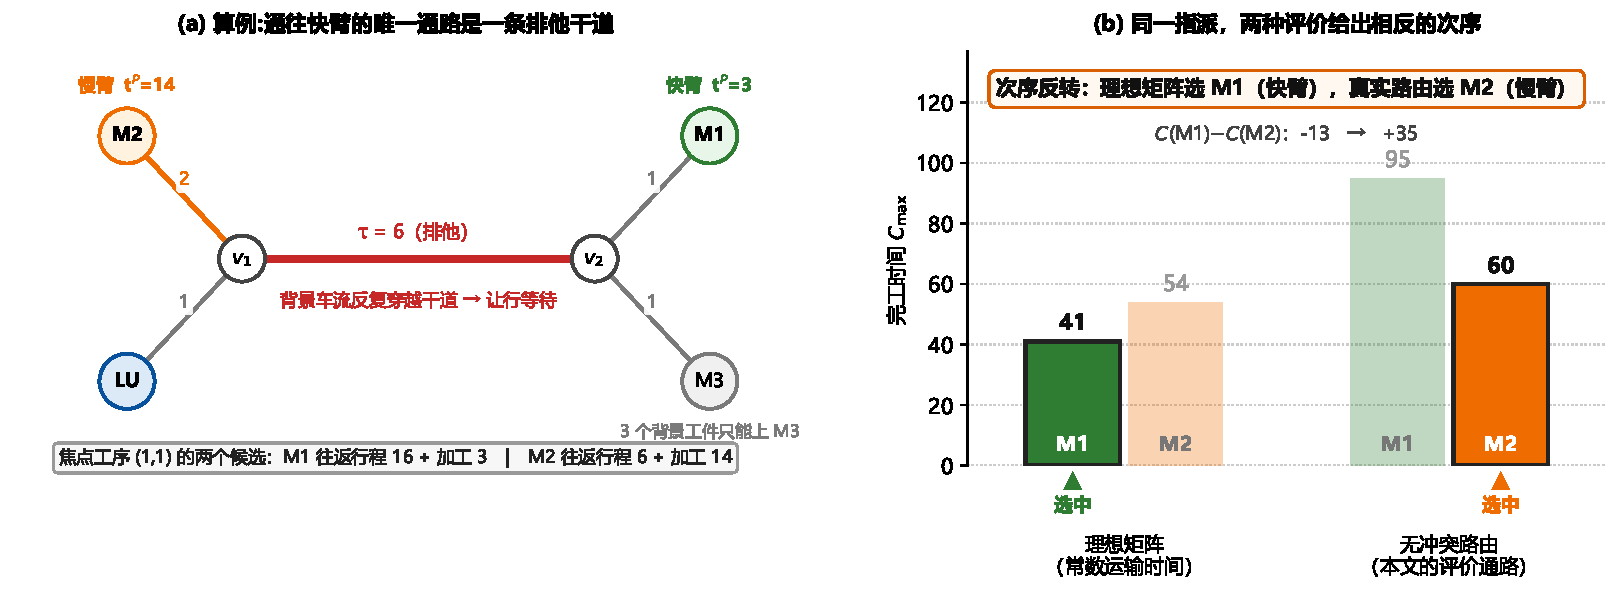
\includegraphics[width=\textwidth]{fig/fig_motivating.pdf}
\Description{Two panels. The left panel is a small shop network in which the only
route to a fast arm passes through an exclusive trunk corridor, while a slow arm
hangs on its own branch. The right panel shows makespan for the same two machine
assignments evaluated twice: under a constant travel-time matrix the fast arm
wins, under conflict-free routing the slow arm wins, so the ranking reverses.}
\caption{动机算例:同一个指派决策,两种评价方式给出相反的次序。(a) 通往快臂 M1 的唯一通路是
一条排他干道($\tau=6$),慢臂 M2 挂在自有支路上;三个背景工件只能上 M3,因而反复穿越干道。
(b) 焦点工序的两个候选各评价两次。常数运输时间矩阵看不见让行等待,故按"较短加工 $+$ 较长行驶"
选中快臂;把同样这两个指派交给无冲突路由重新评价,慢臂反而更优。差值由 $-13$ 翻为 $+35$。
本图是一个\emph{存在性演示}而非统计结论——它要说明反转会发生,不是反转普遍发生;在围绕该
算例的 $1200$ 组参数网格中有 $205$ 组($17\%$)出现反转,故它也不是参数空间里的孤点。}
\label{fig:motivating}
%% 由 fig/fig_motivating.py 从 clbs/output/motivating.json 生成,后者由
%% clbs/tools/motivating.py --sweep 用与论文同一套解码器算出((b) 的四个数不是示意值:
%% 理想矩阵 = decode(conflict_free=False),无冲突路由 = decode(conflict_free=True))。
%% 算例:4 工件 / 3 机械臂 / 6 节点 / 5 走廊 / 2 AGV,delta_return=1,规则派车。
%% 注意:不要复用 fig/fig_intro_problem_new.pdf,那张图画的是上一篇论文
%% "邻近性对可用性"的场景,不是走廊争用。
\end{figure*}

\subsection{与最接近工作的差距}

现有工作或者每次只处理这一耦合的一侧,或者只在单一方向上把两侧连接起来。无冲突多机器人
路由高度重视争用——终身式(lifelong)问题的表述甚至通过重塑边权把交通从瓶颈处引
开~\cite{zhang2024guidance}——但任务及其释放时刻与端点均来自规划器之外,规划器因而无权
质疑产生这些任务的指派。拥堵感知的车队控制同样对拥堵路段施加惩罚,却是在一组固定的运输
订单上做派车,且以局部车辆密度作为拥堵的代理度量~\cite{kim2026congestion}。

在调度一侧,这一组合已被形式化:带无冲突运输约束的柔性作业车间调度问题把"具有位置相关
加工时间的可选机器工序"与"无冲突车辆路由"耦合起来,并由基于逻辑的 Benders 分解将其基准
算例求解至可证最优~\cite{vanos2026exact}。本文采用该问题类,而非声称提出它。仍然敞开的
是启发式区间——算例一旦超出精确分解可及的规模便进入该区间,而在那里耦合仍是单向的。
两阶段方案先固定排程、再针对它消解车辆冲突~\cite{sun2023integrated},因此第二阶段发现的
争用无法回过头修改第一阶段。与本文最接近的工作加入了一个反馈步骤,但正如其局限性小节
自述,它"主要作为两阶段顺序优化策略而非完全动态的实时闭环系统运作",依赖的是"一次性的
反馈调整"~\cite{li2026framework}。该设计带来两个后果,且都是结构性的而非偶然的:反馈只
调整时间轴而不修改任何指派;并且它只施加于单个当前最优解一次,而不施加于搜索所考察的
每一个候选解。此外,该工作是在每道工序仅一台可选机器、加工时间固定的作业车间基准上
展开的,上文那种改派权衡在其中根本无从出现。

概括起来,两类最接近的工作各缺一半:一类具备机器柔性却在常数运输时间矩阵上排产,看不见
拥堵;另一类具备真正的无冲突路由却没有柔性,指派由算例固定。本文开头那句"最短走廊拥堵
时,去一台更慢但连通性更好的机械臂可能更优",在它们的模型里连表述都无法完成。

\subsection{本文方法}

本文在两种意义上闭合这个回路,并逐项量化每一种意义值多少。框架保留双层结构——上层决定
机器指派与工序排序,下层以时间窗预约生成无冲突路径——但沿两条通路连接两层。

\emph{评价通路}把每一代中每一个候选解的适应度,定义为下层真正为其规划过路径之后得到的
完工时间。于是让行延误进入搜索所优化的目标本身,而不再是事后的可行性校验。这一步的想法
并不深刻,深刻之处在于它很贵:一次完整的无冲突解码比在理想最短路矩阵上解码昂贵一个数量级
以上,因此在固定算力下它必须与它所挤占的那些额外评价次数竞争。据我们所知,此前没有工作
量化过这笔交换是否划算;\cite{li2026framework} 的作者本人正是把"将该机制扩展为完全迭代
的回路"列为未来工作。

\emph{决策通路}上承重的机制是\emph{预约表感知的车辆派遣}。选车不再依据理想最短路对到达
时刻的估计,而是对预约表做一次两段式试探:对每一个候选车辆,依次询问"取货段"与"送货段"
在当前预约状态下实际可行的最早完成时刻,再取其中最优者。它所替换的恰是文
献~\cite{li2026framework} 正在使用的空闲优先规则,因此这一机制针对的是现行的发表实践,
而不是一个假想的弱基线。为使它在同挂钟预算下付得起,本文给出两项可证保持最优选择的降本:
基于可采纳下界的剪枝,以及胜者路径的复用。

我们同样实现并考察了更具雄心的第三条接口:让下层不只返回时间,而返回对关键链的归因——
把关键链从工序序列扩展为工序与运输交替的链,并给每一环标注五类成因之一
(\texttt{工序}、\texttt{机器}、\texttt{上游}、\texttt{车辆}、\texttt{走廊}),其中最后一类
指明被争用的路段及让行发生的时段;再由两族算子据此行动:\emph{改派}把工序移到经由争用
较轻的网络区域可达的机械臂(改变地点),\emph{错峰}把被阻塞的工序提前或把阻塞者推后
(改变时间)。这一设计在直觉上比预约表试探更有吸引力,但在同挂钟预算下其增益未获证实。
本文如实报告这一点,并把它与走廊时段定价一并作为受控负对照(第~\ref{sec:Chapter_V}~节),
用以说明为何在若干候选接口中最终选定了预约表感知派遣这一个。这些负对照不是本文的结论,
而是本文设计取舍的正当理由。

\subsection{主要结果}

为使"闭环"与"具体机制"两笔账互不冒领,我们构造了一个四级基线阶梯,其中前两级分别复现两篇
已发表工作的结构:\textbf{B0} 为开环规划加真实执行,对应~\cite{li2026framework};\textbf{B0+}
在冻结排产上只把车辆指派换成感知冲突的,对应~\cite{sun2023integrated} 的两阶段结构;
\textbf{B1} 为闭环规划加规则派车;\textbf{B2} 为本文方法。这四级构成"是否闭环"与"派车方式"
的 $2\times2$ 析因,故每次只动一个因子的对比才可用于归因。所有方案——无论其计划从何而来——
都必须放进同一个无冲突路由器执行并通过同一个独立校验器,报告的都是可实现的完工时间。

结果显示两条主张各自成立。把拥堵搬进搜索目标(固定派车方式)使完工时间降低
\GainLoopRule{}($p=\PLoopRule$),这是闭环本身的价值;在闭环内部把规则派车替换为预约表
感知派遣(信息完全对等,只差派车一处决策)再降低 \GainProbeLoop{}($p=\PProbeLoop$),
这是该具体机制的价值;端到端相对文献结构降低 \GainEndToEnd{},\WinEndToEnd{} 胜
\LoseEndToEnd{} 负($p=\PEndToEnd$)。两项降本使派遣机制的加速比达到 \SpeedupProbe{} 倍、
路由调用减少 \RouteCallCut{},单次评价的成本倍数从 \CostMultBefore{} 压到
\CostMultAfter{},这正是它在同挂钟预算下能够转为净收益的原因。

两条机制都显著,但\emph{不可互相替代}。开环下的试探派车值 \GainProbeOpen{}
($p=\PProbeOpen$),远小于闭环的 \GainLoopRule{};端到端 \GainEndToEnd{} 接近两者独立时
应有的 \GainIndepProduct{},呈近加性而非正交互。这也是我们坚持报告 $2\times2$ 析因而非
一条消融链的原因:只有分因子才能看见"主效应大、次效应小但仍显著"。

稳健性方面,上述增益在 \NCases{} 个受控算例格上取得,这些算例格沿三个因子族逐一单变——布局
(争用强度覆盖 \ContentionLo{} 至 \ContentionHi{})、车臂比与柔性。
第~\ref{sec:whichcongestion}~小节给出逐族结果,而两个效应在这一层的表现截然不同,这个差别
本身就是一条结论。闭环增益在
\CellsSigLoop{}/\NCases{} 个格上自身即达显著,并随争用强度大体上升,可以按族解读;闭环内的
试探增益则只有 \CellsSigProbe{}/\NCases{} 个格达显著,车臂比族的四个水平上符号交替且无一格
能与零区分。因此我们只主张该机制在合计口径上为正,\emph{不}主张它有一个可指认的适用区间——
以 \NSeeds{} 个种子的逐格分辨率,那样的主张会是在读噪声。

\subsection{实验协议}

上述任何一条结论的成立都要求比通常做法更严格的实验协议,原因是我们亲历过的三个陷阱。
第一,各机制的单次评价成本相差极大,最贵与最便宜之间可达两个数量级,因此在\emph{相同代数}
下比较等于把一个机制多消耗的算力也记作它的功劳;改用同挂钟预算后,若干表面上的增益会
反转。第二,在拥堵算例上完工时间的种子间离散度超过不同方案之间的差距,单个种子几乎可以
把各方案排成任意次序,故所有比较均在多个随机种子上以配对 Wilcoxon 检验进行。第三个陷阱
更隐蔽,并且曾使我们得出过错误结论:消融必须每次只改变一个因子,而"每一行在上一行基础上
增加一个机制"的链式消融只有在各行确实只差一个因子时才满足这一点。我们的早期设计并不满足,
而被混淆的那个对比会把一个机制报告为显著有益,去混淆后的对比却报告它显著有害——同一批
运行,相反的符号,两者都显著。

算例本身也是一个要设计的对象。集中在上下料出口处的拥堵会被所有工件在所有指派下穿越,
它只是抬高每一张排程的延误,却不给任何机制可利用的余地。因此我们生成的算例以网络容量
而非距离作为旋钮来调节争用强度,并用一对仅在站口断面宽度上有差别的匹配算例,把"调度器
可以绕开的拥堵"与"绕不开的拥堵"区分开来。

本文的贡献如下。

\begin{enumerate}[leftmargin=*]

\item \textbf{问题层:一个在最接近的两类工作中都无法表述的权衡。} 机器柔性、加工效率异构
与走廊拥堵三者同时在场,且拥堵进入目标函数。由此"最短走廊拥堵时,去一台更慢但连通性更好
的机械臂可能更优"成为一个真实的决策;而在具备柔性但用常数运输时间矩阵排产的模型
里~\cite{sun2023integrated},以及在具备真正无冲突路由但机器由算例固定的模型
里~\cite{li2026framework},这句话都无法被表述。我们在既有的带无冲突运输约束的柔性作业
车间调度问题类~\cite{vanos2026exact} 内工作,采用该问题类而不声称提出它,并补充一个可控
的争用强度刻画,使"何时值得管拥堵"成为可回答的问题。

\item \textbf{框架层:闭环的价值被首次量化。} 把无冲突路由放进适应度函数这一想法本身并不
深刻,深刻之处在于它很贵,因而从未有人量过它值多少——\cite{li2026framework} 的作者本人正
把完全迭代的回路列为未来工作。本文在同挂钟预算下给出这笔交换的汇率:相对该文献的忠实
结构,闭环使完工时间降低 \GainLoopRule{}($p=\PLoopRule$),在预约表感知派遣下达到
\GainLoopProbe{}($p=\PLoopProbe$)。贡献是"定量"加"让它付得起",而不是这个念头本身。

\item \textbf{机制层:预约表探测式派车,以及让它付得起的降本。} 在闭环内部,该机制值
\GainProbeLoop{}($p=\PProbeLoop$);它替换的正是文献~\cite{li2026framework} 在用的空闲
优先规则,因此打的是现行的发表实践。两项可证保持最优选择的优化——基于可采纳下界的剪枝与
胜者路径复用——带来 \SpeedupProbe{} 倍加速、路由调用减少 \RouteCallCut{},把单次评价的
成本倍数从 \CostMultBefore{} 压到 \CostMultAfter{}。机制层面的解释是:AGV 之间是同构的,
车与车唯一的差别在于站位与路是否通得过,因此选车是一个纯粹的拥堵决策,信息能够全额兑现;
而选臂还掺入加工时长,后者往往压过走廊差异。

\item \textbf{角色分工,以及一条关于分辨率的负结论。} 闭环是主效应,在
\CellsSigLoop{}/\NCases{} 个算例格上自身即达显著;预约表感知派遣是量级小得多的次效应,
在开环与闭环下的合计口径上都显著,端到端接近独立乘积(近加性),而开环试探单独远不能代替
闭环。但它逐格只有 \CellsSigProbe{}/\NCases{} 格显著,车臂比族的四个水平上符号交替且无一
显著,故我们\emph{不}报告它的适用区间。这一条把"机制有效"与"知道它在哪里有效"分开:后者
需要的种子数远多于前者,而这一点在同类工作中很少被区分。

\item \textbf{方法层:一套把机制与算力分开的实验装置。} 包括争用强度可控的算例生成
(争用强度覆盖 \ContentionLo{} 至 \ContentionHi{})、统一执行器(任何来源的计划都经同一个
仿真器与同一个独立校验器)、同挂钟而非同代数的预算口径,以及四级基线阶梯且每一级对应一篇
真实发表的结构。我们并附两个受控负对照:走廊时段定价在同等算力下系统性有害,冲突凭证制导
的局部搜索(改派与错峰两族算子)命中率过低、不足以抵偿它消耗的解码次数。这些负对照不是
本文的结论,而是"我们为何选定这个设计"的正当理由。

\end{enumerate}

\subsection{论文组织}

本文余下部分组织如下。第~\ref{sec:Chapter_II}~节回顾相关工作,包括考虑运输的柔性作业车间
调度、任务外生的无冲突路由,以及两者的一体化表述,并定位本文的缺口。
第~\ref{sec:Chapter_III}~节给出问题描述与数学模型,含符号表与编号的建模假设。
第~\ref{sec:Chapter_IV}~节详述闭环双层框架:两条反馈通路、下层的时间窗预约路由、上层的
编码与事件驱动解码、预约表感知的车辆派遣及其两项降本,并给出复杂度与代价分析。
第~\ref{sec:Chapter_V}~节报告实验协议与结果:四级基线阶梯、主结果、主效应与不可替代性、
逐因子族的稳健性、消融与受控负对照,以及案例的关键链归因。第~\ref{sec:Chapter_VI}~节总结
全文并讨论局限与后续方向。

全文符号汇总于表~\ref{tab:notation}。



\section{相关工作}
\label{sec:Chapter_II}

本文的问题位于两支长期各自独立发展的文献之间:考虑运输的柔性作业车间调度,它决定什么在
何处以何种次序被加工,却把车辆抽象掉;以及无冲突多机器人路由,它在时空上消解车辆争用,
但任务来自别处。下面依次回顾两者,再回顾数量较少的一体化工作,并在最后定位本文的缺口。

\subsection{考虑运输的柔性作业车间调度}

含加工机器与运输车辆的柔性作业车间调度问题(FJSP\_PT)通过把物料移动纳入排程来扩展 FJSP。
Xin 等~\cite{xin2025review} 系统综述了该领域至 2023 年的进展,梳理其假设、约束、目标与
基准算例,并把求解方法分为精确、启发式、元启发式与群智能几类。其中占主导地位的建模约定
是一个按位置对索引的常数行驶时间矩阵:车辆把工件从 $a$ 移到 $b$ 需要固定的 $t(a,b)$,
与车间里同时发生的其他事情无关。于是车辆只是一种\emph{能力}资源——它们为工件而竞争,
却从不为空间而竞争。

这一传统在组合优化一侧进展迅速。Meng 等~\cite{meng2025cp} 给出多 AGV 情形下 FJSP 的约束
规划模型,关闭了 29 个此前开放的基准算例并改进了 27 个最优已知解,并与一个由约束规划辅助
的双种群遗传算法相配合。Qin 等~\cite{qin2026knowledge} 把质量--多样性存档与 Q 学习的区域
选择结合,并设计了由 AGV 与关键路径共同制导的局部搜索。Fu 等~\cite{fu2025integrated} 用
改进遗传算法在柔性装配车间中一体化地决策生产与物流。但在上述全部工作中,运输时长都是从
矩阵中读出的,因此一辆车永远不会被另一辆车延误。

综述本身明确指出这是一个局限而非已成定论的建模选择,它观察到"目前多数调度问题的假设过多",
而这些假设"会降低问题复杂度,甚至改变问题的性质,例如当运输车辆数量足够多
时"~\cite{xin2025review};并进一步指出,工件到达机器的时刻在实践中受交通拥堵影响,而
加工--运输两阶段流动中隐含的依赖关系必须先被处理,一张排程才谈得上可行,更不必说
鲁棒。

\subsection{任务外生的无冲突路由与拥堵感知派车}

互补的另一支文献把争用本身当作研究对象。在多智能体路径规划、特别是其终身式变体中,多个
智能体必须在共享图上无碰撞地行进,而拥堵被公认会在远未达到容量上限时就已损害吞吐。
Zhang 等~\cite{zhang2024guidance} 的做法是优化一张制导图,用其边权把智能体从瓶颈处引开
并抑制迎面运动,从而提升若干终身式求解器的吞吐。在制造场景中,Kim 与
Kim~\cite{kim2026congestion} 为大规模 AGV 车队提出拥堵函数、拥堵惩罚与拥堵感知的派车
规则,并在离散事件仿真中加以评估。

这支文献有两个特征对本文尤为重要。第一,任务是外生的:其释放时刻、起点与终点都是交给
路由器的输入,路由器因而从来没有资格质疑产生这些任务的那个指派。第二,凡对拥堵作量化之处,
所用的通常是一个代理量——\cite{kim2026congestion} 中的局部车辆密度、\cite{zhang2024guidance}
中离线学到的边权——而不是某一次具体的预约实际给某一个具体任务造成的延误。这一区别决定了
反馈能携带什么:代理量只能说明"此处大体拥挤",而具体的让行事件才能指名"哪一段、哪个时段、
被谁先占",后者才是上层据以决定"是把工序换个地方,还是仅仅换个时间"所需的信息。

\subsection{调度与无冲突路由的一体化:反馈深度与本文定位}

把两者耦合起来的工作数量较少。在精确求解一侧,van Os 与 Basten~\cite{vanos2026exact}
形式化了带无冲突运输约束的柔性作业车间调度问题,它把"具有位置相关加工时间的可选机器工序"
与"无冲突车辆路由"结合起来,并以基于逻辑的 Benders 分解求解:约束规划主问题给出排程,
整数规划子问题为车辆规划路径并返回由冲突驱动的割。多数基准算例被求解至可证最优,其中约
一半相对此前的启发式方法把完工时间改进了至少 10\%。该方法受限于精确分解可及的算例规模,
其作者亦指出,更积极地利用"关于不可行性成因的信息"是自然的下一步。本文采用这一问题类,
并把上述"由不可行成因反馈到可行动决策"的思路移到启发式区间;第~\ref{sec:Chapter_IV}~节的
预约表试探正可视为该思路在启发式框架中的对应物。

在启发式一侧,耦合仍是单向的。Sun 等~\cite{sun2023integrated} 先用混合遗传算法排产,再在
第二阶段用 AGV 编码的遗传算法与时间窗 Dijkstra 消解 AGV 冲突;第二阶段发现的争用无法回过
头修改第一阶段。Li 等~\cite{li2026framework} 最接近一个回路:其调度层用强化学习,任务分配
由甘特图导出,再由基于优先级搜索的路径层把实现的运输时长反馈回时间轴。该文自己的局限性
小节把结果描述为"主要作为两阶段顺序优化策略而非完全动态的实时闭环系统"运作,依赖"一次性
的反馈调整",并指出"最终解的全局最优性部分依赖于初始排程的质量"。其反馈只携带时间,因而
只能沿时间轴平移排程而无法修改任何指派;并且其基准是每道工序仅一台可选机器的经典作业车间
算例,改派在其中根本不是一个决策。

本文的缺口正落在"闭环深度"上,而不落在"是否考虑冲突"上。上述两项工作都已认真对待冲突;
区别在于路由结果到达调度决策的\emph{频次}与\emph{内容}:是每一代对每一个候选解都到达,
还是只对单个当前最优解到达一次;是只携带时间,还是携带足以支持改派的信息。

关键链推理在作业车间局部搜索中早已成熟,近期的 FJSP\_PT 工作也在考虑运输的前提下加以
运用~\cite{qin2026knowledge}。当路由变为无冲突之后发生变化的是诊断的\emph{内容}。基于
行驶时间矩阵算出的关键链,可以把一次迟到的开工归因于缓慢的前驱或繁忙的机器,却无法把它
归因于某条走廊,因为在那个模型里走廊并不作为被争用的资源而存在。一旦占用被按时间窗预约,
一次迟到的开工便可被追溯到具体的路段、具体的时段,以及先行预约它的那个任务。

对算例设计,\cite{xin2025review} 亦指出该领域的算例"主要在规模上有差别,缺少针对关键问题
参数取值的专门设计",并特别把平均运输时间与平均加工时间之比 $\bar{T}_t/\bar{T}_p$ 列为
极可能影响算法表现的量,呼吁扩充测试集。本文在此之上补充一个只有在路由被显式建模后才可见
的参数:一个算例的拥堵中有多少是与指派相关的。集中在上下料出口的拥堵会被所有工件在所有
指派下穿越,因而不奖励任何决策;而只服务于部分机器的走廊上的拥堵则可以被绕开。两个
$\bar{T}_t/\bar{T}_p$ 完全相同的算例,留给调度机制的可操作余地可能完全不同。本文据此生成
争用强度可控的算例(第~\ref{sec:Chapter_V}~节),并对实验协议提出一项要求:当各机制的单次
评价成本相差达两个数量级时,在相同迭代次数下比较所测得的并非其所声称的东西,且误差方向
并不随机——它偏向每次迭代做更多工作的那一个,而那通常正是被提出的方法。

表~\ref{tab:related} 汇总了上述比较。本文工作的问题类并不新,它就是~\cite{vanos2026exact}
所形式化的那一个,本文采用它;敞开的是启发式区间——算例在此超出精确分解可及的规模,而调度
与路由之间的耦合在此仍然或缺失、或单向、或只对单个当前最优解施加一次。本文的贡献是在这个
区间内给出一个闭合到每一个候选解的双层框架,指认其中真正承重的那一个层间机制(预约表感知
的车辆派遣),用可证等价的降本使它在同等算力下付得起,并量化它相对闭环主效应的角色与量级。

\begin{table}[t]
\caption{与最接近的几支工作的定位对比。"机器异构"指一道工序有多台可选机器且加工时间随
机器而变;"耦合频次"指路由结果以何种频次、沿何种方向到达调度决策;最后一列是穿过层间
接口的内容。本文实现了实现时间、冲突凭证与走廊价格三类接口,并按各自的代价与收益逐一
报告,其中承重的是预约表试探。}
\label{tab:related}
\footnotesize
\begin{tabular}{@{}lclll l@{}}
\toprule
工作类别 & 文献 & 机器异构 & 车辆争用 & 耦合频次 & 反馈内容 \\
\midrule
FJSP\_PT 元启发式 & \cite{meng2025cp,qin2026knowledge,fu2025integrated}
  & 有 & 常数矩阵 & --- & --- \\
终身式 MAPF & \cite{zhang2024guidance}
  & --- & 无冲突 & 任务外生 & 边权 \\
拥堵感知派车 & \cite{kim2026congestion}
  & 无 & 密度代理量 & 单向 & 拥堵惩罚 \\
两阶段 FJSP + 路由 & \cite{sun2023integrated}
  & 有 & 无冲突 & 单向 & 无 \\
强化学习调度 + PBS & \cite{li2026framework}
  & 无 & 无冲突 & 一次性修正 & 到达时刻 \\
精确 LBBD & \cite{vanos2026exact}
  & 有 & 无冲突 & 主--子问题 & 冲突驱动割 \\
\textbf{本文} &
  & 有 & 无冲突 & 每个候选解 & 实现时间 + 预约表试探 \\
\bottomrule
\end{tabular}
\end{table}


\section{问题描述与数学模型}
\label{sec:Chapter_III}
\subsection{问题描述}

一个算例由 $n$ 个工件、$N_M$ 台机械臂与 $N_A$ 辆自动导引车构成,它们在一个以图表示的车间
中运行。工件 $j$ 具有固定的 $n_j$ 道工序链 $O_{j1}\to\cdots\to O_{jn_j}$;工序 $O_{ji}$
可在其可选集 $\Omega_{ji}\subseteq M$ 中的任一机械臂上加工,在机械臂 $m$ 上耗时
$t^P_{jim}$,该值取决于所选的机械臂。机械臂占据图中的固定节点,工件由车队在这些节点之间
搬运。求解一个算例意味着同时确定四组决策:

\begin{enumerate}[label=(\roman*),leftmargin=*,topsep=2pt,itemsep=1pt]
\item 把每道工序 $O_{ji}$ 指派给某台机械臂 $m\in\Omega_{ji}$;
\item 为每台机械臂上被指派的工序排序;
\item 把由此派生的运输任务指派给车辆,并为每辆车的任务排序;
\item 为每一次车辆移动在图上规划路径,要求在时间与空间上无冲突,允许等待。
\end{enumerate}

目标是最小化完工时间 $C_{\max}$。

\begin{table}[t]
\caption{符号说明。}
\label{tab:notation}
\small
\begin{tabular}{@{}ll@{}}
\toprule
符号 & 含义 \\
\midrule
$J=\{1,\dots,n\}$, $O_{ji}$ & 工件集合;工件 $j$ 的第 $i$ 道工序,$i\le n_j$ \\
$M=\{1,\dots,N_M\}$, $\Omega_{ji}\subseteq M$ & 机械臂集合;$O_{ji}$ 的可选机械臂集 \\
$t^P_{jim}$ & $O_{ji}$ 在机械臂 $m\in\Omega_{ji}$ 上的加工时间 \\
$K=\{1,\dots,N_A\}$ & 同构的单载量车辆 \\
$G=(V,E)$, $\tau_e$ & 车间图;走廊 $e\in E$ 的通行时间 \\
$v_0$, $\mathrm{loc}(m)$ & 上下料站;机械臂 $m$ 所在节点 \\
$t^{*}(a,b)$ & $G$ 中 $a$ 到 $b$ 的最短路时间,不计争用 \\
$\delta_{\mathrm{ret}}\in\{0,1\}$ & 完工工件是否返回 $v_0$(基准取 $1$) \\
$S_{ji}$, $C_{ji}$, $A_{ji}$ & $O_{ji}$ 的开工、完工与物料到达时刻 \\
$C_{\max}$ & 完工时间 \\
\bottomrule
\end{tabular}
\end{table}

\subsection{建模假设}
\label{sec:assumptions}

\begin{enumerate}[label=\textbf{A\arabic*.},leftmargin=*,topsep=2pt,itemsep=2pt]
\item \textbf{静态算例与完全信息。} 全部 $n$ 个工件在 $t=0$ 时刻均已位于 $v_0$,不设释放
时刻与交货期。加工数据、布局 $G$ 与车辆状态在规划时均为已知。

\item \textbf{工件。} 每个工件具有固定的前后约束链。加工与运输均不可抢占,工件不可拆分,
不同工件之间不存在外生的先后约束。

\item \textbf{机械臂:部分柔性且工时异构。} 每道工序 $O_{ji}$ 可在任一
$m\in\Omega_{ji}$ 上加工,多数工序满足 $|\Omega_{ji}|\ge 2$,完全柔性
$\Omega_{ji}=M$ 是其特例。加工时间在\emph{无关机器}(unrelated)意义上与机器有关:当
$m\neq m'$ 时,$t^P_{jim}$ 与 $t^P_{jim'}$ 之间不必存在任何关系。一台机械臂同时只加工
一道工序,在计划期内不发生故障,与顺序相关的准备时间被并入 $t^P_{jim}$。

\item \textbf{缓冲区与装卸。} 每台机械臂的输入、输出缓冲区以及 $v_0$ 处的存储容量充裕,
因而不发生阻塞。装载与卸载时间可忽略,且不占用机械臂。

\item \textbf{车辆。} $N_A$ 辆车同构、单载量,空载与满载均以恒定速度行驶,不建模加减速与
电量。一个运输任务是一次单程移动——从 $v_0$ 到第一台机械臂、在前后两台不同机械臂之间,
或当 $\delta_{\mathrm{ret}}=1$ 时从最后一台机械臂返回 $v_0$;任一车辆可执行任一任务,
因此同一工件的连续移动可以在不同车辆之间接力。卸载之后车辆不被强制返回 $v_0$,而是按其
自身的任务链重新占位,且其出发时刻可由路由层推迟。

\item \textbf{路网与无冲突性。} $G$ 强连通,各走廊的通行时间 $\tau_e$ 为已知常数。走廊是
\emph{排他}资源:$e$ 的两个方向共享同一份预约,因而任一时刻最多一辆车占用 $e$,这同时
排除了迎面冲突与同向超车。占用区间取半开形式 $[t,\,t+\tau_e)$,故第二辆车可以恰好在
$t+\tau_e$ 进入。节点上设有容量充裕的停靠位,它与通行资源相互独立;因此等待发生在停靠位
上,并且总是被允许的。

\item \textbf{构造性的无死锁。} 路径以走廊资源上的时间窗预约方式规划,新路径只能占用空闲
的时间窗。结合 A4 与 A6,这使得任何指派、排序与任务链都可被解码为一张无冲突、无死锁且
完工时间有限的排程,因而永远不需要对不可行解做修复。

\item \textbf{不在建模范围内。} 机器与车辆故障、有限缓冲与阻塞、电池充电,以及工件的动态
到达,均留待后续工作。
\end{enumerate}

其中 A1、A2、A4 与 A5 在 FJSP\_PT 文献中是标准假设~\cite{xin2025review}。真正塑造本文的
是 A3(部分柔性机械臂上与机器相关的加工时间)与 A6(把争用表述为显式的排他资源约束,而不是
一个常数行驶时间矩阵),以及由此导出的一个事实:运输时长是路由决策的输出,而不是输入参数。

\subsection{决策变量与派生的运输任务}

令 $x_{jim}\in\{0,1\}$ 表示 $O_{ji}$ 被指派给机械臂 $m$,记 $\mathrm{m}(j,i)$ 为如此选定
的机械臂,$d_{ji}=\mathrm{loc}(\mathrm{m}(j,i))$ 为其所在节点。当 $\delta_{\mathrm{ret}}=1$
时,为每个工件追加一道位于 $v_0$、加工时间为零的\emph{伪工序} $O_{j,n_j+1}$,用以表示完工
工件的返回;这样可使完工时间的定义保持统一。

与车辆路径问题不同,运输任务并不是输入的一部分,而是由指派\emph{派生}出来的:
\begin{equation}
\label{eq:tasks}
\mathcal{T}(x)=\Bigl\{\,(j,i)\ :\ d_{j,i-1}\neq d_{ji}\,\Bigr\},
\qquad d_{j0}\equiv v_0 ,
\end{equation}
其中任务 $(j,i)$ 把工件 $j$ 从 $d_{j,i-1}$ 搬到 $d_{ji}$,并在
$r_{ji}=C_{j,i-1}$ 时刻就绪(约定 $C_{j0}=0$)。若前后两道工序被放在同一台机械臂上,则不
产生任何任务。因此,运输任务的\emph{数量}与\emph{端点}都是决策组 (i) 的后果:一个把工件
始终留在同一台机械臂上的指派只需搬运两次,而一个每道工序都换臂的指派则需搬运 $n_j+1$ 次。
任务到车辆的指派用 $y_{tk}\in\{0,1\}$ 表示,对每个 $t\in\mathcal{T}(x)$ 有
$\sum_{k\in K}y_{tk}=1$,且分配给同一辆车的任务是全序的。

这一点值得强调:在常数行驶时间矩阵的模型中,运输量是给定的;而在本文的模型中,上层的指派
决策同时决定了要搬多少次、从哪搬到哪,以及这些搬运会在哪些走廊上彼此争用。

\subsection{时序关系与可行性条件}

记 $p_{ji}=\sum_{m\in\Omega_{ji}}x_{jim}t^P_{jim}$ 为实现的加工时间。指派、前后约束与
机械臂的单件加工能力给出
\begin{align}
\sum_{m\in\Omega_{ji}} x_{jim} &= 1, & \forall j,i,
\label{eq:assign}\\
C_{ji} &= S_{ji}+p_{ji}, & \forall j,i,
\label{eq:dur}\\
S_{ji} &\ \ge\ A_{ji}, & \forall j,i,
\label{eq:material}\\
S_{j'i'}\ \ge\ C_{ji}\ \ \vee\ \ S_{ji} &\ \ge\ C_{j'i'}
& \forall (j,i)\neq(j',i')\ \text{位于同一机械臂},
\label{eq:disj}
\end{align}
其中 $A_{ji}$ 是工件实际出现在 $d_{ji}$ 的时刻。若 $(j,i)\notin\mathcal{T}(x)$,则工件
本已在该处,$A_{ji}=C_{j,i-1}$。否则 $A_{ji}$ 由承运任务 $(j,i)$ 的那辆车产生:记
$a^{\mathrm{E}}_{ji}$ 为该车经空载段到达取货节点的时刻,则
\begin{equation}
\label{eq:load}
\ell_{ji}=\max\bigl(a^{\mathrm{E}}_{ji},\ r_{ji}\bigr),
\qquad
A_{ji}=\text{于 } \ell_{ji} \text{ 出发的满载段的到达时刻},
\end{equation}
即车辆可以等工件,工件也可以等车辆。无论空载段还是满载段,每一段都是 $G$ 中的一条通路
$(e_1,\dots,e_q)$,其走廊进入时刻 $\theta_1,\dots,\theta_q$ 满足
\begin{equation}
\label{eq:walk}
\theta_1 \ \ge\ \sigma, \qquad
\theta_{l+1}\ \ge\ \theta_l+\tau_{e_l}, \quad l=1,\dots,q-1,
\end{equation}
其中 $\sigma$ 是该段可以开始的时刻;上述不等式取严格不等号的时刻恰好就是车辆在停靠位等待
的时刻,而该段在 $\theta_q+\tau_{e_q}$ 结束。最后是争用约束:
\begin{equation}
\label{eq:excl}
\bigl[\theta,\ \theta+\tau_e\bigr)\ \cap\
\bigl[\theta',\ \theta'+\tau_e\bigr)\ =\ \emptyset
\end{equation}
该式对同一走廊 $e$ 的任意两次不同占用都成立,与方向无关,也与涉及哪些车辆无关。目标函数为
\begin{equation}
\label{eq:obj}
\min\ C_{\max},\qquad
C_{\max}=\max_{j\in J}\ C_{j,\,n_j+\delta_{\mathrm{ret}}} .
\end{equation}

有两个推论值得记录,因为第~\ref{sec:Chapter_IV}~节的算法正建立在它们之上。第一,在任何
半活动排程中,\eqref{eq:material} 与 \eqref{eq:disj} 可收紧为
\begin{equation}
\label{eq:bind}
S_{ji}=\max\bigl(A_{ji},\ F_{\mathrm{m}(j,i)}\bigr),
\end{equation}
其中 $F_m$ 是机械臂 $m$ 上排在 $O_{ji}$ 之前那道工序的完工时刻。于是开工时刻恰由两种成因
之一支配,且两者中哪一个取到最大值是良定义的;正是这一点使得后文把一次延误归因于某个成因
成为有意义的判定,而不是启发式的猜测。第二,\eqref{eq:excl} 是模型中唯一通过\emph{空间}
而非通过共享机器来耦合不同工件的约束。

\subsection{与 FJSP\_PT 的关系}

删去~\eqref{eq:excl} 后各段彼此独立,于是每一段都可以走最短路,且 \eqref{eq:walk} 处处
取等号。运输时长随之退化为常数矩阵 $t^{*}(a,b)$,模型也就变成标准的考虑运输的柔性作业车间
调度问题。因此两个问题之间的全部差别只是一族约束——以及随之而来的一个事实:一次移动的时长
不再是参数,而是由所有车辆的路径共同决定的变量。同一松弛还提供了自然的乐观估计 $t^{*}$,
它在后文既用作下界,也在开环基线中充当派车器对到达时刻的估计。

\subsection{计算复杂度}

\begin{prop}
\label{prop:np_hard}
由 \eqref{eq:assign}--\eqref{eq:obj} 定义的问题是强 NP 难的;且当所有工序均满足
$\Omega_{ji}=M$ 时依然如此。
\end{prop}

\begin{proof}
限制到如下算例:对所有 $e\in E$ 有 $\tau_e=0$,每台机械臂各由一条专用走廊与 $v_0$ 相连,
且 $N_A=n$。此时每一段行驶耗时为零、占用的半开区间 $[t,t)=\emptyset$,故 \eqref{eq:excl}
恒真,任何车辆都无法延误另一辆车;又因每个工件独占一辆车,\eqref{eq:load} 从不起作用,
$A_{ji}=C_{j,i-1}$。余下的正是取 $A_{ji}=C_{j,i-1}$ 的
\eqref{eq:assign}--\eqref{eq:disj},也就是无关机器情形下的柔性作业车间调度问题。它的两个
特例已是强 NP 难的:处处取 $|\Omega_{ji}|=1$ 时退化为经典作业车间问题,在三台机器下即为
强 NP 难~\cite{garey1976complexity};取 $\Omega_{ji}=M$ 且 $n_j=1$ 时退化为无关并行机上
的完工时间最小化问题,它包含同型并行机调度,在机器数可变时为强 NP 难。上述每个限制均为
多项式规约,故一般问题是强 NP 难的;第二个特例同时说明完全柔性并不会使问题变容易。
\end{proof}

该规约刻意关闭了争用,这表明难度仅从调度一侧就已继承而来;路由一侧是在此之上叠加难度,
而非取代它——因为把决策 (i)--(iii) 冻结之后得到的路由子问题本身就是一个无冲突多智能体路由
问题,且其中各任务的释放时刻与端点是彼此链接的。小规模算例上存在精确方法:van Os 与
Basten~\cite{vanos2026exact} 用基于逻辑的 Benders 分解关闭了同一问题类的多数算例;本文
引用它们是为了给本文所针对的启发式区间划定边界,而不是与之竞争。

\subsection{算例特征的刻画}
\label{sec:features}

由于本文所研究机制的效果取决于算例的\emph{结构}而非\emph{规模},每个算例都记录如下描述量。
前四个是常规的;\cite{xin2025review} 的综述特别指出其中第一个极可能左右算法的表现。

\begin{itemize}[leftmargin=*,topsep=2pt,itemsep=1pt]
\item $\bar{T}_t/\bar{T}_p$:机械臂节点之间的平均最短路行驶时间除以平均加工时间,
即搬运相对于加工的权重。
\item 异构度 $H$:$\{t^P_{jim}: m\in\Omega_{ji}\}$ 的变异系数在所有工序上的均值
($|\Omega_{ji}|=1$ 的工序按 $0$ 计入)。$H=0$ 意味着可选机械臂在工时上可以互换,改派
\emph{权衡}随之关闭——但改派的\emph{机会}并未关闭,它反而变成一个代价为零的纯拥堵决策;
第~\ref{sec:whichcongestion}~小节实测的逐 $H$ 收益证实了这个区别,故本文不把 $H$ 当作收益的
放大器。
\item 柔性度 $F=\operatorname{mean}_{ji}|\Omega_{ji}|/N_M$:改派可以周旋的余地。
\item $N_A/N_M$:瓶颈更可能位于运输一侧还是加工一侧。
\end{itemize}

其余描述量是本文场景特有的,它们存在的理由是:拥堵本身并不是恰当的度量,真正要紧的是其中
有多少是调度决策\emph{可以避开}的。令 $\mathrm{cut}(v_0)$ 为使 $v_0$ 与所有机械臂断开所需
删除的走廊的最小基数集合。

\begin{itemize}[leftmargin=*,topsep=2pt,itemsep=1pt]
\item 争用强度:初始随机种群下让行等待占行驶总时间的比例。它由算例结构决定而非人为设定,
是本文实际用来给算例排序的量,逐格列于表~\ref{tab:instances}。
\item $|\mathrm{cut}(v_0)|$,即漏斗宽度,它给出可同时离站的车辆数上界;取值为 $1$ 表示
单点漏斗。布局族正是通过增删这类并行通道来调节争用的,\texttt{funnel} 与 \texttt{high}
之间该值减半。
\end{itemize}

我们还尝试过一个更有雄心的描述量,并把它的失败一并记在这里,因为它划定了上面这套刻画的
边界。\emph{漏斗占比} $\varphi\in[0,1]$ 定义为一次典型的"$v_0\to$ 机械臂"行程中,花在
\emph{所有}最短 $v_0\to$ 机械臂路径都共用的走廊上的时间比例:这类走廊在任何指派下都会被
每个工件穿越,故其延误对决策 (i)--(iii) 不变,$\varphi$ 越大,可供反馈利用的信号本应被稀释
得越厉害。这个量的用意是把"可绕开的拥堵"从"绕不开的拥堵"里分出来,而争用强度做不到这件事。
但它在本文的算例族上未能通过一个基本检验:它对两个按构造应当区分开的布局族给出了几乎相同
的读数,因而没有度量到它所声称度量的东西。我们据此把它撤出正文的分析,只在此处记录其定义
与失败;第~\ref{sec:future_work}~小节把"设计一个能通过该检验的指标"列为后续工作。类似地,
我们曾用"远组割"(隔离出到 $v_0$ 距离超过中位数的那些机械臂所需的最小走廊数)刻画深层瓶颈
的容量,它在本文的单一布局模板下与 $|\mathrm{cut}(v_0)|$ 高度重合,未提供额外信息,同样
不进入分析。

最后,每个算例都附带一个零成本的复合下界
$\mathrm{LB}=\max(\mathrm{LB}_{\text{chain}},\mathrm{LB}_{\text{load}},
\mathrm{LB}_{\text{cut}})$,其三个分量分别松弛模型的不同部分,且互不占优。
$\mathrm{LB}_{\text{chain}}$ 逐工件取"最短入场行程 $+$
$\sum_i \min_{m\in\Omega_{ji}}t^P_{jim}$ $+$ 最短返回行程",即松弛掉臂间移动与全部排队。
$\mathrm{LB}_{\text{load}}$ 取 $\sum_{j,i}\min_m t^P_{jim}/N_M$,即松弛前后约束与运输。
$\mathrm{LB}_{\text{cut}}$ 利用漏斗结构:当 $\delta_{\mathrm{ret}}=1$ 时每个工件穿越
$\mathrm{cut}(v_0)$ 两次,把 $X=2n$ 次穿越分配到割集上以最小化最繁忙走廊的负载,得到
\begin{equation}
\label{eq:lbcut}
C_{\max}\ \ge\ X\Bigl/\sum_{e\in \mathrm{cut}(v_0)}\tau_e^{-1}.
\end{equation}
在本文的算例族上,取到最大值的是 $\mathrm{LB}_{\text{cut}}$(十格中八格)与
$\mathrm{LB}_{\text{chain}}$(其余两格),$\mathrm{LB}_{\text{load}}$ 从未当选——这与前文
"争用发生在 LU 咽喉"的算例设计是一致的。该下界是松的——与最优已知解之间实测的间隙大致在
\LBGapLo{} 到 \LBGapHi{} 之间——因此它用于数量级核查与回归防护,而不作为解质量的证书。

\section{闭环双层框架}
\label{sec:Chapter_IV}
\subsection{框架总览:两条反馈通路}
\label{sec:overview}

本框架把第~\ref{sec:Chapter_III}~节的四组决策分配到两层。上层用一个 memetic 算法在指派与
排序上搜索;下层以时间窗预约把给定的一组运输任务转化为无冲突路径。使它区别于两阶段方案或
一次性修正方案的,不是这种分层,而是\emph{什么东西穿过分层界面}、沿哪个方向穿过、以及穿过
的\emph{频次}。

\begin{description}[leftmargin=0pt,topsep=3pt,itemsep=3pt]
\item[评价通路。] \emph{每一代}中\emph{每一个}个体的适应度,都是下层把它的全部运输任务
无冲突地规划完毕之后得到的完工时间,其中已包含让行延误。上层从不看到乐观估计,因此从不
优化一个代理目标。
\item[决策通路。] 下层的预约表是上层做车辆派遣决策时可以\emph{查询}的对象,而不只是事后
被告知结果。承重的机制是\emph{预约表感知的车辆派遣}:选车之前先对预约表做一次两段式试探,
用实际可达的送达时刻代替理想最短路的估计。这消去了框架中最后一处开环残余。
\end{description}

评价通路使目标函数诚实,决策通路使派车决策不再依赖估计。两条通路的价值在
第~\ref{sec:Chapter_V}~节被分别量化:闭环是主效应,预约表感知派遣是量级小得多的次效应;
二者近加性叠加,开环试探单独远不能代替闭环。

除派遣之外,我们还实现了另外两种更具雄心的层间接口——为走廊时段定价,以及回传结构化的
冲突凭证以制导局部搜索。它们在同挂钟预算下未能转为净收益,故本章仍完整描述其构造
(第~\ref{sec:interface}、\ref{sec:ls}~小节),而把度量结果放在第~\ref{sec:Chapter_V}~节
作为受控负对照。这样安排的理由是:一个构造上站得住、却仍不划算的机制,比只报告成功的那个
更有信息量——会自己设计出它的读者可以直接看到它的代价。

框架的整体结构见图~\ref{fig:framework}。图中特意让两条反馈通路\emph{进入上层的位置不同},
因为这正是它们代价不同的根源:通路一每个候选解触发一次,通路二每个运输任务触发一次。

%% 本图由 fig/fig_framework.py 生成,是一张示意图,不含任何数据。
%% 注意不要复用 fig/fig_hdp_architecture*.pdf,那是上一篇论文的 HDP 框架。
\begin{figure*}[t]
\centering
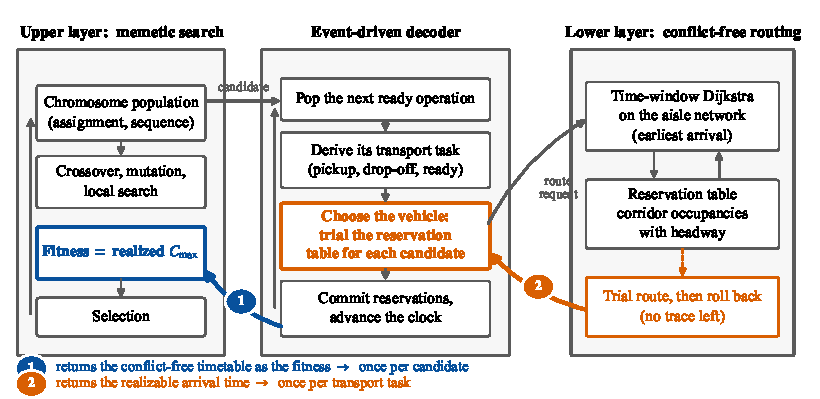
\includegraphics[width=\textwidth]{fig/fig_framework.pdf}
\caption{闭环双层框架。上层以 memetic 算法搜索指派与排序,下层以时间窗预约做无冲突路由,
中间的事件驱动解码器把上层的一个候选解翻译成一串运输任务。两条反馈通路以颜色区分且
\emph{进入上层的位置不同}:通路一(蓝,标记 1)把下层完成的无冲突时间表回传为适应度,每个
候选解触发一次;通路二(橙,标记 2)在选车之前查询预约表、取回实际可达的送达时刻,每个
运输任务触发一次,试探完毕即回滚,不在表上留下痕迹。第~\ref{sec:Chapter_V}~节的四级基线阶梯
所变化的正是这两条通路的有无。}
\Description{Schematic of the closed-loop bilevel framework: an upper memetic
search layer, an event-driven decoder, and a lower time-window reservation
routing layer, with two colour-coded feedback paths entering the upper layer at
different places---the evaluation path returning a realized makespan once per
candidate, and the decision path returning a realizable arrival time once per
transport task.}
\label{fig:framework}
\end{figure*}

\subsection{下层:时间窗预约与无冲突路由}
\label{sec:router}

\subsubsection{预约表}
唯一被争用的资源是走廊(假设 A6),因此预约表把每条走廊映射到一个按时间排序的半开占用区间
列表 $[t,\,t+\tau_e)$,每个区间标注占用它的车辆与任务。该表支持四种操作:查询不早于给定
时刻的最早可行进入时刻、提交一次占用、释放某个任务的全部占用,以及对整表做检查点与回滚。
节点不被预约:穿越节点耗时为零,而等待总是发生在停靠位上,假设 A6 已把停靠位与通行资源
分离。因此只需一种资源类型,这使路由器与那个独立的可行性校验器都保持简洁。

\subsubsection{时间窗 Dijkstra}
一段行驶用标签设定(label-setting)搜索来规划,其中标签 $(u,t)$ 表示"在时刻 $t$ 停在节点
$u$ 的停靠位上",其代价为 $t$(算法~\ref{alg:route})。松弛一条外出走廊时向预约表询问最早
进入时刻 $t'\ge t$,等待恰恰在此处产生:间隔 $t'-t$ 就是在 $u$ 的停靠位上耗掉的时间,
而 \eqref{eq:walk} 中的松弛量由搜索自身生成,不需要另行建模。在一次解码之内已提交的路径
不会被撤销,因此规划顺序就是解码器生成任务的顺序——即带有确定性优先级的优先级规划。

\begin{lem}[最早到达即充分]
\label{lem:label}
在每个节点上只保留最早到达时刻,即可得到相对当前预约表而言到达时刻最小的行驶段。
\end{lem}

\begin{proof}
停靠位容量充裕且不占用通行资源,因此一辆自时刻 $t$ 起停在 $u$ 的车,只需一直等到 $t'$,
便可复现任何在 $t'>t$ 到达 $u$ 的车所能采取的行为。于是到达时刻构成一个占优判据:更早的
标签绝不会更差。又因每次走廊松弛关于 $t$ 单调不减,该搜索是标签设定式的,目标节点第一次
被取出时即为最优。
\end{proof}

正是该引理使我们可以使用普通的 Dijkstra 标签,而不必采用安全区间规划的区间标签。它的脆弱
之处很有启发性:一旦引入第二个判据(例如为占用支付的价格),占优关系便不再是全序,从而被迫
改用多标签 Pareto 搜索。第~\ref{sec:interface}~小节会回到这一点,而它正是定价机制在同等
算力下失效的技术根源。

\begin{algorithm}[t]
\caption{\textsc{Route}:无冲突的单段路径规划}
\label{alg:route}
\small
\begin{algorithmic}[1]
\Require 起点 $s$、终点 $g$、最早出发时刻 $t_0$、预约表 $R$、是否提交标志 \textit{commit}
\Ensure 到达时刻,以及走廊占用区间的序列
\State 将标签 $(s,t_0)$ 压入以时间为键的优先队列
\While{队列非空}
  \State 弹出时间最小的标签 $(u,t)$
  \If{$u=g$} \State 回溯得到各占用区间;若 \textit{commit} 为真则逐一写入 $R$;
       \Return 到达时刻 $t$ \EndIf
  \ForAll{自 $u$ 外出的走廊 $e=(u,v)$}
    \State $t_{\text{in}} \gets R.\textsc{EarliestEntry}(e,t,\tau_e)$
       \Comment{在 $u$ 的停靠位等到 $t_{\text{in}}$}
    \State 松弛标签 $(v,\ t_{\text{in}}+\tau_e)$
  \EndFor
\EndWhile
\end{algorithmic}
\end{algorithm}

由于预约的数量有限、时间上有界,且 $G$ 强连通,路径总是存在的:最坏情况下车辆一直等到所有
既有占用全部过期,然后畅通行驶。这一观察使下文的命题~\ref{prop:decodable} 成立,也是无需
死锁修复的原因。单次调用的代价为 $O(|E|\,W\log|V|)$,其中 $W$ 为每条走廊上预约区间数的
均值。

对空表在所有取送节点对上运行同一搜索,即得到第~\ref{sec:Chapter_III}~节的无争用矩阵
$t^{*}$。它在三处被用到:开环配置中派车器的估计值、改派算子中的邻近项,以及两阶段基线的
运输时间。它同时是本章第~\ref{sec:speedup}~小节剪枝所依赖的可采纳下界。

\subsection{上层:编码与事件驱动解码}
\label{sec:upper}

\subsubsection{染色体编码}
设工序总数为 $N$,一个个体由两段构成:长度为 $N$ 的\emph{机器指派向量},其第 $k$ 个分量
在固定枚举下为第 $k$ 道工序取自 $\Omega_{ji}$ 的一台机械臂;以及\emph{工序序列},它是一个
可重排列,其中工件 $j$ 出现 $n_j$ 次,第 $x$ 次出现代表 $O_{jx}$。该序列是一个全局优先级
次序,共用同一台机械臂的工序之间的相对先后由它读出。

返回行程被折叠进同一表示。当 $\delta_{\mathrm{ret}}=1$ 时,每个工件额外贡献一次出现,对应
第~\ref{sec:Chapter_III}~节的伪工序,其机械臂固定为 $v_0$、加工时间为零。于是返回移动与普通
移动在同一条流中竞争车辆,并由同一段基因排序,解码器中不需要任何特例分支。

任务到车辆的指派\emph{有意}不编码,而是在解码过程中决定(第~\ref{sec:dispatch}~小节)。文献中
存在为它设置第三段基因的做法,但那会扩大搜索空间,并且放弃"任何染色体都可解码"这一保证,
从而不得不引入修复算子。

\subsubsection{事件驱动解码器}
解码器(算法~\ref{alg:decode})就是评价通路。它自左向右扫过工序序列,为每台机械臂维护其空闲
时刻,为每个工件维护其当前节点与就绪时刻,为每辆车维护其当前节点与可用时刻。当某道工序的
机械臂与工件当前位置不同时,便生成 \eqref{eq:tasks} 的运输任务,选定一辆车,并针对\emph{实时
的}预约表规划两段路径:到取货点的空载段与到目的地的满载段,两者由 \eqref{eq:load} 衔接。
随后工序按 \eqref{eq:bind} 开工,解码器同时记录两项中哪一项取到了最大值——即 \texttt{bind}
字段,后文全部归因都以它为依据。

\begin{algorithm}[t]
\caption{\textsc{Decode}:以完整无冲突仿真作为适应度}
\label{alg:decode}
\small
\begin{algorithmic}[1]
\Require 算例、路网、指派 $x$、工序序列
\Ensure 完工时间、时间表、逐走廊的让行统计量
\State 对所有机械臂置 $F_m\gets 0$;对所有工件置 $\mathrm{pos}_j\gets v_0$,
       $\mathrm{ready}_j\gets 0$
\State 对所有车辆置 $\mathrm{loc}_k\gets v_0$、$\mathrm{avail}_k\gets 0$;清空预约表
\ForAll{按序列次序取出的工序 $O_{ji}$(含伪工序)}
  \State $m\gets$ 在 $x$ 下 $O_{ji}$ 的机械臂;$d\gets \mathrm{loc}(m)$
  \If{$\mathrm{pos}_j=d$}
     \State $A_{ji}\gets \mathrm{ready}_j$ \Comment{同臂连续,不生成运输任务}
  \Else
     \State 选定车辆 $k$(第~\ref{sec:dispatch}~小节)
     \State $a^{\mathrm{E}}\gets\textsc{Route}(\mathrm{loc}_k,\mathrm{pos}_j,
            \mathrm{avail}_k)$;\ \ $\ell\gets\max(a^{\mathrm{E}},
            \mathrm{ready}_j)$
     \State $A_{ji}\gets\textsc{Route}(\mathrm{pos}_j,d,\ell)$;\ \
            $\mathrm{loc}_k\gets d$;\ \ $\mathrm{avail}_k\gets A_{ji}$
     \State 按走廊累计让行时间
  \EndIf
  \State 若 $F_m>A_{ji}$ 则 $\texttt{bind}\gets\texttt{machine}$,否则
         $\texttt{bind}\gets\texttt{arrive}$
  \State $S_{ji}\gets\max(A_{ji},F_m)$;\ \ $C_{ji}\gets S_{ji}+p_{ji}$;\ \
         $F_m\gets C_{ji}$;\ \ $\mathrm{pos}_j\gets d$;\ \
         $\mathrm{ready}_j\gets C_{ji}$
\EndFor
\State \Return $C_{\max}=\max_{j,i} C_{ji}$ 与时间表
\end{algorithmic}
\end{algorithm}

由此得到两条结构性性质。其一,预约是按扫描生成任务的次序做出的,因此一个染色体总是产出唯一
一张时间表:评价是确定性的,这正是第~\ref{sec:Chapter_V}~节同预算协议所依赖的前提。其二,
状态严格向前流动,因此一个只在位置 $x$ 之后扰动序列的邻居,会使 $x$ 之前的每个事件与每次
预约保持不变——这是增量式评价的基础;我们把它记为一项\emph{可用但当前实现未利用}的加速手段。

\begin{prop}[任何染色体都可解码]
\label{prop:decodable}
对任意指派与任意工序序列,算法~\ref{alg:decode} 均终止,并返回一张无冲突、无死锁且完工时间
有限的排程。修复算子永不被调用。
\end{prop}

\begin{proof}
由构造,序列是各前后约束链的一个拓扑序,因为工件的第 $x$ 次出现代表其第 $x$ 道工序;因此
$\mathrm{ready}_j$ 在被读取时总是已知的。缓冲区充裕(A4)意味着工序不会因无处存放而被阻塞,
故一旦物料到达,\eqref{eq:bind} 总给出有限的开工时刻。每次 \textsc{Route} 调用按
算法~\ref{alg:route} 之后的论证在有限时间内返回,且它只占用预约表报告为空闲的时窗,所以
\eqref{eq:excl} 由构造成立。扫描共执行 $N+n\delta_{\mathrm{ret}}$ 次迭代,每次在有限时刻上
安排有限多个事件。
\end{proof}

%% 原为 4.3 的一个子小节 "Dispatching",现提升为独立一节:它是本文承重的机制,
%% 不应埋在"上层编解码"之下。原 4.4 "What should cross the interface?" 的三种接口
%% 讨论降为本节的一个子小节,作为选定该机制的论证。
\subsection{预约表感知的车辆派遣}
\label{sec:dispatch}

在整个框架中,选车是唯一一处\emph{可以用估计代替事实}的地方,因此我们把它当作一个可闭合的
环节,而不是一个固定的设计。开环规则对每辆车打分
\begin{equation}
\label{eq:rule}
\mathrm{score}(k)=\max\bigl(\mathrm{avail}_k+t^{*}(\mathrm{loc}_k,\text{取货点}),\,
\mathrm{ready}_j\bigr)+t^{*}(\text{取货点},\text{目的地}),
\end{equation}
它从不查询预约表,因此可能选中一辆"在地图上很近、实际却被交通堵死"的车。这一规则并非我们
为了衬托而虚构的弱基线:它与文献~\cite{li2026framework} 所用的空闲优先规则同式。

作为默认配置的闭环变体改为\emph{试探}:对每个候选车辆,先\emph{带提交}地规划空载段,再
\emph{不提交}地规划满载段,记下真实送达时刻,然后把预约表整体回滚。空载段必须真实落表,
否则满载段看不到它占用的时窗,两段可能被规划到同一走廊的同一时段,从而给出一个在真实系统
中无法实现的乐观值。选定的车辆是实测送达时刻最早者,而非估计值最优者。

这一机制之所以奏效,有一个可以说清楚的理由,它也解释了为什么同样的思路用在\emph{选臂}上
收效甚微。AGV 之间是同构的(假设 A5),车与车唯一的差别就在于当前站位与路是否通得过;因此
选车是一个\emph{纯粹的拥堵决策},查询预约表所得到的信息可以全额兑现为目标函数的改善。而
选臂除了走廊差异之外还掺入了加工时长,后者往往压过前者,信息因而被稀释。

代价是显著的:试探把每个运输任务的路由调用数从 $2$ 抬到 $2N_A$,实测单次评价成本约为规则
派车的 \CostMultBefore{} 倍。若不加处理,这笔开销在同挂钟预算下会把机制带来的收益恰好吃光
——这正是第~\ref{sec:speedup}~小节存在的理由,也是第~\ref{sec:Chapter_V}~节只在同挂钟预算下
比较两者的原因。

\subsubsection{层间接口的三种选择}
\label{sec:interface}

两层既已固定,设计问题就变成\emph{下层应当回报什么}。共有三种答案,本文实现了全部三种,
并在同挂钟预算下逐一度量。上面的预约表试探属于第一种,也是唯一一种经得起该检验的;另外
两种的构造在此一并给出,度量结果见第~\ref{sec:Chapter_V}~节。

\paragraph{只回报时间。}
下层返回实现的时长,这正是评价通路已经在做的事,也是预约表试探所查询的东西。它使目标函数
正确,但不为搜索指方向:上层只知道某个解慢,不知道是哪个决策使它慢。在排产之后只路由一次的
方法甚至达不到这一点,因为它们只在决策固定之后知道一次真实时长。值得平实地指出这一选项本身
已经达成了什么,因为本文实测的收益主要归于它:搜索所比较的每一个候选解,都是按一个\emph{已
包含其自身交通所引起延误}的时长来排序的。

\paragraph{回报价格。}
与拉格朗日松弛及列生成中的协调机制相类比,自然的下一步是给被争用的资源定价:为每个
"走廊--时段"槽位附加一个影子价格 $\pi(e,b)$,让路由器在 Pareto 前沿上最小化
$\text{到达时刻}+\theta\cdot\text{价格}$,并让改派为它所需的通行权付费。我们完整实现了
这一方案——既包括一个扰动单个槽位容量并重解的定义式估计器,也包括一个每代刷新的廉价代理
——而在同等算力预算下它\emph{系统性地有害}。

这一机制值得写出来,因为它的失效原因可以推广。由争用造成的延误\emph{已经}被内部化了:让行的
车辆等待,该等待进入它自己的到达时刻,再经 \eqref{eq:bind} 传播进完工时间,并被适应度计入。
对占用者就同一次占用再收一次价格,等于把它数了两遍。于是车辆为了规避一笔\emph{已经支付过}的
代价而绕行或延迟出发,以承担一个一阶且确定的自身延误,去避免一个二阶且不确定的外部性。真正
残余的外部性只落在尚未被路由的任务上——扫描是有序的,早先的预约只可能妨碍其后的任务——而这
一部分同样已经体现在完整解码后的完工时间里。因此定价只增加扰动,不增加信息。这个推断是
\emph{架构层面}而非参数层面的:\emph{在任何以完整无冲突解码作为适应度的框架中,给下层目标
再加一个拥堵惩罚项,很可能是有害的。}

技术上还有第二重代价,它由引理~\ref{lem:label} 直接给出:一旦引入价格作为第二判据,到达时刻
不再是全序占优判据,单标签 Dijkstra 必须换成多标签 Pareto 搜索。无论最终是否真的收取价格,
这套机器都要付钱。第~\ref{sec:Chapter_V}~节的度量表明,击败定价的主要正是这笔开销,而非
上述双重计价的扰动本身。

\paragraph{回报冲突凭证。}
第三种选择是传递\emph{结构}。路由器在发生让行时知道走廊、时段以及占用者任务的身份;解码器
保留让行\emph{事件}而不只是它们的总量,因此该信息可以存活到评价结束。一份凭证就是三元组
(走廊,时段,对手任务),它被用来决定算子该触碰哪些工序。关键在于它\emph{不进入任何目标函数}:
下层依旧最小化到达时刻,上层依旧最小化完工时间,改变的只是邻域的\emph{构造方式}。既然没有
任何量被加入,也就没有任何量被数两遍——这避免了击沉定价的那个缺陷。第~\ref{sec:ls}~小节把它
落实为算子。它最终同样没有产出净收益:它构造出的邻域瞄得很准,但成功率过低,不足以抵偿它
消耗的解码次数。我们完整给出它,是因为"构造上站得住却依然不划算"的机制比只报告成功者更有
信息量——会自己设计出它的读者可以直接看到它的代价。

\subsection{降本:可采纳下界剪枝与胜者路径复用}
\label{sec:speedup}

上一小节的机制在同挂钟预算下面临一个具体的困境。按相同\emph{代数}比较,预约表试探比规则派车
好 \GainProbeSameGen{}(图~\ref{fig:protocols});但它单次评价贵 \CostMultBefore{} 倍,于是在
相同\emph{挂钟时间}下这一点增益恰好被它自己消耗的算力吃光,净效果几乎为零。换言之,在这个问题上\emph{降本就是增效}:只要能在不改变
任何选择结果的前提下压低成本倍数,机制的收益就能显现出来。本小节给出两项这样的优化,它们都
\emph{可证不改变输出}。

\paragraph{可采纳下界剪枝。}
关键观察是:无冲突路由只会因让行而\emph{更晚},绝不可能快过忽略争用的理想最短路。因此开环
规则所用的估计 \eqref{eq:rule} 恰好是实测送达时刻的一个\emph{可采纳下界}:
\begin{equation}
\label{eq:lb_dispatch}
\mathrm{lb}(k)=\max\bigl(\mathrm{avail}_k+t^{*}(\mathrm{loc}_k,\text{取货点}),\,
\mathrm{ready}_j\bigr)+t^{*}(\text{取货点},\text{目的地})\ \le\ \mathrm{est}(k),
\end{equation}
其中 $\mathrm{est}(k)$ 为对车辆 $k$ 做完整两段试探所得的实测送达时刻。于是,若某辆车的下界
已经不优于当前最优的\emph{实测}值,它的实测值必然也不优,便无需为它调用路由。被剪掉的车辆
一次路由调用也不产生。

\paragraph{胜者路径复用。}
试探结束后预约表被整体回滚,连胜者的两段路径也一并作废,随后解码器又把它们重算一遍,白白
浪费两次路由调用。而 $\textsc{Route}(\cdot,\textit{commit}=\text{真})$ 所做的不过是把各段
依次写入预约表,因此把胜者在试探阶段已算出的路径缓存下来、直接提交即可,无需重算。

\begin{prop}[两项优化保持输出不变]
\label{prop:speedup_equiv}
在按车辆编号升序扫描并保留首个\emph{严格}更优者的实现下,加入 \eqref{eq:lb_dispatch} 的剪枝
与胜者路径复用之后,所选车辆、所提交的预约以及最终时间表,与全量试探逐位相同。
\end{prop}

\begin{proof}
先看剪枝。设扫描到车辆 $k$ 时当前最优实测值为 $\mathrm{est}^{\ast}$。若
$\mathrm{lb}(k)\ge \mathrm{est}^{\ast}$,则由 \eqref{eq:lb_dispatch} 有
$\mathrm{est}(k)\ge\mathrm{lb}(k)\ge\mathrm{est}^{\ast}$,故 $k$ 不满足"严格更优"的替换条件,
在全量试探中同样不会成为胜者;跳过它不改变胜者。又因每次试探都以检查点开始、以回滚结束,
被跳过的试探对预约表不留任何痕迹,故也不改变后续任何一次查询的结果。再看复用:胜者的两段
路径是在同一张预约表状态下算出的,而回滚把表恢复到了试探开始前的状态,与解码器随后提交时
所面对的状态一致;由于 $\textsc{Route}(\cdot,\textit{commit}=\text{真})$ 仅把给定各段写入
预约表,提交缓存路径与重算后提交产生的占用区间完全相同。
\end{proof}

两项优化合计带来 \SpeedupProbe{} 倍加速,路由调用减少 \RouteCallCut{},把单次评价的成本倍数
从 \CostMultBefore{} 压到 \CostMultAfter{}。这不是工程细节,而是使第~\ref{sec:Chapter_V}~节
的正面结论得以成立的前提:在降本之前,同一机制在同挂钟下的净效果无法与噪声区分。

剪枝的效力本身依赖于车队规模,这一点须如实说明。下界越紧、越早出现一个好的现任值,被剪掉的
车辆就越多;而车队越大,候选越多,试探的总开销随 $N_A$ 线性增长。第~\ref{sec:Chapter_V}~节
给出实测的\emph{代价律}:剪枝的效力随车队增大而下降,但在我们测过的最大车队上仍然削减了
\RouteCallCutLo{} 的路由调用,因此它是效力衰减而非失效。这两个趋势合起来预言机制应当存在一个车队规模上的
适用上界;第~\ref{sec:whichcongestion}~小节说明为何现有的种子数尚不足以把这个上界定位出来。

\subsection{冲突制导局部搜索}
\label{sec:ls}

本小节把第~\ref{sec:interface}~小节的第三种接口落实为算子。每一代中,种群里最好的 $10\%$
接受局部搜索。需要提醒读者的是,这一机制在同挂钟预算下未能转为净收益
(第~\ref{sec:Chapter_V}~节);此处完整给出其构造,是为了让"为何最终选定预约表试探"这一取舍
有据可查。

\subsubsection{关键链的归因}
从取到完工时间的那个事件向后回溯可以得到一条链,但仅由工序构成的链无法说明一次开工\emph{为何}
迟到。当 $\texttt{bind}=\texttt{arrive}$ 时,该工序是在等物料,而成因可能是上游工序、可能是
无车可用、也可能是交通拥堵——三种情形对应三种完全不同的补救手段。因此我们把运输段也纳入回溯,
并给每一环打上标注(表~\ref{tab:attrib})。满载段上的让行一律记为走廊环,因为它直接延长了到达
时刻;空载段上则按让行时间占该段总耗时的比例、以 $0.5$ 为阈值,在"车辆"与"走廊"之间划分。

\begin{table}[t]
\caption{关键链各环的标注及其对应的补救算子。只有最后一类携带具体的走廊与时段,也只有它能
指名对手任务。}
\label{tab:attrib}
\footnotesize
\begin{tabular}{@{}llp{2.55cm}@{}}
\toprule
标注 & 判定条件 & 补救手段 \\
\midrule
\texttt{operation} & 一道真实工序正占用其机械臂 & --- \\
\texttt{machine} & $\texttt{bind}=\texttt{machine}$,被该臂上前一道工序阻塞
  & 重排序(通用变异) \\
\texttt{upstream} & 车辆先到,物料尚未就绪 & 递归至 $O_{j,i-1}$ \\
\texttt{vehicle} & 物料已就绪、车辆迟到,且延误中让行占比很小 & 更换车辆 \\
\texttt{corridor} & 在指定走廊、指定时段上发生让行 & 改派或错峰 \\
\bottomrule
\end{tabular}
\end{table}

从标注后的链上导出三类查询:链上的真实工序,改派算子从其中抽取候选;链上的"走廊--时段"槽位;
以及对给定走廊与时段,曾占用它并因而造成让行的那些任务——这才是凭证本身。

\subsubsection{两族算子}
拥堵有两种补救方向,框架为每一种提供一个算子。

\emph{改派改变"地点"。} 对关键链上至多 $L=5$ 道真实工序,为每个备选机械臂
$m'\in\Omega_{ji}\setminus\{m\}$ 打分
\begin{equation}
\label{eq:reassign}
\mathrm{score}(m')=t^{*}\bigl(\mathrm{pos}_{j,i-1},\mathrm{loc}(m')\bigr)
+t^{P}_{jim'},
\end{equation}
即一个邻近项与一个工时项之和,两者同为时间单位;得分最优的机械臂产生一个仅有单基因差异的
邻居。这两项恰好就是本文所讨论的那个权衡:更近的机械臂可能更慢,而 \eqref{eq:reassign} 正是
使搜索能够在"通往快速机械臂的路径被争用"时,用加工时间去买邻近性的那个式子。

该打分的一个早期版本还加上了 $\lambda$ 乘以候选机械臂处累计的让行时间。那一项是一个横跨整个
计划期与整个车队的总量,它随算例规模增长,而前两项始终停留在单道工序的尺度上;在一个 $240$
道工序的算例上它会支配整个打分,算子随之退化为"永远选最不拥堵的机械臂",从而毁掉它本要表达
的那个权衡。我们报告这一点,是因为 $\lambda$ 在不同算例之间不可比,对它做任何敏感性分析都将
是无意义的。

\emph{错峰改变"时间"。} 取链上最长的 \texttt{corridor} 环,向凭证查询在该时段占用过该走廊的
任务。由此得到两个有指向的邻居:把被阻塞的工序在序列中提前,使其移动被投放到一个更空闲的时窗;
或把\emph{单个}对手工序推后,使两者不再重合。每一轮只挪动一个对手,以保持邻域小而有针对性。
在序列中移动一次出现,是与\emph{另一个}工件的基因交换位置,因此工件内部次序自动得以保持,
结果仍是一个合法的可重排列;由命题~\ref{prop:decodable},它因而仍然可解码。

于是邻域最多包含 $L+2=7$ 个候选,且每一个都是由下层指名的。这正是它与通用变异算子的具体差别
——后者会在同一空间中均匀随机地抽样。

\subsubsection{接受准则}
第一个改进完工时间的邻居立即取代现任;随后从新的现任重新提取关键链,该轮重复,最多三轮。
某一轮若未产生任何改进则结束搜索(算法~\ref{alg:ls})。重新提取是必要的:一次成功的移动之后,
支配完工时间的那个成因通常会转移,因此若只在开始时算一次链,后续各轮就会去追一个已经不存在的
瓶颈。

\begin{algorithm}[t]
\caption{\textsc{ContentionGuidedSearch}:冲突制导的局部搜索}
\label{alg:ls}
\small
\begin{algorithmic}[1]
\Require 染色体 $c$ 及其解码结果 $r$
\For{$\textit{round}=1$ \textbf{到} $3$}
  \State $\mathcal{N}\gets\textsc{Reassign}(c,r)\ \cup\ \textsc{Stagger}(c,r)$
     \Comment{至多 $L+2$ 个邻居,均由凭证指名}
  \State \textit{improved} $\gets$ \textbf{假}
  \ForAll{$c'\in\mathcal{N}$}
    \State $r'\gets\textsc{Decode}(c')$
    \If{$r'.C_{\max}<r.C_{\max}$}
      \State $c\gets c'$;\ \ $r\gets r'$;\ \ \textit{improved} $\gets$
             \textbf{真};\ \ \textbf{跳出}
    \EndIf
  \EndFor
  \If{\textbf{非} \textit{improved}} \State \textbf{跳出} \EndIf
\EndFor
\State \Return $c,r$
\end{algorithmic}
\end{algorithm}

\subsection{外层遗传算法}

基于种群的这一层刻意保持常规,以使任何实测增益都可归因于上述机制而非算子调参。初始种群随机
生成——机械臂自 $\Omega_{ji}$ 均匀抽取,序列随机打乱——但另植入两个个体,一个把每道工序都指派
给其最快的机械臂,一个按负载均衡贪心指派。选择采用二元锦标赛并保留五个精英。交叉对序列段使用
保持前后约束的顺序交叉,对指派段使用均匀交叉;变异或交换序列中两个位置,或把一道工序移到另一
台可选机械臂。适应度即解码所得的完工时间。这些选择都是标准做法,不作为本文贡献。

%% 原标题 "Cost, and what is not claimed";"不主张什么"移到结论的局限小节。
\subsection{复杂度与代价分析}

一次适应度评价扫过 $N+n\delta_{\mathrm{ret}}$ 个事件;在闭环派遣下每次移动花费至多 $2N_A$ 次
路由调用,故每个个体为
$O\bigl((N+n)\,N_A\,|E|\,W\log|V|\bigr)$;开环规则以一个估计值为代价去掉了因子 $N_A$。
第~\ref{sec:speedup}~小节的下界剪枝不改变这一最坏情形界,但按命题~\ref{prop:speedup_equiv}
在不改变输出的前提下把实测的调用数降低了 \RouteCallCut{},即把因子 $N_A$ 换成了一个显著更小
的有效值。局部搜索则为它触碰的每个个体再增加至多 $3(L+2)$ 次解码。

其后果是,本框架内不同配置的成本相差达两个数量级。阶梯批次的实测每次评价为:开环配置
\MsOpen{}\,ms,闭环规则派车 \MsLoopRule{}\,ms,完整闭环 \MsLoopProbe{}\,ms,即闭环相对开环
约 $37$ 倍。定价档不在该批次内,它来自更早的定价扫描;在\emph{那一批内部},开启定价使单次
评价从 $15.05$\,ms 升到 \MsPriced{}\,ms,即再乘约 $4.8$ 倍。两批的绝对毫秒数不可直接相除,
但两个倍数相乘已足以说明跨度:最贵与最便宜的配置之间约两个数量级。因此按相同代数比较是没有
意义的,第~\ref{sec:Chapter_V}~节改为对齐挂钟时间。

这不是记账层面的细节,而是实验章围绕\emph{成本}而非围绕机制链来组织的原因。在固定预算下,
单次评价的成本与评价的次数是同一份资源的两种花法。一个机制只有在"它每次评价所增加的收益"
超过"它挤占掉的那些评价本可贡献的收益"时才配得上它的位置,而这是一个任何设计层面的推理都
无法预先判定的定量检验。本文的三个候选接口中,只有预约表试探通过了这一检验,且它只有在
第~\ref{sec:speedup}~小节的降本之后才通过。

最后是一个由框架结构本身引出的声明。交换乘子或价格的双层方案有时可以被证明收敛到不动点;
本框架不能,我们也不作此主张。下层是优先级式的而非联合最优的,上层是在非凸组合空间上的随机
搜索,而层间接口传递的是证据,不是一个可以充当 Lyapunov 函数的量。命题~\ref{prop:decodable}、
引理~\ref{lem:label} 与命题~\ref{prop:speedup_equiv} 所保证的东西更窄,但对一个启发式方法而言
更有用:搜索考察的每一个候选解都是可行的,其评价相对第~\ref{sec:Chapter_III}~节的冲突模型是
精确的,降本没有改变任何一个选择,并且整个过程是可复现的。解的质量是一个经验问题,由下一节在
一个为保持诚实而设计的协议下回答。

\section{实验与结果分析}
\label{sec:Chapter_V}

本章回答四个问题。把拥堵搬进搜索目标(闭环)本身值多少?预约表感知的派遣再值多少,它能否
代替闭环、二者是正交互还是近加性?这些收益在多大的算例范围内成立,以及\emph{以现有的种子数
能不能看清}它们在哪里成立?以及,那些我们实现了却未能转为净收益的更复杂接口,失效在哪一环?

\subsection{实验设置}
\label{sec:instances}

\subsubsection{受控算例族}
FJSP\_PT 基准的通行做法是把行驶时间给成一张"位置对--时长"矩阵,而这恰是本文要去掉的那条假设。
一张矩阵本身不足以定义车辆争用:争用发生在具体的通道上,而矩阵只记下端点之间的总时长。于是
问题不在于"矩阵够不够",而在于能否从矩阵反推出一张与之一致的通道网络。我们对实际取用的那一族
做了检验,答案是不能,而且理由比"文献没有附网络"更硬:
在 Homayouni 与 Fontes~\cite{homayouni2021production} 所用的 \PubNLayout{} 个布局中,
\PubNLayoutAsym{} 个矩阵\emph{全部不对称}(同一对位置往返时长不等,这是单向导轨的必然结果),
而其中 \PubNLayoutBad{} 个还\emph{违反三角不等式}——存在直达时长严格长于绕行时长的位置对。
这两条性质各自排除一种还原:本文的走廊是无向的、每条只有一个通行时间 $\tau_e$,故由它算出的
$t^{*}$ 必然对称,\PubNLayoutAsym{}/\PubNLayout{} 张矩阵因此都不可能是本文任何一张路网的
$t^{*}$;而任何图的全对最短路矩阵必然满足三角不等式,故那 \PubNLayoutBad{} 张矩阵\emph{根本不是
任何图的最短路闭包}——即便允许有向图也还原不出来。若强行为它们反推一张网络,得到的行驶时间
在那些位置对上必然\emph{严格更短}(绕行路径本身就成了更短路),那已经是\emph{另一个}算例,而
不再是文献发布并给出参考值的那一个,于是参考值也不再可比。因此我们生成一族受控算例,其中网络
是显式的,且
第~\ref{sec:features}~小节判定为关键的那些量可以逐个单独变化。这不排除在公开算例上做另一种
比较——把本文的争用约束删去、退化到与文献同一个数学问题上比对完工时间;
第~\ref{sec:external}~小节报告该比较,它标定的是上层搜索的强度,而非本文的框架。

全部算例共用同一核心:$12$ 个工件、每工件 $3$ 道工序共 $36$ 道真实工序、$8$ 台机械臂、
异质度 $H=0.3$,且运输与加工的时间尺度比 $\bar{T}_t/\bar{T}_p$ 标定到 $4.0$——即运输是
矛盾的主要方面,这正是本文问题设定的用意所在。在此核心之上变化三族因子
(表~\ref{tab:instances})。

\emph{A 族:布局(争用结构)}。五档 \texttt{funnel}、\texttt{high}、\texttt{mid}、
\texttt{low}、\texttt{scatter},通过改变网络容量而不改变行驶距离来调节争用:进入车间与
穿越车间的并行通道数逐档增加,每条通道是总时长相等的两跳路径,故增删一条只改变"多少辆车
能并行通过",不改变"任何东西要走多远"。节点与走廊数由 $13/12$ 递增到 $16/24$。其中
\texttt{funnel} 与 \texttt{high} 只差站台处的一条并行通道,即最小割减半,是本章最干净的
受控对照;\texttt{low} 与 \texttt{scatter} 网络规模相同,只差机械臂的空间摆放。

\emph{B 族:车臂比 $N_A/N_M$}。在 \texttt{funnel} 布局上取 $N_A\in\{4,8,12,16\}$,即车臂比
$0.5$、$1.0$、$1.5$、$2.0$,其中 $1.5$ 就是三族共用的基点(在表中以 \texttt{A funnel} 之名
列于 A 族)。这一族是为第~\ref{sec:costlaw}~小节的代价律准备的:派遣试探的开销随车队规模
线性增长,而剪枝的效力随之下降,两者的交叉点应当决定机制的适用上界。

\emph{C 族:柔性 $F$}。在同一布局上取 $F\in\{0.3,\,0.6,\,1.0\}$,即每道工序的可选机械臂
比例,其中 $0.6$ 同样是那个共用基点。柔性决定改派算子有多少可动的余地,也决定拥堵信息能在
多大程度上转化为指派上的调整。

三族共 $\NCases$ 个算例格:基点 \texttt{A funnel} 同时是 B 族的 $1.5$ 与 C 族的 $0.6$,
只生成、只运行一次,并在表~\ref{tab:instances} 与表~\ref{tab:bytag} 中只列一行。因此
$5+3+2=\NCases$,而 B 族与 C 族各自的扫描分别有四个和三个水平——
第~\ref{sec:whichcongestion}~小节读这两族时必须把基点那一格算进去,漏掉它会让扫描看上去比
实际单调。

\paragraph{这些取值落在公开算例的什么位置。}
算例既然自建,$H$、$F$ 与 $\bar{T}_t/\bar{T}_p$ 的取值就需要一个自身之外的依据,否则"参数
是我们定的"这一条无从回答。我们因此把第~\ref{sec:external}~小节所用的那 \PubNInst{} 个公开
算例用\emph{同一个}特征函数量了一遍——同一份代码、同一口径,故两边的数可以直接比,这是这组
对照能成立的前提。柔性的中位是 \PubFMed{},本章基点
$0.6$ 约为它的一倍半,而 C 族 $F=0.3$ 那一档正落在公开区间之内;异质度的中位只有 \PubHMed{},
\PubNInst{} 个算例中最大的一个也只有 \PubHMax{},即\emph{无一}达到本章共用的 $H=0.3$;时间尺度比
相差最远,公开算例的 $\bar{T}_t/\bar{T}_p$ 最高仅 \PubTtTpHi{},而本章标定到 $4.0$。

后两项都是外推,但性质不同,需分开交代。$\bar{T}_t/\bar{T}_p$ 那一项是\emph{有意为之},
且正是本文问题设定的前提:运输若只占加工时间的百分之几,它就不是矛盾的主要方面,车辆争用
也就不值得建模——通行的 FJSP\_PT 算例族恰好落在那一侧,这是本文另立算例的理由之一,而不是
取值失当。异质度那一项则是一处需要举证的外推:$H$ 若是收益的使能因子,把它定在文献区间之上
就会\emph{抬高}本章的主效应,那样各档之间的差值就有一部分是取值造出来的。这不能靠解释打消,
只能测。第~\ref{sec:whichcongestion}~小节用一批横跨四个 $H$ 水平的独立数据做了这个检验,
结论是收益并不随 $H$ 上升,且 $H$ 取在公开中位附近的那一档与取 $0.3$ 的那一档给出的增益几乎
相同;故这处外推没有把主效应抬高。我们把该检验放在那里而不是此处,是因为它需要先有增益的
定义才能读。

\begin{table}[t]
\caption{受控算例族。全部算例格共用 $12$ 工件、$36$ 道真实工序、$8$ 台机械臂、$H=0.3$、
$\bar{T}_t/\bar{T}_p\approx4.0$;三族分别只变化布局、车臂比与柔性。争用强度为初始随机种群
下让行时间占行驶总时间的比例,由算例自身结构决定而非人为设定。}
\label{tab:instances}
\small
%% 由 tab/gen_tables_ladder.py 生成:结构列直接由 tools/abc_matrix.py 的 build() 构造出
%% 算例后读出,下界调 algorithm/instance.py 的 simple_lower_bound,争用强度取自
%% baseline_ladder.csv 的 contention 列。任何一列都不是手打的。
%% generated by tab/gen_tables.py -- do not edit by hand
\begin{tabular}{@{}lccccrrl@{}}
\toprule
Structure & $|V|$ & $|E|$ & cut & far cut & $\varphi$ & LB & binding term \\
\midrule
\texttt{low} & 9 & 12 & 2 & 2 & 0.33 & 27.0--39.8 & job chain, machine load \\
\texttt{mid} & 11 & 12 & 2 & 2 & 0.29 & 25.0--44.8 & job chain, machine load \\
\texttt{high} & 10 & 10 & 2 & 1 & 0.29 & 25.0--44.8 & job chain, machine load \\
\texttt{funnel} & 9 & 8 & 1 & 1 & 0.29 & 25.0--44.8 & job chain, machine load \\
\bottomrule
\end{tabular}

\end{table}

\subsubsection{比较协议}
\label{sec:protocol}

这个设定下有三个陷阱会使朴素的比较近乎无意义。我们把协议写得较细,因为其中两个是我们先踩
进去、之后才改过来的。

\paragraph{统一执行器:报可实现的完工时间。}
这是公平性的支点,也是与文献比较时最容易出错的一处。开环方法在忽略争用的前提下排产,它自己
报出的完工时间在真实系统里\emph{根本不可行}。因此本章的所有配置,无论计划从哪里来,都必须
放进\emph{同一个}无冲突路由器里执行、过\emph{同一个}独立校验器,报告的一律是执行后可实现的
完工时间。这一步不是形式主义:开环计划的乐观幅度恰等于该算例的争用强度,在漏斗算例上可达
\ContentionHi{}。若允许各方各报自己口径下的数,比较立即失去意义,而被比较的一方会凭一个
不可实现的数字胜出。

\paragraph{同挂钟,而非同代数。}
各配置评价的\emph{不是同一个对象}。开环配置的一次评价是查常数矩阵 $t^{*}$ 的解码;闭环配置
要对每个候选做完整的无冲突路由;定价变体还要额外跑多标签搜索。实测单次评价成本跨越两个数量
级。因此按相同代数比较等于给昂贵的配置多送几十倍算力,一个看似的机制增益可能只是预算更大。
我们改为对齐挂钟时间:各配置在同一算例上共享同一预算,早停阈值放宽以确保预算被真正用尽,
每次运行都报告它是耗尽预算还是提前收敛。

对齐时间同样不是中性的——它反过来给便宜的配置多送几十倍搜索次数。因此两种口径都不能单独
呈现。我们为每个配置同时报告单次评价成本与实际完成的评价次数,使搜索努力的差异可见而非
被藏起来,并在第~\ref{sec:costlaw}~小节把这一"成本与次数的兑换率"本身作为对象来测。

\paragraph{足够的种子与配对检验。}
本问题中单种子读数是没有价值的:在同一算例上,\emph{同一}配置的三个种子之间我们观察到过
$11$ 个完工时间单位的极差,超过我们所度量的任何机制效应。因此每格跑 $\NSeeds$ 个种子,每个
比较都按种子配对,并用双侧 Wilcoxon 符号秩检验。配对按显式键 $(\text{算例},\text{种子})$
形成,而非按列表位置——这个区别在某格数据不全时是决定性的。需要预先说明这一选择的代价:
$\NSeeds$ 个种子足以在 $\NPairs$ 个配对的合计口径上分辨数个百分点的效应,却\emph{不}足以在
单格内分辨它。第~\ref{sec:whichcongestion}~小节会显示这个界限恰好横在本文两个机制之间,
而我们把逐格结论限制在它之内。

\paragraph{正确性。}
每个解都由一个独立于解码器的校验器重新检查,该校验器从时间表出发重新推导走廊占用,并与算例的
复合下界比对。未过校验或低于下界的运行单独报告,绝不并入任何格的均值。每次完成的运行都追加
写入账本并落盘,故中断的批次可以续跑而不重算,报表也从账本而非内存重建。

\subsubsection{实现与运行环境}
实验在 Intel Xeon W-1270 @ $3.40$\,GHz 上单线程运行;实现为纯 Python,不依赖任何求解器。
因此绝对耗时不能与编译型实现相比,这一点对协议是有影响的:更快的实现会让\emph{每一个}配置
在同一预算内做更多次评价。但它不会改变各比较所依赖的"成本与评价次数之间的兑换率",因为该比率
是在共享同一实现的配置之间测得的。

\subsection{四级基线阶梯}
\label{sec:arms}

一体化调度类工作的实验最常见的失误,是把两个不同的问题混成一个数字来报:\emph{与文献相比
好多少},以及\emph{我们自己的哪个部件贡献了多少}。前者要求与已发表方法的\emph{结构}对齐,
后者要求只动一个部件。只报消融会低估问题的分量,只报文献比较则会把无冲突路由本身的价值
冒领成本文的创新。我们因此把它拆成一道四级阶梯,每一级都对应一个可指名的结构。

\begin{description}[leftmargin=0pt,topsep=3pt,itemsep=3pt]
\item[B0:开环规划 + 真实执行。] 上层在理想最短路上搜索(即搜索时不计冲突),搜完把计划
放进真实路由器执行。这是~\cite{li2026framework} 的忠实模型:其调度层产出忽略运输争用的
甘特图,下游用优先级路由解冲突,再把到达时刻平移回时间轴;其派车用空闲优先规则
$k^{*}=\arg\min \text{Cost}(\text{path}_k,L_{\text{start}})$,与本框架的规则派车
\eqref{eq:rule} 同式。
\item[B0+:开环规划 + 预约表感知派车。] 排产同样冻结,只把车辆指派改为查预约表决定。这是
~\cite{sun2023integrated} 两阶段结构的对应物:其第一阶段的混合遗传算法在\emph{常数运输时间
矩阵}上排产,第二阶段才在冻结的排产上优化车辆指派并处理冲突,无回流。此处以试探派车作其
第二阶段的贪心近似——试探未必弱于对方的遗传算法,故这一级是对基线\emph{宽容}的口径。
\item[B1:闭环规划 + 规则派车。] 搜索时即计冲突,派车仍用理想矩阵估计。与 B2 信息完全对等。
\item[B2:闭环规划 + 预约表感知派车。] 本文方法。
\end{description}

这四级不是一条链,而是一个 $2\times 2$ 析因:因子一为"拥堵是否进入搜索目标"(开环/闭环),
因子二为"派车是否查预约表"(规则/试探)。按析因而非按链来组织是必要的,因为链上相邻两行
只有在此前每个因子都被固定时才只差一个因子;一旦两行差了两个因子,它们的差值就不可解释。
具体地,$\text{B0+}\to\text{B1}$ 同时跨越两个因子,\textbf{不能}用来度量闭环的价值——我们
把它列出仅为对账。干净的对比是固定一个因子只动另一个,即表~\ref{tab:arms} 的四格之间的
四个配对。

\begin{table}[t]
\caption{四级阶梯作为 $2\times 2$ 析因。行为"拥堵是否进入搜索目标",列为"派车是否查预约表"。
四格中只有沿同一行或同一列的比较是单因子的,对角比较跨两个因子、不可用于归因。}
\label{tab:arms}
\footnotesize
\begin{tabular}{@{}lcc@{}}
\toprule
 & 规则派车 & 预约表感知派车 \\
\midrule
开环规划(排产冻结) & B0~\cite{li2026framework} & B0+~\cite{sun2023integrated} \\
闭环规划(拥堵入目标) & B1 & \textbf{B2}(本文) \\
\bottomrule
\end{tabular}
\end{table}

B0 的执行口径需要交代,因为它直接影响基线的强弱。开环搜出的计划本身含有一套派车决策,执行时
有两种复现方式:\emph{复现计划}用原计划逐字指定的车辆,即"计划怎么定就怎么执行";\emph{现场
改派}在执行时按规则重新派车。实测前者更强(漏斗算例上 $63.00$ 对 $78.00$),且它才是
~\cite{li2026framework} 的忠实模型——该文的任务分配层在甘特图上先定好机器人,执行滑坡时
只平移时间轴、不改派。因此我们取\emph{较强}的那一个作为主报口径,另一个一并给出以示我们
没有挑对自己有利的那个。对基线取强者,是举证责任应当由我们承担的部分。

\subsection{主结果}
\label{sec:main}

表~\ref{tab:main} 给出四级阶梯在 $\NCases$ 个算例格 $\times$ $\NSeeds$ 个种子、共
$\NPairs$ 个配对下的结果,每格同挂钟预算,全部运行均通过独立校验。以下三段分别读出析因的
两个主效应与端到端的合计。

\begin{table}[t]
\caption{四级阶梯在同挂钟预算下的完工时间,以及 $2\times 2$ 析因的四个单因子配对比较。
负值表示完工时间下降,即更好。$n=\NPairs$ 个按 $(\text{算例},\text{种子})$ 配对的比较,
双侧 Wilcoxon 符号秩检验。}
\label{tab:main}
\small
%% 由 tab/gen_tables_ladder.py 从 clbs/output/baseline_ladder.csv 生成。该脚本同时打印
%% 导言区的整块宏定义,故表与正文的数字必然同源:重跑实验后只需重跑脚本、贴一次宏。
%% 已核实脚本独立复现出导言区当前的全部数值(增益、p 值、胜负计数、争用区间)。
%% 由 tab/gen_tables_ladder.py 生成,请勿手工编辑
%% 数据源:clbs/output/baseline_ladder.csv 等,见脚本首部
\begin{tabular}{@{}lrrrrr@{}}
\toprule
算例 & 争用强度 & B0 & B0$^{+}$ & B1 & \textbf{B2} \\
\midrule
A funnel & 31.9\% & 58.10 & 53.50 & 44.70 & \textbf{42.40} \\
A high & 30.9\% & 56.00 & 51.40 & 39.90 & \textbf{37.70} \\
A low & 11.8\% & 64.50 & 64.60 & 57.80 & \textbf{57.10} \\
A mid & 10.8\% & 46.40 & 42.70 & 39.40 & \textbf{37.40} \\
A scatter & 6.6\% & 62.30 & 62.30 & 57.20 & \textbf{57.10} \\
\midrule
B NA/NM 0.5 & 15.8\% & 71.00 & 70.50 & 69.00 & \textbf{65.10} \\
B NA/NM 1.0 & 30.2\% & 56.70 & 56.50 & 47.50 & \textbf{49.80} \\
B NA/NM 2.0 & 32.4\% & 70.60 & 64.20 & 42.20 & \textbf{44.20} \\
\midrule
C F=0.3 & 27.7\% & 74.30 & 69.50 & 51.60 & \textbf{47.30} \\
C F=1.0 & 33.5\% & 52.10 & 47.50 & 39.30 & \textbf{36.30} \\
\midrule
\emph{全体均值} & --- & 61.20 & 58.27 & 48.86 & \textbf{47.44} \\
\bottomrule
\end{tabular}

\vspace{0.6em}

\begin{tabular}{@{}lrrr@{}}
\toprule
单因子配对对比 & $\Delta C_{\max}$ & 胜/负/平 & $p$ \\
\midrule
闭环的价值(规则派车下) & $-18.86\%^{***}$ & 96/2/2 & $<10^{-4}$ \\
闭环的价值(试探派车下) & $-17.75\%^{***}$ & 93/5/2 & $<10^{-4}$ \\
试探派车的价值(开环下) & $-4.59\%^{***}$ & 68/19/13 & $<10^{-4}$ \\
试探派车的价值(闭环内) & $-2.45\%^{**}$ & 60/34/6 & $0.0054$ \\
\midrule
\textbf{端到端:文献结构 $\rightarrow$ 本文} & $-21.35\%^{***}$ & 94/5/1 & $<10^{-4}$ \\
\bottomrule
\end{tabular}

\end{table}

\paragraph{闭环本身的价值。}
固定派车方式、只改变"拥堵是否进入搜索目标",闭环在两种派车方式下都显著更优:规则派车下
$\text{B0}\to\text{B1}$ 为 $-\GainLoopRule$($p=\PLoopRule$),试探派车下
$\text{B0+}\to\text{B2}$ 为 $-\GainLoopProbe$($p=\PLoopProbe$)。这个增益不能归因于搜索
努力,因为比较方向恰恰相反:开环配置的一次评价只需查常数矩阵,在同一预算内能完成数倍于闭环
的评价次数。它搜得更狠却仍然输,原因是它在优化一个错误的目标,只有当决策已被冻结之后才发现
真实的运输代价。图~\ref{fig:convergence} 在单个算例上把这一差距画了出来。

值得指出这一级差距的归属。把拥堵搬进搜索目标是本文的主张,同时也是~\cite{li2026framework}
在其结论中自陈的未来工作("extending this mechanism into a fully iterative loop"),因此
可以正当主张;但它必须与下一段的机制贡献\emph{分开}报,不得合并成一个数字。

\begin{figure}[t]
\centering
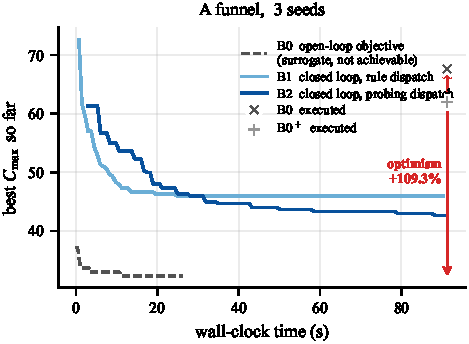
\includegraphics[width=\columnwidth]{fig/fig_convergence_closedloop.pdf}
\Description{Best-so-far makespan against wall-clock time for the ladder
configurations, with the open-loop curve marked as a surrogate objective and its
realizable value shown as a separate point.}
\caption{单个 \texttt{funnel} 算例上的收敛曲线,横轴为挂钟时间,曲线为多种子的逐时刻均值。
实线(B1、B2)自始至终画的都是可实现的完工时间;虚线是开环搜索\emph{自己的}代理目标,即它
实际在优化的东西,而叉号与十字标出同一份计划经无冲突路由执行后落在哪里。虚线终点与叉号之间
的落差即该算例的乐观幅度,也是"在环内评价"这一步的全部理由:开环并非收敛得不好,而是收敛到
了一个不存在的位置。}
\label{fig:convergence}
%% 由 fig/fig_convergence.py 生成(输出名 fig_convergence_closedloop,勿改,正文已引用),
%% 数据源 clbs/output/ladder_convergence.csv 与 ladder_cost.csv,由 tools/ladder_diag.py 落盘。
%% 该图是说明性的:它画形状与落差,不承载统计主张,故只取三算例三种子,正文统计一律以
%% baseline_ladder.csv 为准。此口径已写在 ladder_diag.py 的首部注释里。
\end{figure}

\paragraph{预约表感知派遣的价值。}
固定闭环与否、只改变派车决策,得到本文机制自身的贡献。在\emph{闭环内部},
$\text{B1}\to\text{B2}$ 为 $-\GainProbeLoop$($p=\PProbeLoop$)。这一级的两档信息完全对等
——同样的排产搜索、同样的预算,唯一差别是选车时是否查预约表——因此它是本文承重机制的干净
度量。但它是一个\emph{合计}口径的度量:该效应在 $\NPairs$ 个配对上显著,而逐格只有
\CellsSigProbe{} 格自身达到显著,其余各格(含全部四个车臂比水平)与零不可区分。因此
$-\GainProbeLoop$ 应读作"在本算例族上平均为正",不是一个可以逐格兑现的点估计;
第~\ref{sec:whichcongestion}~小节说明这一分辨率限制的后果。

在\emph{开环之下},同一个机制值 $-\GainProbeOpen$($p=\PProbeOpen$),同样显著。开环试探
并不"几乎不值钱";它就是~\cite{sun2023integrated} 两阶段结构相对~\cite{li2026framework}
忠实开环的那一段进步。但它的量级(\GainProbeOpen{})远小于闭环主效应(\GainLoopRule{}),
这才是下一小节要钉死的判断。

\paragraph{端到端。}
从文献结构到本文方法,$\text{B0}\to\text{B2}$ 合计 $-\GainEndToEnd$
($p=\PEndToEnd$,$\WinEndToEnd$ 胜 $\LoseEndToEnd$ 负)。这是一个可以正当主张的端到端数字,
前提是它被拆开报告过——上面两段就是那个拆解。

\subsection{主效应、次效应与不可替代性}
\label{sec:complement}

上一小节留下的不是"开环试探不显著",而是一个\emph{量级}问题:开环试探显著但小
($\GainProbeOpen$),闭环显著且大($\GainLoopRule$),闭环内试探的平均被大车队两格拖成
$\GainProbeLoop$。本小节用析因把"可否互相替代"与"是否正交互"分开回答。

\paragraph{交互的定量判据。}
若闭环与派遣两个因子彼此独立,端到端增益应恰为两者单独增益的复合,即
$\GainIndepProduct$。实测为 $\GainEndToEnd$,略低于独立预测——\emph{无正交互},呈近加性
或略亚加性。这一点一并说明了本文\emph{不}主张什么:两个机制不是彼此放大的,把它们叠在
一起得到的就是它们各自贡献之和减去一点点。

\paragraph{不可替代,而非必须捆绑。}
真正站得住的主张不是"两者必须一起用才有效",而是"开环试探不能代替闭环"。把拥堵感知
的派车装在冻结排产上,最多拿到约 $\GainProbeOpen$;把拥堵搬进搜索目标,即使仍用规则派车,
也能拿到约 $\GainLoopRule$。熟悉~\cite{sun2023integrated} 的审稿人若问"你们的派车机制
装在两阶段框架里是不是也一样管用",答案是:管用,但只管用到开环试探那一档;要拿到本文这一级
的改善,拥堵必须在\emph{搜索时}进入目标。B2 仍是端到端最优,因为它把主效应与次效应叠在
一起,而不是因为存在一个把两者焊死的正交互项。

\paragraph{对文献的含义。}
因此"先排产、后解冲突"路线的问题,不在于第二阶段的派车做得不够好——第二阶段在我们的
口径下确实有 $\GainProbeOpen$ 的显著收益——而在于它把主效应留在了桌面上。第二阶段能挽回
的东西有一个由第一阶段无知所框定的上界;要突破这个上界,必须把无冲突执行放进适应度。

%% 原此处的 fig:protocol(评价成本与评价次数)与 fig:protocols(两种预算口径下的
%% 同一组比较)已移到第 5.7 小节"代价律与降本效果"——它们说明的是成本与次数的兑换率,
%% 属于代价分析而非主结果。

%% 原标题 "Which congestion is worth feeding back?" 同为问句,改为正面表述。
%% 原副题"适用区间"已撤:逐格显著性表明本文的种子数不足以定位任何区间,
%% 见下文"能看清什么"一段。这一撤回是 2026-08-16 复核逐格 p 值后作出的。
\subsection{逐因子族的稳健性,以及逐格分辨率的限度}
\label{sec:whichcongestion}

主结果是在 $\NCases$ 个算例格上汇总的。本小节把它按三个因子族拆开。原本的意图是划出机制的
适用区间——一个只在特定结构上成立的收益,若不说明边界,读者无法判断它是否适用于自己的场景。
拆开之后我们发现,这个意图对两个效应中的一个可以达成,对另一个不能,而这个不对称本身就是
本小节要报告的东西。三族分别检验三个可以事先说清的预期。

\emph{布局(A 族)}检验收益是否随争用强度增长。这是最直接的预期:闭环与预约表试探处理的都是
争用,若争用本身很弱,两者都无从发挥。\texttt{funnel} 与 \texttt{high} 只差站台处一条并行
通道,即最小割减半,是其中最干净的受控对照。

\emph{车臂比(B 族)}检验\emph{上界}。派遣试探的开销随车队规模线性增长,而
第~\ref{sec:speedup}~小节的剪枝效力随车队增大而下降(等价性自检中最大车队一档的调用削减率
最低)。因此应当存在一个车队规模,超过它之后机制的收益会被自身开销吞掉。该族取四个水平
$N_A/N_M\in\{0.5,1.0,1.5,2.0\}$,其中 $1.5$ 即共用基点 \texttt{A funnel}。

\emph{柔性(C 族)}检验机制是否依赖指派上的可动余地。柔性越高,同一道工序的可选机械臂越多,
拥堵信息越有机会转化为指派调整。该族取三个水平 $F\in\{0.3,0.6,1.0\}$,其中 $0.6$ 同为基点。

\paragraph{能看清什么:两个效应的逐格分辨率相差悬殊。}
在读任何一族之前必须先看表~\ref{tab:bytag} 的显著性标记,因为它决定了哪些逐格叙述是允许的。
闭环效应在 \CellsSigLoop{} 个格上自身即达显著,唯一的例外是车队最紧的一格
($\text{B0}\to\text{B1}$ 为 \GainLoopStarve{},不显著);因此按族解读它的走势是有依据的。
闭环内的试探效应则只在 \CellsSigProbe{} 个格上显著,即 C 族的两格;其余八格——包括全部四个
车臂比水平——都与零不可区分。这与第~\ref{sec:protocol}~小节所述的种子间离散度是一致的:
该效应的量级(数个百分点)与单格 \NSeeds{} 个种子所能分辨的下限是同一个数量级,合计
$\NPairs$ 个配对才把它抬出噪声。据此,下文对 A、B 两族的试探读数一律只作\emph{方向性}描述,
不作结论;凡涉及符号的判断只在 C 族与合计口径上给出。

\begin{table}[t]
\caption{逐算例格的四级阶梯结果与两个主效应,按三个因子族分组($n=\NSeeds$ 个按种子配对的
比较每格;$^{*}p<0.05$,$^{**}p<0.01$)。争用强度由算例结构决定,一并列出以便判断收益是否
随其变化。负值表示完工时间下降。两个增益列与表~\ref{tab:main} 用同一个估计量,即逐对相对
增益在种子上的均值,因此十格的均值精确等于表~\ref{tab:main} 的合计值;代价是该列不能由
同一行的两个均值列相除反推。\texttt{A funnel} 一行同时是 B 族的 $N_A/N_M=1.5$ 与 C 族的
$F=0.6$,只运行一次,故只列一行。}
\label{tab:bytag}
\small
%% 由 tab/gen_tables_ladder.py 生成,按 A/B/C 三族分块。
%% 逐格增益列已于 2026-08-16 从"两档均值之比"改为"逐对相对增益的均值",与 tab_main 及
%% 导言区宏同源;同时加印显著性标记,因为下文按格读符号。
%% generated by tab/gen_tables.py -- do not edit by hand
\begin{tabular}{@{}lccccc@{}}
\toprule
& \multicolumn{4}{c}{$\Delta C_{\max}$ (\%) at $H=$} & pooled \\
\cmidrule(lr){2-5}
Structure & $0$ & $0.15$ & $0.3$ & $0.5$ & (\%) \\
\midrule
\texttt{low} & $+10.3$ & $+5.6$ & $+8.8$ & $+10.4$ & $+8.76^{***}$ \\
\texttt{mid} & $+3.3$ & $+4.0$ & $+4.5$ & $+4.3$ & $+4.03^{***}$ \\
\texttt{high} & $+11.3$ & $+8.1$ & $+10.7$ & $+7.9$ & $+9.50^{***}$ \\
\texttt{funnel} & $+9.2$ & $+8.7$ & $+9.4$ & $+6.5$ & $+8.47^{***}$ \\
\bottomrule
\end{tabular}

\end{table}

\begin{figure}[t]
\centering
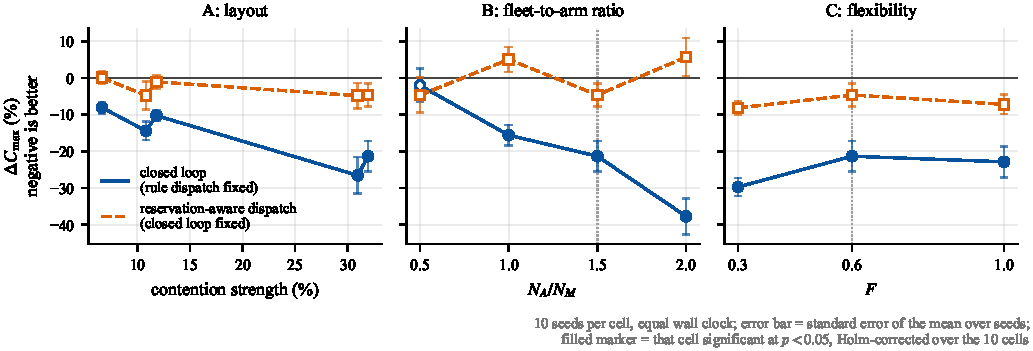
\includegraphics[width=\columnwidth]{fig/fig_prediction3.pdf}
\Description{Three panels of line plots: closed-loop gain and probing-dispatch
gain across layout (vs contention), fleet-to-arm ratio, and flexibility. The
closed-loop curve is significant at nearly every cell; the probing curve is
hollow-marked at the cells where it is not significant, which is most of them,
and its sign alternates across the four fleet-ratio levels.}
\caption{两个主效应在三个因子族上的分布。左:布局族,横轴为争用强度;中:车臂比族,横轴为
$N_A/N_M$;右:柔性族。B 与 C 两族含共用基点(空心竖线所在的 $1.5$ 与 $0.6$),它同时列于
A 族的 \texttt{A funnel}。实心标记为该格自身显著($p<0.05$),空心为不显著。闭环增益几乎
处处显著且大体随争用上升;试探增益只在柔性族两端显著,在车臂比族的四个水平上符号交替、
无一显著——因此本图要读的是两条曲线\emph{可信度}的差别,而不是试探那条曲线的形状。}
\label{fig:prediction3}
%% 由 fig/fig_prediction3.py 从 clbs/output/baseline_ladder.csv 生成。横轴:A 族取争用强度
%% (布局族没有自然的数值水平,而布局操纵改变的正是争用),B/C 族取算例名末尾的因子水平——
%% 那个数字由 tools/abc_matrix.py 生成算例时写入,故按构造即为水平本身;基点 A funnel 的
%% 名字里没有水平,其 (1.5, 0.6) 由脚本按 abc_matrix.BASE 显式补入,见脚本内注释。
%% 标记的实心/空心由逐格 Wilcoxon 的 p 值决定。上一版按增益是否为正标注 "harmful",
%% 那等于把不显著的符号当成结论,现已改为按显著性区分标记。
\end{figure}

表~\ref{tab:bytag} 与图~\ref{fig:prediction3} 给出逐格结果。三族的读法各不相同,须分开说。

\emph{布局族。}闭环增益随争用强度大体上升,且五格逐格皆显著:最不拥堵的 \texttt{scatter}
(争用 \ContentionLo{})上 $\text{B0}\to\text{B1}$ 为 $-8.1\%$,中等的
\texttt{mid}/\texttt{low} 为 $-14.4\%$/$-10.3\%$,最拥堵的 \texttt{funnel}/\texttt{high} 达
$-21.3\%$/$-26.6\%$。"大体"这个限定词是必要的:五格里有两处逆序,\texttt{mid} 的争用低于
\texttt{low} 却收益更大,\texttt{funnel} 的争用高于 \texttt{high} 却收益更小,而后一对恰是
我们指定的最干净受控对照。因此可以主张的是量级上的联系——两端相差约三倍,最拥堵一格
$-26.6\%$ 对最不拥堵一格 $-8.1\%$——而不是争用强度对收益的单调排序。争用强度是一个粗糙的一维摘要,它把"拥堵有多少"
压成一个数,却不区分其中有多少是指派可以绕开的;第~\ref{sec:limitations}~节把这一点列为
局限。试探增益在本族逐格皆不显著,故只记录其方向:五格中四格为负,与闭环同向。

\emph{车臂比族。}这是我们原本打算钉死适用上界的地方,而实测结果是这个上界钉不下来。四个
水平上闭环内试探依次为 $-\GainProbeStarve$($N_A/N_M=0.5$)、\GainProbeFleetOne{}($1.0$)、
\GainProbeFleetBase{}($1.5$,即基点 \texttt{A funnel})、\GainProbeFleetTwo{}($2.0$):符号
交替,不单调,且四格无一显著($p$ 分别为 $0.4121$、$0.2011$、$0.1386$、$0.3313$)。若只取
$0.5$、$1.0$、$2.0$ 三格,曲线看上去正是代价律所预言的那条单调上升线,我们的前一版稿件也
确实据此写下了"$N_A/N_M\ge 1$ 即为适用上界";把夹在中间的基点补回去之后,这条叙事不成立。
我们保留这段记述而不是径直删去,因为它说明了一件方法层面的事:当一个效应的量级与逐格噪声
相当时,\emph{子集的选取本身就足以造出一条趋势},而防住它的不是更好的解释,是把扫描补全
并逐格检验。代价律(第~\ref{sec:costlaw}~小节)所预言的上界因此仍是一个未被检验的预言——
要检验它需要把种子数提高到足以分辨数个百分点的量级,这超出本文的算力预算。
闭环本身在本族上则清晰得多:$1.0$ 与 $2.0$ 两格分别为 $-15.6\%$ 与 $-37.7\%$,均显著,
说明车队变大主要改变的是闭环能捞回多少,而不是试探。

\emph{柔性族。}这是试探效应唯一逐格显著的一族,也因此是唯一能作结论的一族:
$F=0.3$、$0.6$、$1.0$ 三个水平上分别为 $-8.2\%$、\GainProbeFleetBase{} 与 $-7.2\%$,
两端显著、中间基点不显著,三者量级接近且同号。拥堵信息主要经由派车与时序兑现,并不强依赖
"还有没有另一台臂可改派"。这对机制解释是利好:它不是柔性车间专属的旁路,在指派余地受限时
仍然成立。闭环增益在本族同为大幅负值且显著。

\paragraph{来自另一批自建算例的独立印证。}
上述结论建立在一个算例族与一个基线口径之上,因此我们用一批独立的数据交叉核对。该批次仍是
带争用的自建算例(公开基准上的另一种比较见第~\ref{sec:external}~小节,那里争用已被删去),为
\MatrixCells{} 个算例格 $\times$ $10$ 种子、同挂钟预算、共 \MatrixRuns{} 次运行,算例核心与
基线口径都与本章不同——它以两阶段代理运输作为基线,并在四个争用族与四个异质度水平上交叉。其
\emph{集成增益}(两阶段 $\to$ 闭环)为 \GainIntegMatrix{},\MatrixCells{} 格中
\SigIntegMatrix{} 格显著,区间 \GainIntegMatrixLo{} 到 \GainIntegMatrixHi{}。这与本章闭环主
效应的方向与量级一致,且是在不同算例、不同基线下得到的,故可作为稳健性的独立证据。

\paragraph{异质度不是收益的放大器。}
这批数据的四个异质度水平正好回答第~\ref{sec:instances}~小节留下的那个问题。按 $H$ 把
\MatrixCells{} 格分成四组(每组 $4$ 格,即四个争用族各一格),集成增益依次为:$H=0$ 时
\GainIntegHZero{},$H=0.15$(实测 \MatrixHMeasLow{})时 \GainIntegHLow{},$H=0.3$ 时
\GainIntegHMid{},$H=0.5$ 时 \GainIntegHHigh{};\MatrixCells{} 格上增益与 $H$ 的秩相关为
弱负的 \RhoIntegH{}。有三件事要从这里读出来。

其一,取值外推那一问就此答复:实测 $H=\MatrixHMeasLow$ 一档恰落在公开算例的中位 \PubHMed{}
附近,而它给出的 \GainIntegHLow{} 与本章基点 $H=0.3$ 那一档的 \GainIntegHMid{} 相差不到半个
百分点。把 $H$ 定在文献区间之上,并没有抬高闭环的主效应。

其二,我们原本预期收益随 $H$ 上升,这条预期\emph{不成立}——趋势非单调,秩相关为负。但这里
必须守住本小节前面反复强调的那条纪律:四组各只有 $4$ 格,而逐格增益
的散布(\GainIntegMatrixLo{} 到 \GainIntegMatrixHi{})远大于四组均值之间的差距,故本批数据
支撑得起的只有"收益不随 $H$ 上升"这一条否定式,而\emph{不足以}断言 $H=0.5$ 那一档真的更低。
就否定式本身我们给一个与第~\ref{sec:features}~小节的定义相容的解释:$H$ 增大时,可选机械臂
之间的\emph{工时}差异逐渐压过它们在走廊上的\emph{可达性}差异,指派于是越来越由"哪台快"
决定、越来越少由"哪条路不堵"决定,留给拥堵感知去争的余地因此不增反减。

其三,$H=0$ 那一档要单独说一句,因为它与第~\ref{sec:features}~小节"$H=0$ 时改派权衡随之
关闭"的说法看似冲突。关闭的是\emph{权衡},不是\emph{机会}:$H=0$ 意味着 $\Omega_{ji}$ 内各臂
工时相同,改派因此不必再用加工时间去换通行时间,它成了一个代价为零的纯拥堵决策。那一档的
增益不降反居四档之首(\GainIntegHZero{}),与该定义是一致的。

三条合起来把异质度的角色定住了:它是使"选哪台臂"\emph{成为一个权衡}的前提——没有它,
第~\ref{sec:Chapter_I}~节那个反转根本无从谈起——但它不是闭环收益的放大器。本章的主效应来自
争用是否进入搜索目标,而争用的强弱由布局与车队规模决定,不由 $H$ 决定。

这批数据并非处处与本章一致,不一致的那一处要交代清楚:它对预约表感知派遣给出的是
\GainProbePre{}、\MatrixCells{} 格中 $0$ 格显著,与本章的 $\GainProbeLoop$ 方向相反。这一表面
矛盾有确定的成因,它同时是下一小节的主题:该批次运行于第~\ref{sec:speedup}~小节的降本措施
引入\emph{之前},当时同一机制的开销尚未被压下来。

%% 原为两个独立的负面小节("Pricing the interface: a negative result" 与
%% "Why the mechanisms do not pay"),现合并为一节消融。负面结果一条不删,但从
%% 章节标题降级为支持设计取舍的证据。
\subsection{消融与受控负对照}
\label{sec:pricing}

第~\ref{sec:interface}~小节列出了层间接口的三种选择,本文只把第一种(预约表试探)放进了默认
配置。另外两种都被完整实现并度量,结果是它们在同挂钟预算下未能转为净收益。本小节报告这些
度量。它们在本文中的地位是\emph{设计取舍的证据},而不是一级结论:一个构造上站得住却仍不划算
的机制,恰好说明为什么最终选定的是那个更简单的。

\subsubsection{冲突凭证制导的局部搜索}
在第~\ref{sec:whichcongestion}~小节引用的那批 \MatrixCells{} 格数据中,关掉冲突凭证反馈的
相对增益为 \GainCertMatrix{}(\MatrixCells{} 格中仅 $1$ 格显著),关掉错峰算子为
\GainStaggerMatrix{}($2$ 格显著)。两者都不为正,
即在同挂钟预算下,把算力花在这个邻域上不如把它还给种群循环。第~\ref{sec:whycost}~小节给出
机制层面的解释。

需要说明的是这两个消融为何可以直接引用那批更早的数据,而派遣的消融不可以:凭证与错峰这两个
机制在降本前后\emph{没有改动},其开销也不随剪枝变化,故那批测量对它们依然有效;而派遣的开销
正是降本所针对的对象。

\subsubsection{走廊时段定价}
第~\ref{sec:interface}~小节论证了给走廊占用定价会把适应度已经看到的延误\emph{数第二遍}。该
论证预言定价不能增加信息,但它本身并不说明实测的惩罚会有多大,而把这两件事分开恰恰是要紧的。
我们在两种预算口径下扫描协调强度 $\theta$,并在所有 $\theta$ 上固定路由器的搜索宽度,以免
定价与"路由器考察多少个进入时刻"相混淆。

\begin{figure}[t]
\centering
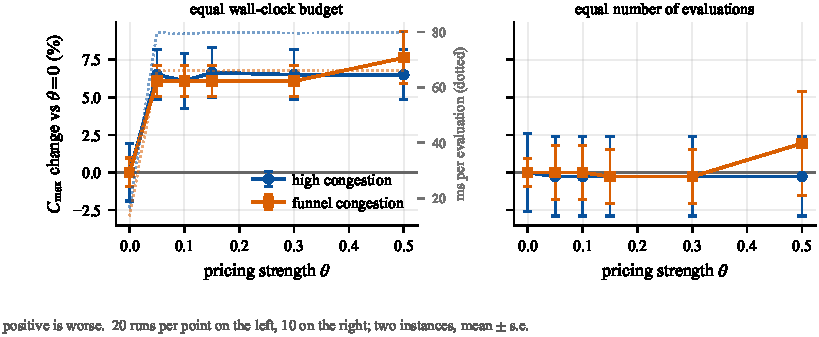
\includegraphics[width=\columnwidth]{fig/fig_theta.pdf}
\Description{Two panels of makespan change relative to theta equals zero against
pricing strength: under equal wall-clock the penalty is large and flat, under
equal evaluations it is absent.}
\caption{为层间接口定价。正值表示更差。在同挂钟预算下(左)惩罚在定价一开启时即出现,随后
在 $\theta$ 的十倍范围内保持平坦,并与右轴的单次评价成本同步。在同评价次数下(右)惩罚消失。
因此这种损害是"路由搜索变贵"的记账后果,而非价格误导了路由器的证据。}
\label{fig:theta}
%% 由 fig/fig_theta.py 从 clbs/experiments/theta_sweep.csv 与 theta_sweep_gen.csv 生成
%% (08-05 落盘,2 算例 x 10 种子,左图每点 20 次运行、右图 10 次)。
%% 更正:先前此处标注为"数据未落盘",实为误记——两个 CSV 均在盘上,已重新出图核对,
%% 图上形态与本小节正文一致(同挂钟下每个 theta 都变差且在十倍范围内平坦,同评价次数下归零)。
%% 该批次同属降本之前的测量,与第 5.5 小节引用的矩阵批次同期;定价机制在降本前后未改动,
%% 且其开销与剪枝无关(剪枝作用于派车试探,不作用于多标签路由),故该测量对它依然有效。
\end{figure}

实测的形态见图~\ref{fig:theta}:同挂钟下定价在我们试过的每个 $\theta$ 上都使完工时间变差且
显著,且惩罚在 $\theta$ 的十倍范围内保持平坦;同评价次数下同一比较与零无法区分。解释在评价
次数里——带价格的路由在同一预算内完成的评价次数只有不带价格时的约五分之一。\emph{定价并没有
把候选解排错序,它是把搜索饿死了。}

两项补充观察排除了其他读法。其一,$\theta$ 在本问题上不是一个有意义的旋钮:在跨两个数量级的
范围内,带价格的路由改变的是同样那几条路径、付出同样的总价格、返回同样的完工时间;累计价格
仅占总行驶时间的很小一部分,这个扰动太小,不足以推翻到达时刻在标量化目标
$\text{到达时刻}+\theta\cdot\text{价格}$ 中所施加的次序。只有当 $\theta$ 大到价格压过到达
时刻时,双重计价的损害才真正显现——而那时完工时间大幅恶化。其二,开销是\emph{结构性}的,而非
价格非零所致:同一次解码在带价格与不带价格下的耗时之比在每个 $\theta$ 上都相同,因为这笔钱
是为"每个节点维护一个 Pareto 前沿、每条弧尝试若干进入时刻"付的,与是否真的收取价格无关。
这正是引理~\ref{lem:label} 所预言的:引入第二判据即摧毁全序占优,单标签搜索必须让位给多标签
搜索。

我们把这个负结果写得较细,因为它比一个正结果更可迁移,也因为两种预算口径对它的\emph{幅度}
有分歧而对\emph{符号}没有。其中与实现无关的那部分论证是:无论价格来自对走廊容量的有限差分
探测还是来自关键链代理,它收取的都是一次\emph{后果已被全额支付}的占用费——那笔后果就在让行
车辆自己的到达时刻里。任何以完整无冲突解码作为适应度的架构都具有这一性质,而该性质的经验形态
就是"价格是惰性的"。于是决定比较结果的,变成了为一个惰性信号配备行动机器所需的代价。由此得到
的设计推论比我们原先想要的更锐利:\emph{在丰富一个层间接口之前,先检查接收层的目标函数是否
已经内部化了该接口要携带的东西;若已内部化,这种丰富不只是无益,而是严格有害的。}

%% 由独立小节降为上一节的子小节:它是消融的机制解释,不是本文的一级结论。
\subsubsection{机制层面的解释:代价与增益的稀释}
\label{sec:whycost}

上面的比较确立了凭证与错峰两个机制未能抵偿其代价,但没有解释\emph{为什么}。两项测量给出了
解释,而这两项解释同时也说明了预约表试探为何需要先降本才能显现价值。

\paragraph{算力去了哪里。}
把搜索的解码次数分开计数可以看到,冲突制导局部搜索消耗了全部解码次数中的很大一部分,而在它
所解码的邻居里,能真正改进完工时间的比例低于五十分之一。于是相当大的一份预算被花在一个"命中率
不足百分之二"的邻域上。要紧的比较不是那些改进是否真实——它们是真实的——而是同样这些解码次数
若还给种群循环会不会产出更多。在这样的命中率下确实会。

这个低命中率不是实现上的缺陷,我们为确认这一点花了一些功夫。该邻域按构造既小又有指向,每轮
至多 $L+2=7$ 个候选,且每一个都由下层指名;一个有指向的邻域仍然命中率低,意味着凭证所指认的
那些工序,改派或错峰之后并不能缩短关键链。我们尝试过三种针对性修补——按路径上的预期让行而非
按理想距离为改派候选打分、把错峰算子的相邻交换换成定向插入、以及接纳"完工时间不变但总让行
下降"的平台移动——每一种都在同评价次数下与未修改的算子独立比较,\emph{无一}达到显著。我们报告
这次尝试,因为它界定了结论的范围:失效在信号本身,而不在我们如何使用信号。

\paragraph{为什么信号弱:沿关键链的稀释。}
一份冲突凭证指明了某次让行事件的走廊、时段与对手任务,这恰是消除\emph{那一次}事件所需的信息。
但完工时间是经由一条链达成的,消除一处走廊延误通常会把另一个约束顶成紧约束——某道上游工序、
某台机械臂,或另一条走廊——因此实现的改进只是被消除延误的一个分数。我们自己的接受准则之所以
在每次接受移动后都重新提取关键链,正是出于这个原因。所以,当瓶颈只是众多量级相当的瓶颈之一时,
一个能指名瓶颈的反馈,其价值远低于它的量级所暗示的。

\paragraph{这如何解释预约表试探的两次不同结论。}
稀释同样作用于预约表感知的派遣:查表挑出的是当前这个任务送达最早的车,这是一个局部改进,其
对完工时间的影响也要经过同一条链被稀释。这正是它在降本之前难以显现的原因——一个被稀释后仍
为正、但幅度不大的收益,遇上 \CostMultBefore{} 倍的开销,净效果自然落进噪声里
(第~\ref{sec:whichcongestion}~小节引用的那批数据即是如此)。第~\ref{sec:speedup}~小节把开销
压到 \CostMultAfter{} 倍之后,同一个被稀释的收益就浮出了噪声。

由此得到本文在机制层面的核心判断,它比任何具体算子都更可迁移:\emph{在固定预算下,一个机制
能否成立,取决于"它被稀释后剩下的收益"与"它每次评价所增加的开销"之比,而这两者都是可以分别
测量、并可分别改进的。}凭证机制失效在分子——稀释后所剩太少,且三次针对性修补都无法把它抬起来;
派遣机制起初失效在分母,而分母是可以在不改变输出的前提下压低的。这个区分是我们选定后者、
放弃前者的全部理由。

\subsection{代价律与降本效果}
\label{sec:costlaw}

前面各小节反复用到"成本与评价次数是同一份资源的两种花法"这一论点。本小节把它本身作为对象来测,
因为本文承重机制的成立与否完全悬于此:同一个机制,在降本之前净效果落在噪声里,在降本之后显著
为正。

\paragraph{两种预算口径都不是中性的。}
图~\ref{fig:protocol} 给出各配置的单次评价成本与同预算内实际完成的评价次数。成本跨越两个数量
级,因此在同挂钟下便宜的配置能搜得多得多。这是为什么按相同代数比较是不可辩护的,也是为什么
对齐时间同样不是一个免费的选择。

\begin{figure}[t]
\centering
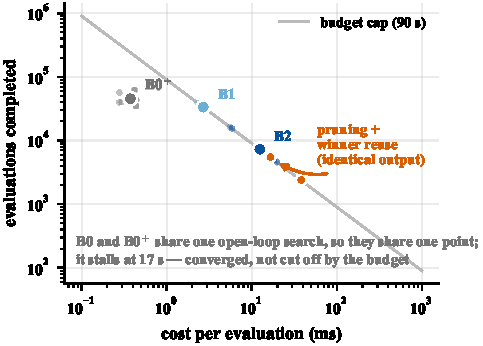
\includegraphics[width=\columnwidth]{fig/fig_protocol.pdf}
\Description{A log-log scatter of cost per evaluation against evaluations
completed, with the four ladder configurations lying along an equal wall-clock
hyperbola, and an arrow showing the pruning ablation moving one configuration
along that line without changing its output.}
\caption{固定挂钟预算把"单次评价成本"与"完成的评价次数"锁成一条双曲线(灰线,由实测预算
画出),各配置只能沿它移动。这就是本文反复引用的\emph{兑换率}:一个机制必须在每次评价里
买到的,多于它在评价次数上让出的。B0 与 B0$^+$ 共用同一次开环搜索,故共用一个点,差别只在
执行方式。橙色箭头是降本消融的两档——它是唯一一种\emph{不改变输出}就能沿该线移动的干预
(命题~\ref{prop:speedup_equiv}),因此这一段位移是纯粹的算力节省。}
\label{fig:protocol}
%% 由 fig/fig_protocol.py 生成(输出名 fig_protocol),数据源 clbs/output/ladder_cost.csv
%% 与 prune_ablation.csv;后者缺失时脚本自动省略橙色箭头而不报错。
\end{figure}

图~\ref{fig:protocols} 把同一组比较在两种口径下各做一遍。同代数口径不为"机制多做的那部分工作"
收费,因而系统性地偏袒复杂配置:在它之下预约表试探对规则派车有 \GainProbeSameGen{} 的显著
增益($p=\PProbeSameGen$),而同挂钟口径下同一比较在降本之前只剩 \GainProbeSameClock{}
($p=\PProbeSameClock$),几乎归零。两种口径都不错。同代数回答的是"该机制是否改进了一步搜索",同挂钟回答
的是"该机制是否改进了一次搜索";前者是机制设计问题,后者是是否值得部署的问题。不可辩护的是
报告其中一个却把它描述成另一个。

\begin{figure}[t]
\centering
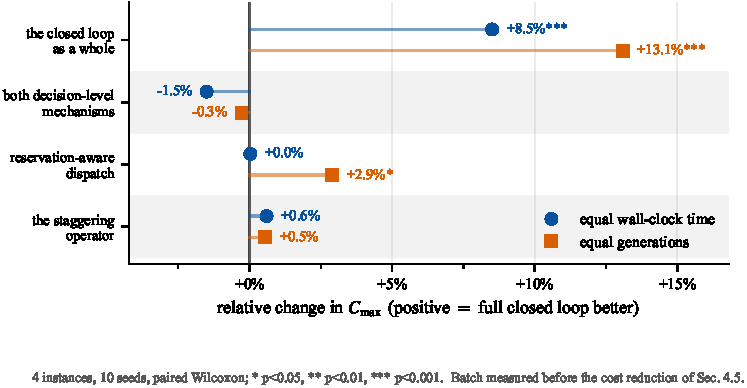
\includegraphics[width=\columnwidth]{fig/fig_protocols.pdf}
\Description{The same paired comparisons shown twice, once under an equal
wall-clock budget and once under an equal number of generations.}
\caption{同一组比较在两种预算口径下的读数。每一行按它所隔离的\emph{机制}命名,而非按被比较的
配置命名。两个标记之间的落差,就是表观增益中属于记账假象的那一部分:"预约表感知派遣"一行在
同代数下为 \GainProbeSameGen{}($p=\PProbeSameGen$),在同挂钟下降到 \GainProbeSameClock{}
($p=\PProbeSameClock$),即归零。该批次运行于第~\ref{sec:speedup}~小节的降本
\emph{之前},因此这一行同时是下文那个受控对照的动机。}
\label{fig:protocols}
%% 由 fig/fig_protocols.py 从 clbs/experiments/protocols.csv 生成(4 算例 x 10 种子)。
%% 行标签已从旧叙事的档位名(two-stage / open dispatch ...)改写为它所隔离的机制名,
%% 以免读者以为该图来自另一项研究;图脚已自报"降本之前"这一批次归属。
\end{figure}

\paragraph{代价律。}
派遣试探把每个运输任务的路由调用数从 $2$ 抬到至多 $2N_A$,故其开销随车队规模线性增长。剪枝
所依赖的下界在争用越弱时越紧,因而剪掉的候选越多;反过来,车队越大、争用越强,剪枝的效力越低。
第~\ref{sec:speedup}~小节的等价性自检已经显示出这个方向:六格中调用削减率最高的是最不拥堵的
一格(\RouteCallCutHi{}),最低的是车队最大的一格(\RouteCallCutLo{})——是效力衰减,不是失效。两个趋势合起来
\emph{预言}机制存在一个车队规模上的适用上界:在车队足够大且争用足够强时,试探的开销增长会
追上它的收益。必须强调这仍是一个预言:第~\ref{sec:whichcongestion}~小节在车臂比族的四个水平
上未能把它证实,那里的符号交替且四格无一显著。代价律本身(开销随 $N_A$ 线性、剪枝效力随 $N_A$
下降)是直接测得的,由它推出的上界则不是;把前者当作后者的证据,正是我们在前一版稿件里犯过
的错误。

\paragraph{降本值多少:一个只动降本的受控对照。}
把"降本"与"机制"分离开来度量是必要的,因为两者在时间上是先后引入的,若只并列两个批次的结果,
无法排除算例集与基线口径的差异。我们因此做了一个只动降本这一项的对照:同算例、同种子、同预算,
两档分别开启与关闭剪枝与胜者路径复用。

这个对照之所以干净,是因为命题~\ref{prop:speedup_equiv} 保证两项优化\emph{不改变输出}。我们
先把这条命题兑现为可观测的事实:在六个算例上各取六条随机染色体,两档给出的完工时间与派车序列
\emph{逐位相同},共 $36$ 组无一例外;而路由调用数合计减少 \RouteCallCut{}。既然输出相同,
关掉优化唯一的作用就是变慢,那么同挂钟预算下的完工时间差值就\emph{只}来自省下的算力,不掺
任何机制变化。

表~\ref{tab:prune} 给出结果:关$\to$开使完工时间再降 \GainPrune{}
(\WinPrune{} 胜 /\LosePrune{} 负,$p=\PPrune$),同预算内评价次数为 \EvalRatioPrune{} 倍,
单次评价加速 \SpeedupProbe{} 倍。它把两个批次之间那处表面矛盾接上了最后一环:同一个机制,
在降本前的矩阵批次上净效果落在噪声里(\GainProbePre{},$0/16$ 格显著),在降本后的阶梯批次上
显著为正,而中间这一步没有改变它做出的任何一个选择。

\begin{table}[t]
\caption{只改变剪枝与胜者路径复用的受控对照。两档输出逐位相同(已过等价性自检),故差值只来自
省下的算力。同算例、同种子、同挂钟预算;$n=60$ 配对。}
\label{tab:prune}
\small
%% 数字与 clbs/output/prune_ablation.csv / 运行日志一致;亦可用
%% py paper01/tab/gen_tables_ladder.py 从同一 CSV 重生成。
%% 由 prune_ablation.csv 汇总写入(与 tools/prune_ablation.py 日志一致),勿手工改数字
%% 6 算例 x 10 种子;开=exact(剪枝+复用),关=exact_noopt;输出逐位相同
\begin{tabular}{@{}lrrrrrr@{}}
\toprule
算例 & 争用强度 & 关 & 开 & $\Delta C_{\max}$ & 评价次数比 & 加速比 \\
\midrule
A funnel & 31.9\% & 44.80 & \textbf{42.10} & $-6.03\%$ & 2.21$\times$ & 2.23$\times$ \\
A high & 30.9\% & 41.60 & \textbf{37.70} & $-9.37\%$ & 2.40$\times$ & 2.41$\times$ \\
A low & 11.8\% & 60.50 & \textbf{57.00} & $-5.79\%$ & 2.79$\times$ & 2.81$\times$ \\
B NA/NM 0.5 & 15.8\% & 66.70 & \textbf{65.10} & $-2.40\%$ & 2.11$\times$ & 2.11$\times$ \\
B NA/NM 1.0 & 30.2\% & 51.90 & \textbf{48.90} & $-5.78\%$ & 2.31$\times$ & 2.31$\times$ \\
B NA/NM 2.0 & 32.4\% & 44.50 & \textbf{42.20} & $-5.17\%$ & 1.98$\times$ & 2.01$\times$ \\
\midrule
\emph{配对合计}(60 配对) & --- & --- & --- & $-5.60\%^{***}$ &
\multicolumn{2}{r}{50/0/10,\ $<10^{-4}$} \\
\bottomrule
\end{tabular}

\end{table}

\subsection{案例分析:甘特图与关键链归因}
\label{sec:casestudy}

汇总统计量说明机制平均起来有效,但不说明它在一次具体求解里\emph{做了什么}。本小节在单个漏斗
算例上把 B0 与 B2 的解并排画出,并沿关键链做归因,使前面的论证落到可以逐条核对的事件上。

图~\ref{fig:case_gantt} 是两个解的甘特图,机械臂与车辆画在同一时间轴上,车辆行的阴影段区分空载
与满载,让行等待单独着色。可以直接读出的三点是:开环解中让行等待成段地出现在站台附近的走廊上,
且集中在少数几辆车上;闭环解把这些等待大幅削去,代价是若干道工序被指派到了并非最快的机械臂;
以及闭环解的车辆利用更为均衡。第三点是前两点的结果而非另一个机制——它说明"用加工时间买邻近性"
这一权衡\eqref{eq:reassign} 在实际解中确实被行使了。

\begin{figure*}[t]
\centering
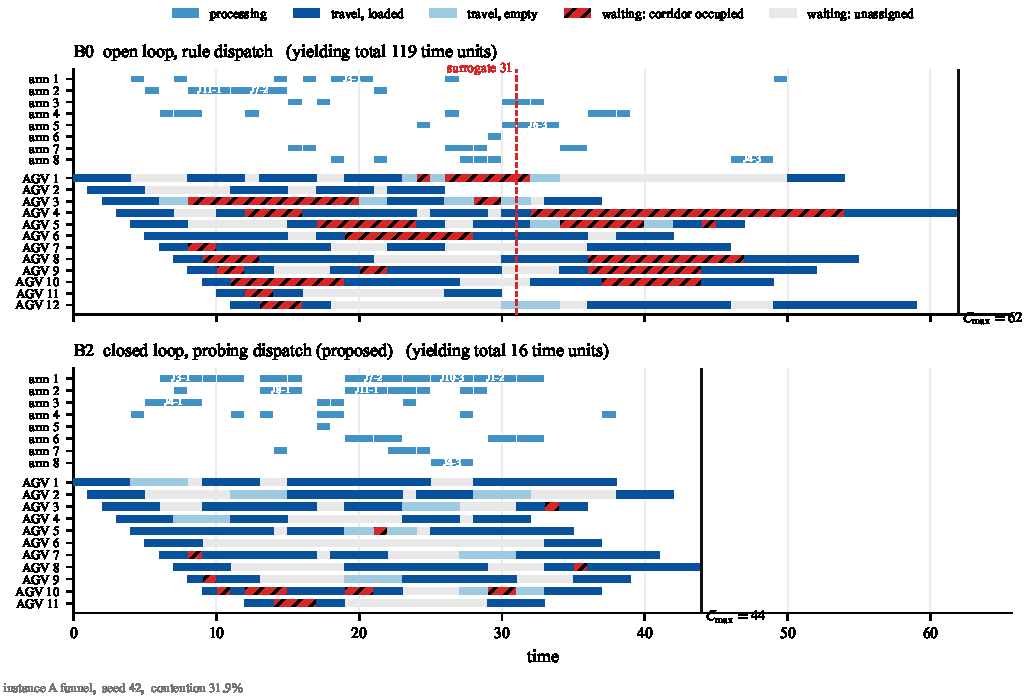
\includegraphics[width=\textwidth]{fig/fig_case_gantt.pdf}
\Description{Side-by-side Gantt charts of the open-loop and closed-loop
solutions on one funnel instance, with arms and vehicles on a shared time axis
and yielding waits shaded separately.}
\caption{同一漏斗算例上 B0(上)与 B2(下)的解。机械臂与车辆共用时间轴;车辆行区分空载段、
满载段,以及两类等待——按\emph{成因}分开着色是本图唯一要紧的设计:同一运输任务两段之间的
空隙是车被前方占用的走廊拦在停靠位上,即让行,也就是本文所处理的那种延误;不同任务之间的
空隙则是车无活可干,属于车队规模的症状。两者若同色,读者就会把其中一种归因成另一种。
图内文字为英文以便与代码输出一致。}
\label{fig:case_gantt}
%% 由 fig/fig_case_gantt.py 从 clbs/output/case_study/*.json 生成(tools/ladder_diag.py
%% 的 --case-study 落盘)。让行/空闲的区分由脚本从相邻段的 task 字段推出,不是另存的标注。
\end{figure*}

图~\ref{fig:case_chain} 沿关键链做归因,把每一环按表~\ref{tab:attrib} 的五类标注着色。它使
第~\ref{sec:whycost}~小节的稀释论证可视:在 B0 的链上走廊环占据显著比例,而在 B2 的链上它们大
体被消除,顶上来的是机械臂环与上游工序环。这正是"消除一处走廊延误会把另一个约束顶成紧约束"
的直接图示,也解释了为何指名瓶颈的反馈其价值低于它的量级。

\begin{figure}[t]
\centering
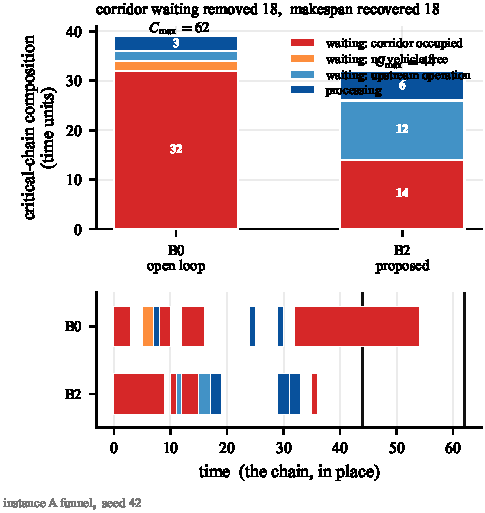
\includegraphics[width=\columnwidth]{fig/fig_case_chain.pdf}
\Description{The critical chain of the open-loop and closed-loop solutions,
with each link coloured by its attribution label.}
\caption{关键链归因。上:两档关键链的构成,每一环按表~\ref{tab:attrib} 的标注着色;标题直接
并列"被消除的走廊等待"与"实际收回的完工时间",二者之差即被顶上来的约束吸收掉的部分。
下:同一条链在时间轴上的原位,以表明上方的柱是一条链的分解,而非若干互不相关事件的直方图。
闭环解中走廊环大体消失,顶上来的是机械臂与上游工序——这就是稀释效应的直接图示。}
\label{fig:case_chain}
%% 由 fig/fig_case_chain.py 从同一批 case_study/*.json 生成;归因标签直接取
%% algorithm/decoder.py 的 critical_chain(),五类标签一个不并、不归入 other。
\end{figure}

%% 原此处的"有效性威胁"独立小节已整体并入第 6 章的局限小节(6.3)。独立成节是实证软件
%% 工程的惯例,在运筹与调度类刊物中少见,留在实验章会削弱结果章的正面叙事。

\subsection{外部标定:公开基准上的退化对标}
\label{sec:external}

前面所有比较都是\emph{内部}比较:同一套代码的不同配置在同一批自建算例上相比。这排除了配置
之间的实现方差,却留下一个它无法回答的问题——这套实现本身的绝对水平如何。若上层搜索本身很弱,
配置之间的差值仍然可信,但"绝对完工时间"这一列就只反映实现质量。本小节用一个外部参照来标定它。

\paragraph{比较的对象是什么,不是什么。}
删去排他约束~\eqref{eq:excl} 之后,本文模型精确退化为标准的 FJSP\_PT
(第~\ref{sec:Chapter_III}~节),即与公开基准\emph{同一个数学问题};此外取
$\delta_{\mathrm{ret}}=0$ 以对上这批算例的完工时间定义,而它本就是本文模型的一个参数
(表~\ref{tab:notation}),不是又一次删约束。因此这个比较是合法的,
但它检验的是\emph{上层搜索},而不是本文的框架:退化之后既没有走廊争用,也就没有任何反馈可言,
本文的两条机制在此全部失效。我们做它的唯一目的是标定绝对水平,并把结果与内部比较\emph{分表
报告}——若把两者并进一张表,读者将无法判断哪一条结论靠哪一批数据。

\paragraph{算例与口径。}
取 Homayouni 与 Fontes~\cite{homayouni2021production} 整理的 \PubNInst{} 个算例
(源自 Fattahi 等~\cite{fattahi2007mathematical}的 FJSP 算例,$2$--$12$ 个工件、$4$--$48$ 道
工序、$2$--$8$ 台机器),按文献口径取两辆车~\cite{lim2023twophase}、成品不回运,行驶时间
\emph{原样}取所发布的矩阵而不做任何最短路合成——第~\ref{sec:instances}~小节已说明其中
\PubNLayoutBad{} 个矩阵不是任何图的最短路闭包,做合成会改变算例。这在退化档里是相容的:
排他约束一旦删去,路网 $G$ 就只通过 $t^{*}$ 进入模型,而 $t^{*}$ 是它唯一被用到的量;因此直接
把所发布的矩阵当作 $t^{*}$ 即可,并不需要存在一张与之一致的 $G$。反过来说,这也正是这批算例
\emph{只能}用于退化档的原因——争用需要的是 $G$ 本身,而它不存在。口径的正确性不是靠声明,
而是靠两个算例的逐位手算核对:$\mathrm{SFJST}01$ 的
文献最优值 $70$ 恰等于"站台到机器的行程 $4$ 加两道工序 $45+21$",$\mathrm{SFJST}03$ 的 $223$
恰等于某台机器上三道工序的紧密排列,两者都\emph{不含}回运行程;若把回运计入,前者应为 $78$。
参照值取自文献:\PubNOpt{} 个算例有 MILP 证明的最优值~\cite{homayouni2021production},其余
$4$ 个取已发表最好值~\cite{lim2023twophase}。

\paragraph{结果。}
表~\ref{tab:external} 给出 \PubNInst{} 个算例 $\times$ \NSeeds{} 个种子的结果。三条硬性判定
在全部 $200$ 次运行中通过:没有低于复合下界的解,没有校验失败,且在有可证最优值的那
\PubNOpt{} 个算例($160$ 次运行)上没有任何一次低于该值。最后一条是这里最要紧的——退化档与
文献是同一个问题,可证最优值是硬地板,若我们"赢"了它,那不是结果好,而是转换或口径有错。
$\PubNMatch{}/\PubNInst{}$ 个算例上最优解与参照值\emph{逐位相同},其中 $10$ 个小型算例
(\textsc{sfjst}01--10)全部命中;\PubNInst{} 个算例的平均间隙为 \PubGapMean{}
(中位 \PubGapMed{})。间隙随规模上升,但\emph{并非逐个算例单调}——\textsc{mfjst}03 与
\textsc{mfjst}06 都比各自更小的邻居更好;真正稳定的是尾部:四个最大算例($32$--$48$ 道工序)
的均值为 \PubGapBig{},最差 \PubGapMax{},而不超过 $24$ 道工序的那 $16$ 个算例无一超过
$5.45\%$。

\begin{table}[t]
\caption{公开基准上的退化对标(排他约束删去,与文献同一问题)。"参照"列的
\textsc{opt} 为 MILP 证明的最优值、\textsc{bk} 为已发表最好值;间隙以 \NSeeds{} 个种子的最优
解计。星号标出最优解与参照值逐位相同者。数据:\texttt{experiments\_database/gap\_ideal.csv}。}
\label{tab:external}
\centering
\small
\begin{tabular}{lrrrrrr}
\toprule
算例 & 工序 & 参照 & \multicolumn{1}{c}{值} & 最优 & 均值 & 间隙 \\
\midrule
SFJST01 & 4 & \textsc{opt} & 70 & 70\rlap{$^*$} & 70.0 & 0.00\% \\
SFJST02 & 4 & \textsc{opt} & 111 & 111\rlap{$^*$} & 111.0 & 0.00\% \\
SFJST03 & 6 & \textsc{opt} & 223 & 223\rlap{$^*$} & 223.0 & 0.00\% \\
SFJST04 & 6 & \textsc{opt} & 359 & 359\rlap{$^*$} & 359.0 & 0.00\% \\
SFJST05 & 6 & \textsc{opt} & 123 & 123\rlap{$^*$} & 123.0 & 0.00\% \\
SFJST06 & 9 & \textsc{opt} & 324 & 324\rlap{$^*$} & 324.0 & 0.00\% \\
SFJST07 & 9 & \textsc{opt} & 409 & 409\rlap{$^*$} & 409.0 & 0.00\% \\
SFJST08 & 9 & \textsc{opt} & 269 & 269\rlap{$^*$} & 269.5 & 0.00\% \\
SFJST09 & 9 & \textsc{opt} & 220 & 220\rlap{$^*$} & 222.0 & 0.00\% \\
SFJST10 & 12 & \textsc{opt} & 531 & 531\rlap{$^*$} & 531.0 & 0.00\% \\
MFJST01 & 15 & \textsc{opt} & 485 & 485\rlap{$^*$} & 485.0 & 0.00\% \\
MFJST02 & 15 & \textsc{opt} & 463 & 476 & 483.4 & 2.81\% \\
MFJST03 & 18 & \textsc{opt} & 482 & 482\rlap{$^*$} & 504.7 & 0.00\% \\
MFJST04 & 21 & \textsc{opt} & 576 & 586 & 623.0 & 1.74\% \\
MFJST05 & 21 & \textsc{opt} & 532 & 561 & 592.8 & 5.45\% \\
MFJST06 & 24 & \textsc{opt} & 652 & 677 & 728.3 & 3.83\% \\
MFJST07 & 32 & \textsc{bk} & 898 & 965 & 1023.3 & 7.46\% \\
MFJST08 & 36 & \textsc{bk} & 900 & 970 & 1027.0 & 7.78\% \\
MFJST09 & 44 & \textsc{bk} & 1098 & 1226 & 1279.2 & 11.66\% \\
MFJST10 & 48 & \textsc{bk} & 1230 & 1389 & 1473.0 & 12.93\% \\
\bottomrule
\end{tabular}
\end{table}

\paragraph{这个间隙是能力上界,不是预算不足。}
一个显然的反驳是我们给的算力太少:在文献报告的 \PubNOpt{} 个可证最优值里,最大那个算例的
MILP 求解耗时将近十小时(\textsc{mfjst}06,$34\,796$ 秒),而我们每次运行只用数秒。我们因此把
预算提高一档(代数上限提至五倍、早停阈值提至 $3.3$ 倍,实测挂钟增至 \PubBudgetRatio{} 倍),
在 $10$ 个 \textsc{mfjst} 算例上重跑——即表~\ref{tab:external} 的后十行,间隙全部集中在这里。
这十个算例的平均间隙从 \PubGapLoBudget{} 降到 \PubGapHiBudget{}(此处的基数只含这十个,故与
上文 \PubNInst{} 个算例的 \PubGapMean{} 不同口径),即 \PubBudgetRatio{} 倍算力只买到
$\PubBudgetGainPP$ 个百分点;十个中有 \PubBudgetNoGain{} 个\emph{一点没降},最大的那个算例从
$12.93\%$ 只降到 $12.85\%$。更能说明问题的是停机原因:两档预算下的全部 $300$ 次运行\emph{无一}
撞到代数上限,都是早停阈值触发的自然收敛,故加大预算买到的并不是"跑得更久"。因此这个间隙主要
是上层搜索的能力边界,而非预算标定问题——我们如实报告它,并把"在大规模算例上缩小这个间隙"
列入第~\ref{sec:future_work}~小节。

\paragraph{一个副产品:复合下界的松弛量得以分离。}
本文的复合下界与\emph{所求得的最好解}之间的间隙中位数为 \LBGapMed{},而在自建算例上无法判断
这个数里有多少是\emph{下界松}、多少是\emph{搜索差}——两者都会把它撑大,而最优值未知,无从
拆开。公开算例给出了这个分解。口径只取那 \PubNOpt{} 个有可证最优值的算例:另外 $4$ 个的参照
是已发表最好值,而真实最优只可能更小,拿它当分母会把"下界松"这一份高估,故这里取严的那一档。
在这 \PubNOpt{} 个算例上,同一个复合下界距\emph{可证最优值}的中位数为 \PubLBSlack{},而距本文
所得最好解的中位数为 \PubLBTotal{};逐算例作差,"搜索欠缺"这一份的中位数是
$\PubLBResidMed$ 个百分点(因为其中多数算例本就命中了最优),最大也只有 $\PubLBResidMax$ 个
百分点。也就是说,这批算例上的间隙几乎全部来自下界自身的松弛。这个结论不能直接搬到自建算例
上——那里有争用,而该下界完全忽略争用,故在那里只会\emph{更}松;但它把证据的天平明确推向
"下界松"这一侧,而这正是第~\ref{sec:limitations}~小节的局限 (4) 所说、在自建算例上无从区分的
那件事。

\section{结论}
\label{sec:Chapter_VI}

本文研究异构机械臂加工与 AGV 无冲突路由的一体化调度,其前提是文献通常回避的那一条:行驶时间
\emph{由路由决策产生},而不是从一张矩阵里读出来。在这一设定下,我们没有停留在"耦合两层是否
有益"这个已有答案的问题上,而是问了一个更具体的:当预算固定、任何信息都要用放弃掉的评价次数
来支付时,\emph{哪一种}层间信息值得它的代价,以及如何让它付得起。

\subsection{结论与贡献}
\label{sec:contributions}

\textbf{(1) 一个双反馈通路的闭环双层框架。} 上层以 memetic 算法搜索指派与排序,下层以时间窗
预约做无冲突路由;每一代每一个个体的适应度都是下层完成全部运输任务规划之后的完工时间,因此
上层从不优化代理目标。命题~\ref{prop:decodable} 与引理~\ref{lem:label} 保证任何染色体都可
解码、评价相对第~\ref{sec:Chapter_III}~节的冲突模型是精确的,且不需要任何修复算子。把拥堵搬进
搜索目标这一步,在规则派车下值 $\GainLoopRule$($p=\PLoopRule$),在试探派车下值
$\GainLoopProbe$($p=\PLoopProbe$)。

\textbf{(2) 预约表感知的车辆派遣,以及使它付得起的降本。} 选车是整个框架中最后一处可以用估计
代替事实的环节,我们把它闭合:选车前对预约表做两段式试探,用实际可达的送达时刻代替理想最短路
的估计。在闭环内部它值 $\GainProbeLoop$($p=\PProbeLoop$)。这个机制的关键困难不在于设计而
在于代价——它使单次评价贵 \CostMultBefore{} 倍,足以在同挂钟预算下把自身收益吃光。我们给出
两项优化(可采纳下界剪枝与胜者路径复用),并\emph{证明}它们不改变输出
(命题~\ref{prop:speedup_equiv}),又以逐位等价性自检加以实证;它们把路由调用减少
\RouteCallCut{},把成本倍数压到 \CostMultAfter{}。因此本文对这一机制的主张是完整的:它有效,
而且我们说明了它为何一度看不出有效,以及如何让它有效。

\textbf{(3) 主效应与次效应的分工,以及支撑该结论的实验协议。} 闭环是主效应,并且是逐格
稳健的:$\NCases$ 个算例格中 $\CellsSigLoop$ 格自身即达显著。预约表感知派遣在开环与闭环下
的合计口径上都显著($\GainProbeOpen$,$p=\PProbeOpen$;$\GainProbeLoop$,$p=\PProbeLoop$),
但逐格只有 $\CellsSigProbe$ 格显著,因此它是一个"平均起来成立"的效应,本文不就它在何种结构
上兑现作主张。端到端 $\GainEndToEnd$ 接近独立乘积 $\GainIndepProduct$(近加性,无正交互);
开环试探单独远不能代替闭环。这对"先排产、后解冲突"给出结构性判断:第二阶段能显著挽回一部分,
但主效应仍留在桌面上。支撑它的是 $2\times2$ 析因与统一执行器口径:无论计划从哪来,都必须经
同一个无冲突路由器执行、过同一个校验器,报的都是可实现的完工时间。

\subsection{主要洞见}
\label{sec:insights}

有三条判断的适用范围比本文的具体算子更宽,我们认为它们是本文更值得带走的部分。

\textbf{接口丰富之前,先查接收层是否已经内部化了它要携带的东西。} 我们完整实现了走廊时段定价,
它在同挂钟预算下系统性地有害。原因不是估计器不好,而是架构性的:由争用造成的延误已经完整体现
在让行车辆自己的到达时刻里,并经 \eqref{eq:bind} 传播进完工时间被适应度计入;再对同一次占用
收一次价格等于把它数了两遍。任何以完整无冲突解码作为适应度的框架都具有这一性质,其经验形态
就是"价格是惰性的"。而一旦引入价格作为第二判据,引理~\ref{lem:label} 的全序占优即被摧毁,
单标签搜索必须让位给多标签搜索——这笔钱无论是否真的收取价格都要付。

\textbf{区分"改进一个决策"与"改进一次测量"。} 指名瓶颈的反馈买到的是局部改进,而完工时间是
经由一条链达成的,消除一处延误通常把另一个约束顶成紧约束,因此实现的改进只是被消除延误的一个
分数。修正目标函数则不同:它不作用于链上任何一环,而是改善搜索将要比较的\emph{每一个}候选解的
排序,因此无须经受稀释。这个不对称解释了为什么冲突凭证制导的局部搜索在三次针对性修补之后仍
不划算,而它也同时解释了预约表试探为何需要先降本——被稀释后仍为正但幅度不大的收益,遇上足够
大的开销就会落进噪声。

\textbf{在固定预算下,机制的成立与否是一个可分解、可分别改进的比值。} 分子是"稀释后所剩的
收益",分母是"每次评价所增加的开销"。凭证机制失效在分子,而分子难以人为抬高;派遣机制起初
失效在分母,而分母可以在不改变任何输出的前提下压低。这个区分不仅是本文的取舍依据,也给出了
一条可操作的诊断顺序:先测一个机制的开销倍数与其被稀释后的收益,再决定是改进它还是放弃它。
它同时意味着一件容易被忽略的事——\emph{工程上的降本可以是方法学上的贡献},因为在同预算口径下
降本与增效是同一件事。

\subsection{局限}
\label{sec:limitations}

\textbf{(1) 算例族。} 全部算例格共用一个规模与一套布局模板。我们变化的是分析判定为关键的那些
因子(布局、车臂比、柔性),但规模与拓扑类型是固定的,我们不就机制如何随规模变化作任何主张。
异质度 $H$ 不在这一族的扫描之内——它固定在 $0.3$,其四个水平的扫描来自
第~\ref{sec:whichcongestion}~小节那批规模更小的独立算例,故"收益不随 $H$ 上升"这一条是在
\emph{那个}规模上得到的,我们不把它外推到本族。
用以刻画布局族的争用强度也是一个粗糙的一维摘要:它给出"让行占行驶时间的比例",却不区分其中
有多少是指派可以绕开的,这正是布局族上收益与争用强度并不严格同序的一个可能原因。

\textbf{(2) 逐格统计功效。} 每格 $\NSeeds$ 个种子足以分辨闭环效应($\CellsSigLoop/\NCases$
格自身显著),却不足以分辨预约表感知派遣($\CellsSigProbe/\NCases$ 格)。后者的量级只有数个
百分点,与本问题的种子间离散度同量级,因此我们只能在 $\NPairs$ 个配对的合计口径上确认它为正,
无法定位它在哪些结构上兑现。这不是一个可以靠改写论述绕开的限制,而是需要把种子数提高约一个
数量级才能解除的限制;第~\ref{sec:costlaw}~小节的代价律所预言的车队规模上界,因此在本文中
仍是未被检验的预言。我们把这一条单列,是因为在同类文献中,逐格符号被当作适用区间来叙述是
常见做法,而按本文的功效水平那样做会是在读噪声。

\textbf{(3) 公开基准只能标定上层,不能检验框架。} 通行的 FJSP\_PT 基准把行驶时间发布为一张
常数矩阵;第~\ref{sec:instances}~小节已就实际取用的那一族查明,\PubNLayoutAsym{}/\PubNLayout{}
张矩阵不对称因而不可能是任何无向走廊网络的 $t^{*}$,其中 \PubNLayoutBad{} 张连最短路闭包都
不是。既然不存在与之一致的通道网络,争用在\emph{这类矩阵算例}上就无从定义,在其上运行本文方法
必须先删掉本文所讨论的那条约束。
第~\ref{sec:external}~小节做了这个退化比较并如实报告:它检验的是上层搜索而非本框架,因为退化
之后争用不存在,本文的两条机制全部失效。结论有两面。好的一面是绝对水平得到了外部标定:
$\PubNMatch{}/\PubNInst{}$ 个算例上取得与文献逐位相同的完工时间,$10$ 个小型算例全部命中可证
最优,且没有任何一次运行低于可证最优值。不好的一面是间隙随规模恶化,四个最大算例平均
\PubGapBig{};把算力提到 \PubBudgetRatio{} 倍只换来 $\PubBudgetGainPP$ 个百分点,故这是能力
边界而非预算问题。需要说清楚这一点对前文各结论的影响。它\emph{不}威胁主效应,首要的理由不是
量级而是口径:上层搜索的绝对强弱是各档\emph{共有}的,因此它本身无法制造出各档之间的差值,而
本文主张的正是差值。这不等于说差值与搜索强度无关——那是一个我们没有检验的问题,已列入
第~\ref{sec:future_work}~小节。量级只是一重旁证,且我们不夸大它——闭环增益 \GainLoopRule{}
约为最大算例那档间隙
\PubGapBig{} 的两倍、为 \PubNInst{} 个算例平均间隙 \PubGapMean{} 的七倍左右,并非高出一个
量级。但它确实意味着,几个百分点量级的次效应(如 \GainProbeLoop{})所处的尺度与上层搜索自身
离最优的距离\emph{相当},这与局限 (2) 指出的"次效应与种子间离散度同量级"是同一件事的两个
侧面:次效应之所以脆弱,既因为噪声与它同量级,也因为它落在实现本身离最优的距离之内。
带无冲突运输约束的这一支目前仍没有标准基准:文献~\cite{vanos2026exact} 明确指出这一点,
并转而采用此前仅有的两份自建算例。其模型、工具、算例与全部解均已公开,但它与本文在\emph{冲突
语义}上并不同构。差别不在路网的方向性上:该文虽把路网声明为单向图,其算例却把每条无向边展开为
方向相反的两条弧,故通行实际仍是双向的。差别在\emph{预约单位}——该文把冲突定义为两车同时占据
同一节点或在同一时刻交换节点,且只有装卸站允许多车同时在场,即预约的是\emph{节点};本文的走廊
是双向排他资源,两个方向共用同一份占用,节点是容量充裕的零测度通过点,即预约的是\emph{边}。
此外该文要求同一机械臂连续加工同一工件的两道工序时须有车辆在场
支持装卸,而本文假定卸料瞬时完成、机械臂的释放不受 AGV 牵制。因此在其算例上运行本文方法所比较
的将是两次模型翻译,而不是两个方法,我们没有做。
还有一份公开算例不能用上一段的理由排除,需单独交代。Lyu 等~\cite{lyu2019approach} 的算例族
同时具备可选机、随机器而变的加工时间与显式路网,且其路网是\emph{双向}的,并明确规定"同一时刻
一条路段只能通行一辆车",即它预约的也是\emph{边}——在冲突语义这一维上它与本文同构,而不像
\cite{vanos2026exact} 那样需要翻译;它还给出了按车队规模分档的完工时间参照值。把它排除的是另外
两条理由。其一,它在边排他之外\emph{还}要求任一节点在任一时刻只容一辆车,而本文的节点是零测度的
通过点;因此本文模型是它的\emph{松弛},在其算例上运行本文方法可能给出在其模型下并不可行的解,
完工时间反而低于其发表值——那不是更优,而是口径不同、数字不可比。其二,其规模较大的那一组只
给出路网拓扑与机器位置,未发表逐段行驶时间(全文仅声明车辆匀速),故在其上比较时边权将是我们
引入的假设而非该文的数据。这一条看上去有个自然的补法,实际没有:那几张布局图都画成规整网格、
不标边权,似可一律取单位边权;但该文\emph{唯一}给出逐段时长的那个算例,其布局图的画法与它们
完全相同,而相邻段的时长却取了三种不同的值——可见图是示意而非按比例,"每段看上去一样长"在该文
中并不蕴含"每段耗时相同"。于是这一族的边权是真未知,任何补法都与该文自身仅有的那处数据相抵触,
而其按车队规模分档的参照值一旦换了边权便不再可比。这一份的正面意义在于,本文
"双向走廊 + 边排他"的建模选择在文献中已有先例,并非为本文方便而设。

\textbf{(4) 下界质量与最优距离。} 复合下界是松的,与所求得的最好解之间的间隙中位数为
\LBGapMed{}。它的作用是数量级核查与回归防护,不是最优性证书。在自建算例上这么大的间隙无法
区分"搜索失败"与"下界松弛",因为两者都会把它撑大而最优值未知。第~\ref{sec:external}~小节的
退化对标给出了一次分解:在有可证最优值的那 \PubNOpt{} 个公开算例上,同一个下界距可证最优的
中位数为 \PubLBSlack{},而距本文最好解的中位数为 \PubLBTotal{},逐算例作差后"搜索欠缺"这一份
最大只有 $\PubLBResidMax$ 个百分点——即间隙几乎全部来自下界自身的松弛。这个分解不能直接搬回
自建算例:那里存在争用,而该下界完全忽略争用,故在那里只会\emph{更}松,搬过去只会高估"下界松"
这一份。我们因此仍不就自建算例上解与最优解的接近程度作定量主张,但这一次的原因已经收窄为
缺少那些算例的最优值,而不再是两种成因无从判断。

\textbf{(5) 单一实现。} 所有配置共用一套代码,这消除了配置之间的实现方差,但也意味着绝对完工
时间反映的是该实现的质量。各配置之间的差值是内部比较,不受此影响;与已发表方法的对比会受影响。
第~\ref{sec:external}~小节部分地缓解了这一条:在公开算例上,该实现在 $10$ 个小型算例上全部
达到可证最优、在 \PubNInst{} 个算例上平均落后 \PubGapMean{},故它不是一个弱实现。但缓解是
部分的——那批算例没有争用,因而未标定下层路由与预约表这一半代码的绝对水平,而它恰是本文
新增的那一半。

\textbf{(6) 负面结果的作用域。} 两个负对照机制都是在一个由纯 Python 实现标定的预算下被判定的。我们
的比较所测量的是"成本与评价次数之间的兑换率",且它是在共享同一实现的配置之间测得的,故对一个
\emph{常数倍}的加速是稳健的;但它对各部件\emph{相对}成本的改变并不稳健。这正是本文降本一节的
意义所在——我们已经在派遣上演示了改变相对成本可以翻转结论。因此我们的结论应被理解为:这些机制
在\emph{当前代价下}不划算,而非它们不可能划算。

\textbf{(7) 收敛性。} 交换乘子或价格的双层方案有时可被证明收敛到不动点,本框架不能,我们也
不作此主张。下层是优先级式而非联合最优,上层是非凸组合空间上的随机搜索,层间传递的是证据而非
可充当 Lyapunov 函数的量。

\subsection{未来工作}
\label{sec:future_work}

\textbf{增量式评价。} 解码器的状态严格向前流动,因此只在序列某位置之后被扰动的邻居,其之前的
全部事件与预约都不变。一个能够只重解被扰动部分的增量式评价器,会恰好降低本文中失效的那些机制
的代价,冲突制导邻域是在它之下最值得重测的第一个候选。按上一小节的比值框架,这是从分母一侧
再做一次尝试。

\textbf{链可替代性作为算例维度。} 稀释论证预言:关键链越不可替代——即车间只有一个主导瓶颈而
非许多量级相当的瓶颈——制导型反馈就越有价值。本文的布局族变化的是争用的\emph{可避免性}而非
链的\emph{可替代性},且我们为量化前者引入的漏斗占比 $\varphi$ 未能区分它本要区分的两个族
(第~\ref{sec:features}~小节)。一个按链可替代性参数化的算例族,配上一个经过"它声称度量的那个
操纵"检验过的指标,才能真正检验这条解释,而不只是与之不矛盾。这里的方法要求值得单独说明:一个
结构指标在被用来解释结果之前,应当先在一组\emph{已知答案}的算例上验明它确实随该结构变化——
$\varphi$ 和本文的争用强度都没有经过这道手续,而布局族上收益与争用强度并不严格同序,很可能
正是这道手续缺失的代价。

\textbf{大规模算例上的上层搜索。} 第~\ref{sec:external}~小节把上层搜索的绝对水平测了出来:
小规模上达到可证最优,而在 $32$--$48$ 道工序的算例上落后 \PubGapBig{},且这个间隙对算力
不敏感——提到 \PubBudgetRatio{} 倍只降 $\PubBudgetGainPP$ 个百分点。因此它需要的不是更长的
运行,而是编码或邻域上的改动;线索是那四个算例的种子间标准差达其均值的 \PubCvBig{},而每次
运行都是自然收敛(触发早停)而非被预算掐停,这指向"陷在不同的局部结构里"而非"尚未收敛"。
这项工作与本文的机制结论\emph{正交}:上层变强会同时
抬高阶梯上的每一级,而各级之差才是本文的主张;但它会改变次效应能否从噪声中被分辨出来,因此
它也是把局限 (2) 解除掉的一条路。

\textbf{小规模精确解。} 已有工作表明基于逻辑的 Benders 分解可以为该问题类给出精确
解~\cite{vanos2026exact},且其实现与算例均已公开。小规模精确解可以确定间隙中有多少是可回收的
——这正是本文因下界过松(局限 (4))而无法回答的问题——也可以检验那些在启发式搜索下不划算的机制,
在搜索更强时是否依然不划算。可行的做法不是把本文方法搬到对方算例上(冲突语义不同构,见局限 (3)),
而是把该精确方法的冲突模型改写为走廊排他的版本后,在本文的小规模算例上求解;改写的正确性本身
需要单独验证,故这是一项独立的工作而非一次补充实验。

\textbf{把次效应的适用区间测出来。} 本文能确认预约表感知派遣平均为正,却无法说出它在哪些结构
上兑现:逐格 \NSeeds{} 个种子只够分辨闭环那一级的效应(局限 (2))。代价律给出了一个明确且
可证伪的预言——存在一个车队规模,超过它之后试探的开销增长追上它的收益——而检验这个预言需要的
不是新机制,只是把种子数提高约一个数量级,并在车臂比上取更密的水平。这类"只花算力不花想法"
的后续工作在文献中常被略过,但对一个其效应量级只有数个百分点的机制而言,它恰恰是把"平均有效"
变成"知道何时有效"的唯一途径。

\textbf{动态运行。} 本文的建模假定加工时间已知、工件集固定。在线到达与车辆故障会改变本文所报的
这套算术,因为那时一个机制的价值还包括它修复排程的速度,而不只是它构建排程的质量;一个必须
从头重解的廉价评价器,与一个能把损害局部化的制导机制相比,结论可能不同。


%\section*{Acknowledgments}
%This work was supported partly by Key Laboratory of Computer Network and Information Integration (Southeast University) of Ministry of Education of China under Grants NO. 93K-9 and Jiangsu Provincial Key Laboratory of Network and Information Security under Grants No.BM2003201.

%%
%% The next two lines define the bibliography style to be used, and
%% the bibliography file.
\bibliographystyle{ACM-Reference-Format}
\bibliography{reference-base}


%% 本文没有附录。acmart 的 \appendix 若不带任何内容会在目录与页眉里留下一个空标题,
%% 故直接不声明;若日后要加附录,在此处恢复 \appendix 再写 \section。

\end{document}
\endinput
%%

